%%%%%%%%%%%%%%%%%%%%%%%%%%%%%%%%%%%%%%%%%%%%%%%%%%%%%%%%%%%%%%%%%%%%%%%%%%%%%%%
%                       CARREGA DE LA CLASSE DE DOCUMENT                      %
%                                                                             %
% Les opcions admissibles son:                                                %
%      12pt / 11pt            (cos dels tipus de lletra; no feu servir 10pt)  %
%                                                                             %
% catalan/spanish/english     (llengua principal del treball)                 %
%                                                                             % 
% french/italian/german...    (si necessiteu fer servir alguna altra llengua) %
%                                                                             %
% listoffigures               (El document inclou un Index de figures)        %
% listoftables                (El document inclou un Index de taules)         %
% listofquadres               (El document inclou un Index de quadres)        %
% listofalgorithms            (El document inclou un Index d'algorismes)      %
%                                                                             %
%%%%%%%%%%%%%%%%%%%%%%%%%%%%%%%%%%%%%%%%%%%%%%%%%%%%%%%%%%%%%%%%%%%%%%%%%%%%%%%
 
\documentclass[11pt,spanish,listoffigures,listoftables]{tfgetsinf}

%%%%%%%%%%%%%%%%%%%%%%%%%%%%%%%%%%%%%%%%%%%%%%%%%%%%%%%%%%%%%%%%%%%%%%%%%%%%%%%
%                     CODIFICACIO DEL FITXER FONT                             %
%                                                                             %
%    windows fa servir normalment 'ansinew'                                   %
%    amb linux es possible que siga 'latin1' o 'latin9'                       %
%    Pero el mes recomanable es fer servir utf8 (unicode 8)                   %
%                                          (si el vostre editor ho permet)    % 
%%%%%%%%%%%%%%%%%%%%%%%%%%%%%%%%%%%%%%%%%%%%%%%%%%%%%%%%%%%%%%%%%%%%%%%%%%%%%%%

\usepackage[utf8]{inputenc} 

%%%%%%%%%%%%%%%%%%%%%%%%%%%%%%%%%%%%%%%%%%%%%%%%%%%%%%%%%%%%%%%%%%%%%
% Para conseguir que la tabla de contenido no salga en rojo
%%%%%%%%%%%%%%%%%%%%%%%%%%%%%%%%%%%%%%%%%%%%%%%%%%%%%%%%%%%%%%%%%%%%%

\hypersetup{colorlinks=true, linkcolor=black, urlcolor=cyan, pdftitle={Diseño de una base de datos para la visualización y agrupación semántica de los investigadores del Instituto Universitario de Matemática Pura y Aplicada}, pdfauthor={José Antonio Rodríguez Moreno}, pdfkeywords={IUMPA, base de datos, visualización, grafos, Shiny, aprendizaje automático, clustering semántico} }

%%%%%%%%%%%%%%%%%%%%%%%%%%%%%%%%%%%%%%%%%%%%%%%%%%%%%%%%%%%%%%%%%%%%%%%%%%%%%%%
%                        ALTRES PAQUETS I DEFINICIONS                         %
%                                                                             %
% Carregueu aci els paquets que necessiteu i declareu les comandes i entorns  %
%                                          (aquesta seccio pot ser buida)     %
%%%%%%%%%%%%%%%%%%%%%%%%%%%%%%%%%%%%%%%%%%%%%%%%%%%%%%%%%%%%%%%%%%%%%%%%%%%%%%%

\usepackage[T1]{fontenc}
\usepackage{lmodern}
\usepackage{csquotes}
\usepackage{amsmath,amssymb}
\usepackage{booktabs}
\usepackage{longtable}
\usepackage{array}
\usepackage{graphicx}
\usepackage{float}
\usepackage{url}
\usepackage{tabularx}

\renewenvironment{abstract}[1][catalan]{%
    \begingroup
    \selectlanguage{#1}\vspace{1em}\par\hfill
    {\sffamily\bfseries\Huge\abstractname}\par
    \vspace{0.5em}
}{%
    \par\noindent\textbf{\keywordsname:} \keywords
    \vspace{0.5em}
    \hrule
    \vspace{1em}
    \endgroup
}

% \usepackage{pgfgantt} --> Para el punto de planificación

% \let\cleardoublepage\clearpage % quitar todas las pags blanco intermedias

%%%%%%%%%%%%%%%%%%%%%%%%%%%%%%%%%%%%%%%%%%%%%%%%%%%%%%%%%%%%%%%%%%%%%%%%%%%%%%%
%                        DADES DEL TREBALL                                    %
%                                                                             %
% titol, alumne, tutor i curs academic                                        %
%%%%%%%%%%%%%%%%%%%%%%%%%%%%%%%%%%%%%%%%%%%%%%%%%%%%%%%%%%%%%%%%%%%%%%%%%%%%%%%

% Quitar la portada automática de la clase tfgetsinf
\makeatletter
\renewcommand{\m@ketitle}{}
\makeatother

\title{Diseño de una base de datos para la visualización y agrupación semántica de los investigadores del Instituto Universitario de Matemática Pura y Aplicada}
\author{José Antonio Rodríguez Moreno}
\tutor{José Manuel Calabuig, Andrés Roger Arnau Notari}
\curs{2025--2026}

%%%%%%%%%%%%%%%%%%%%%%%%%%%%%%%%%%%%%%%%%%%%%%%%%%%%%%%%%%%%%%%%%%%%%%%%%%%%%%%
%                     PARAULES CLAU/PALABRAS CLAVE/KEY WORDS                  %
%                                                                             %
% Independentment de la llengua del treball, s'hi han d'incloure              %
% les paraules clau i el resum en els tres idiomes                            %
%%%%%%%%%%%%%%%%%%%%%%%%%%%%%%%%%%%%%%%%%%%%%%%%%%%%%%%%%%%%%%%%%%%%%%%%%%%%%%%

\keywords{IUMPA, bases de dades, visualització, grafs, aprenentatge automàtic, agrupació semàntica} % Paraules clau 
         {IUMPA, base de datos, visualización, grafos, aprendizaje automático, agrupación semántica} % Palabras clave
         {IUMPA, database, visualization, graphs, machine learning, semantic clustering} % Key words
         
%%%%%%%%%%%%%%%%%%%%%%%%%%%%%%%%%%%%%%%%%%%%%%%%%%%%%%%%%%%%%%%%%%%%%%%%%%%%%%
%                              INICI DEL DOCUMENT                             %
%%%%%%%%%%%%%%%%%%%%%%%%%%%%%%%%%%%%%%%%%%%%%%%%%%%%%%%%%%%%%%%%%%%%%%%%%%%%%%%

\begin{document}

%%%%%%%%%%%%%%%%%%%%%%%%%%%%%%%%%%%%%%%%%%%%%%%%%%%%%%%%%%%%%%%%%%%%%%%%%%%%%%%
%              RESUMS DEL TFG EN VALENCIA, CASTELLA I ANGLES                  %
%%%%%%%%%%%%%%%%%%%%%%%%%%%%%%%%%%%%%%%%%%%%%%%%%%%%%%%%%%%%%%%%%%%%%%%%%%%%%%%

% Página en blanco inicial
\frontmatter
\thispagestyle{empty}
\null
\clearpage

\begin{abstract}
Aquest treball presenta el disseny i desenvolupament d’una base de dades estructurada per a descriure l’activitat investigadora de l’Institut Universitari de Matemàtica Pura i Aplicada (IUMPA). A partir d’informació procedent de diferents fonts públiques, es va construir un sistema organitzat que permet representar investigadors, publicacions, revistes, projectes i relacions de col·laboració entre ells. El procés va requerir tasques de recopilació, depuració, homogeneïtzació i validació de dades, així com el disseny d’estructures intermèdies que permeteren transformar informació dispersa en un conjunt de dades coherent i explotable.

Sobre aquesta base, es va desenvolupar una aplicació interactiva en R mitjançant la llibreria Shiny, en la qual s’integren diferents grafs que permeten explorar visualment les relacions entre investigadors, les seues publicacions i els projectes en els quals participen. L'objectiu d'esta plataforma és facilitar la consulta i l’anàlisi de l’estructura investigadora de l’institut d’una manera accessible i intuïtiva.

Com a ampliació analítica, es va abordar l'estudi d'afinitats temàtiques entre investigadors a partir de les revistes en les quals han publicat. Per a això es van extraure paraules clau representatives, es van construir matrius de dades específiques i es van avaluar diferents estratègies d’agrupació. Després de comprovar les limitacions dels enfocaments basats en coincidències literals de paraules, es va adoptar una representació semàntica mitjançant "word embeddings", sobre la qual es van aplicar tècniques de clustering jeràrquic i reducció de dimensionalitat, amb l’objectiu d’identificar perfils investigadors similars que puguen afavorir la col·laboració i el treball en equip entre investigadors amb nuclis temàtics afins. Els resultats obtinguts permeten complementar la visió relacional dels grafs amb una aproximació temàtica a l’activitat investigadora de l’IUMPA.

Tot plegat, el treball ofereix un marc general per comprendre millor l'estructura investigadora de l'institut, a més d'establir una base per a futures ampliacions d'anàlisi i visualització.
\end{abstract}

\begin{abstract}[spanish]
Este trabajo presenta el diseño y desarrollo de una base de datos estructurada para describir la actividad investigadora del Instituto Universitario de Matemática Pura y Aplicada (IUMPA). A partir de información procedente de distintas fuentes públicas, se construyó un sistema organizado que permite representar investigadores, publicaciones, revistas, proyectos y relaciones de colaboración entre ellos. El proceso requirió tareas de recopilación, depuración, homogeneización y validación de datos, así como el diseño de estructuras intermedias que permitieran transformar información dispersa en un conjunto de datos coherente y explotable.

Sobre esta base, se desarrolló una aplicación interactiva en R mediante la librería Shiny, en la que se integran diferentes grafos que permiten explorar visualmente las relaciones entre investigadores, sus publicaciones y los proyectos en los que participan. El objetivo de esta plataforma es facilitar la consulta y el análisis de la estructura investigadora del instituto de una forma accesible e intuitiva.

Como ampliación analítica, se abordó el estudio de afinidades temáticas entre investigadores a partir de las revistas en las que han publicado. Para ello se extrajeron palabras clave representativas, se construyeron matrices de datos específicas y se evaluaron distintas estrategias de agrupación. Tras comprobar las limitaciones de los enfoques basados en coincidencias literales de palabras, se adoptó una representación semántica mediante "word embeddings", sobre la que se aplicaron técnicas de clustering jerárquico y reducción de dimensionalidad, con el objetivo de identificar perfiles investigadores similares que puedan facilitar la colaboración y el trabajo en equipo entre investigadores con núcleos temáticos afines. Los resultados obtenidos permiten complementar la visión relacional de los grafos con una aproximación temática a la actividad investigadora del IUMPA.

En conjunto, el trabajo ofrece un marco general para comprender mejor la estructura investigadora del instituto, además de establecer una base para futuras ampliaciones de análisis y visualización.
\end{abstract}

\begin{abstract}[english]
This thesis presents the design and development of a structured database to describe the research activity of the Instituto Universitario de Matemática Pura y Aplicada (IUMPA). Using information collected from several public sources, an organized system was built to represent researchers, publications, journals, projects, and collaboration links among them. The process required data collection, cleaning, homogenization, and validation tasks, as well as the design of intermediate data structures to transform scattered information into a coherent and usable dataset.

Based on this dataset, an interactive application was developed in R using the Shiny library. The application integrates several graphs that allow visual exploration of the relationships between researchers, their publications, and the projects in which they participate. The objective of this platform is to make it possible to consult and analyze the institute's research structure in an accessible and intuitive way.

As an analytical extension, thematic affinities among researchers were studied using the journals in which they had published. To achieve this, representative keywords were extracted, specific data matrices were built, and different clustering strategies were evaluated. After observing the limitations of approaches based on literal keyword matching, a semantic representation based on word embeddings was adopted, and hierarchical clustering and dimensionality reduction techniques were applied, with the aim of identifying similar research profiles that may support collaboration and teamwork among researchers with related thematic areas. The obtained results complement the relational view provided by the graphs with a thematic perspective on IUMPA's research activity.

Overall, this work provides a general framework for better understanding the institute's research structure and establishes a basis for future extensions in both analysis and visualization.
\end{abstract}

\cleardoublepage

\chapter*{Agradecimientos}



\cleardoublepage

%%%%%%%%%%%%%%%%%%%%%%%%%%%%%%%%%%%%%%%%%%%%%%%%%%%%%%%%%%%%%%%%%%%%%%%%%%%%%%%
%                                     INDICE                                  %
%%%%%%%%%%%%%%%%%%%%%%%%%%%%%%%%%%%%%%%%%%%%%%%%%%%%%%%%%%%%%%%%%%%%%%%%%%%%%%%

\tableofcontents
\listoffigures
\listoftables

\cleardoublepage

%%%%%%%%%%%%%%%%%%%%%%%%%%%%%%%%%%%%%%%%%%%%%%%%%%%%%%%%%%%%%%%%%%%%%%%%%%%%%%%
%                              CONTINGUT DEL TREBALL                          %
%%%%%%%%%%%%%%%%%%%%%%%%%%%%%%%%%%%%%%%%%%%%%%%%%%%%%%%%%%%%%%%%%%%%%%%%%%%%%%%

\mainmatter
% \raggedbottom

%%%%%%%%%%%%%%%%%%%%%%%%%%%%%%%%%%%%%%%%%%%%%%%%%%%%%%%%%%%%%%%%%%%%%%%%%%%%%%%
%                     BLOQUE I: previo al desarrollo técnico                  %
%%%%%%%%%%%%%%%%%%%%%%%%%%%%%%%%%%%%%%%%%%%%%%%%%%%%%%%%%%%%%%%%%%%%%%%%%%%%%%%

%%%%%%%%%%%
%Capítulo 1
%%%%%%%%%%%

\chapter{Introducción} 

El presente Trabajo Fin de Grado se enmarca en el ámbito del análisis de datos, la estructuración de información investigadora y su posterior explotación mediante técnicas de visualización y agrupación semántica. El proyecto se centra en el Instituto Universitario de Matemática Pura y Aplicada (IUMPA), con el objetivo de organizar información relativa a sus investigadores, publicaciones, revistas, proyectos y relaciones de colaboración.

A partir de esta información, se plantea una solución que combina tres componentes principales: la construcción de una base de datos estructurada, el desarrollo de una aplicación interactiva para la visualización de relaciones mediante grafos y la aplicación de técnicas de agrupación semántica para analizar afinidades temáticas entre investigadores. De este modo, el proyecto aborda tareas de recopilación, limpieza, integración, modelado, visualización e interpretación de datos.

\section{Motivación}

En un entorno académico e investigador, gran parte de la información relevante sobre los miembros de un instituto se encuentra repartida entre directorios web, plataformas bibliográficas, bases de datos institucionales y otras fuentes externas. Aunque cada una de estas fuentes aporta información útil, la falta de uniformidad entre ellas dificulta su explotación conjunta y complica la obtención de una visión global del instituto.

En el caso del IUMPA, resultaba de especial interés disponer de una base de datos organizada y de una herramienta que permitiese analizar tanto las relaciones entre investigadores como sus publicaciones, revistas y proyectos asociados. A partir de esta necesidad, el trabajo se planteó como una oportunidad para aplicar conocimientos de ciencia de datos a un caso real, abordando un problema de recopilación, integración, modelado, visualización y análisis temático de la información.

\section{Objetivos}

El objetivo principal de este trabajo es diseñar una base de datos estructurada de la actividad investigadora del IUMPA y desarrollar herramientas que permitan analizarla y visualizarla de forma comprensible.

De forma más específica, los objetivos perseguidos son los siguientes:

\begin{itemize}
    \item Identificar las entidades y relaciones relevantes para describir la actividad investigadora del instituto.
    \item Recopilar información procedente de distintas fuentes públicas y transformarla en bases de datos organizadas y coherentes.
    \item Resolver problemas de calidad de datos, duplicidad, formatos heterogéneos e información incompleta.
    \item Desarrollar una aplicación interactiva en R y Shiny que permita explorar visualmente la información mediante grafos.
    \item Analizar afinidades temáticas entre investigadores a partir de sus publicaciones y de las revistas en las que publican.
    \item Evaluar distintas estrategias de agrupación hasta obtener una representación temática suficientemente interpretable.
\end{itemize}

\section{Alcance del trabajo}

El alcance de este trabajo comprende el diseño y desarrollo de una base de datos orientada a representar la actividad investigadora del IUMPA a partir de información procedente de fuentes accesibles públicamente. En concreto, el proyecto se centra en recopilar, tratar y estructurar datos relacionados con los investigadores del instituto, así como de su actividad investigadora (publicaciones, revistas y proyectos) y de sus relaciones de colaboración. Esta base de datos final se explota mediante herramientas de visualización y análisis.

El trabajo incluye el desarrollo de una aplicación interactiva en R mediante Shiny, destinada a facilitar la exploración visual de la información mediante grafos. Estos grafos permiten representar distintas relaciones entre los elementos del sistema, como colaboraciones entre investigadores, publicaciones en revistas y participación en proyectos. Además, se incorpora una ampliación analítica basada en la extracción de palabras clave y en la aplicación de técnicas de agrupación semántica, buscando poder identificar afinidades temáticas entre investigadores.

El sistema desarrollado debe entenderse como una herramienta analítica, pero sobre todo exploratoria, orientada a facilitar la comprensión de la actividad investigadora del instituto. Por tanto, su finalidad no es establecer clasificaciones personales ni métricas comparativas de productividad entre investigadores, sino proporcionar una base estructurada que permita consultar y analizar la información recopilada desde una perspectiva relacional y temática. Asimismo, el alcance del proyecto queda condicionado por la calidad de la información accesible en las fuentes consultadas.

\section{Metodología}

La metodología seguida en este trabajo se planteó como un proceso progresivo e iterativo, condicionado por la disponibilidad y calidad de los datos accesibles. Al tratarse de un proyecto basado en información real procedente de fuentes públicas y heterogéneas, no fue posible aplicar una secuencia completamente lineal, por lo que las fases de diseño, recopilación, depuración, validación, visualización y análisis se fueron ajustando conforme se detectaban nuevas necesidades o limitaciones en los datos.

En primer lugar, se definió un modelo conceptual inicial para identificar las entidades principales del sistema y las relaciones necesarias para representar la actividad investigadora del IUMPA, además de para poder buscar fuentes de información con un criterio claro. Posteriormente, la información recopilada se transformó en estructuras tabulares, combinando procesos automáticos de extracción y tratamiento con revisiones manuales en los casos en los que existían ambigüedades.

Una vez consolidada la base de datos, se realizó un análisis exploratorio para comprobar su cobertura y describir sus principales características. Sobre esta base se desarrolló una aplicación interactiva en R mediante Shiny, en la que las entidades y relaciones construidas se transformaron en grafos explorables. Finalmente, se planteó una ampliación analítica orientada a estudiar afinidades temáticas entre investigadores, para la que se construyeron representaciones basadas en palabras clave asociadas a revistas, se evaluaron distintas estrategias de agrupamiento y se revisaron los resultados obtenidos hasta seleccionar una aproximación semántica suficientemente interpretable.

Esta metodología permitió adaptar el desarrollo del proyecto a las características reales de la información disponible. De este modo, el trabajo no se limitó a aplicar una técnica concreta sobre un conjunto de datos cerrado, sino que integró tareas de modelado, preparación de datos, visualización, análisis exploratorio y evaluación crítica de resultados.

\section{Estructura de la memoria}

La memoria se organiza siguiendo la evolución natural del proyecto, desde la definición del problema hasta la interpretación de los resultados obtenidos. En primer lugar, se introduce el contexto general del trabajo, la motivación, los objetivos perseguidos, el alcance del proyecto y la metodología seguida.

A continuación, se revisa el contexto tecnológico y metodológico relacionado con la representación de información investigadora, la integración de datos procedentes de fuentes heterogéneas, la visualización mediante grafos y las técnicas de agrupación utilizadas. Posteriormente, se describe el análisis del problema y el diseño conceptual del sistema, incluyendo la evolución del modelo inicial, las entidades y relaciones consideradas, y las principales decisiones adoptadas durante el desarrollo.

Después, se detalla el proceso de construcción de la base de datos, desde la recopilación y limpieza de la información hasta su homogeneización y estructuración final. Sobre esta base se presenta el desarrollo de la aplicación interactiva en Shiny, así como la construcción de los grafos definidos para explorar visualmente la actividad investigadora del instituto.

Más adelante, se expone la ampliación analítica del trabajo, centrada en el estudio de afinidades temáticas entre investigadores mediante la extracción de palabras clave, la construcción de representaciones temáticas y la aplicación de distintos métodos de clustering y reducción de dimensionalidad. Finalmente, se sintetizan los resultados obtenidos, se valoran las limitaciones del sistema desarrollado y se recogen las conclusiones principales, junto con posibles líneas de trabajo futuro.

Finalmente, la memoria incluye dos apéndices: el primero recoge la relación del trabajo con los Objetivos de Desarrollo Sostenible y el segundo documenta la estructura de los principales ficheros generados durante la construcción de la base de datos.

%%%%%%%%%%%
%Capítulo 2
%%%%%%%%%%%

\chapter{Contexto del problema y estado del arte}

El análisis de la actividad investigadora requiere organizar información procedente de fuentes diversas y, con frecuencia, heterogéneas. Esta información suele encontrarse dispersa en plataformas bibliográficas, directorios institucionales y otras fuentes externas, lo que dificulta su consulta conjunta y limita la obtención de una visión global de la estructura científica de una institución. Por ello, resulta necesario definir modelos que permitan integrarla, relacionarla y explotarla de forma coherente.

Una vez estructurados los datos, su utilidad depende en gran medida de la forma en que puedan ser consultados e interpretados. Las tablas permiten almacenar la información de manera ordenada, pero no siempre facilitan la comprensión de las relaciones existentes entre los distintos elementos del sistema. En este sentido, los grafos constituyen una herramienta especialmente adecuada para representar vínculos, como la colaboración o la publicación, mientras que las aplicaciones interactivas permiten explorar dichas relaciones de forma más flexible y comprensible.

Además de representar relaciones explícitas, como participaciones comunes, también puede resultar útil analizar similitudes menos directas entre perfiles investigadores. Dos investigadores pueden estar próximos no solo porque hayan trabajado juntos, sino también porque desarrollen su actividad en ámbitos temáticos relacionados. Por este motivo, las técnicas de agrupación y las representaciones semánticas ofrecen una perspectiva complementaria, orientada a identificar afinidades temáticas a partir de la información disponible sobre la producción científica.

\section{Información investigadora y análisis de la actividad científica}

El análisis de la actividad científica de una institución requiere transformar información dispersa en una representación organizada y comprensible. La actividad investigadora no se refleja únicamente en los resultados finales, sino también en el contexto en el que estos se generan y en las relaciones que se establecen alrededor de ellos.

Desde esta perspectiva, la información bibliográfica e institucional constituye una base fundamental para estudiar la estructura científica de un centro. Más allá del valor particular de cada registro, su interés aumenta cuando los datos pueden relacionarse entre sí para describir distintas dimensiones de la actividad investigadora, como la producción científica, la colaboración entre miembros de la comunidad académica o la orientación temática de sus trabajos.

Este análisis se relaciona con enfoques propios de la bibliometría y del estudio de la actividad científica, que utilizan datos académicos para caracterizar la estructura investigadora de instituciones y comunidades. Esta visión conjunta permite identificar conexiones, patrones de colaboración y posibles afinidades temáticas que no serían evidentes a partir de elementos aislados.

Sin embargo, este tipo de información suele presentar dificultades importantes desde el punto de vista del tratamiento de datos. Es habitual que proceda de fuentes distintas, con formatos heterogéneos, criterios de identificación no siempre uniformes y distintos niveles de completitud. Por ello, antes de poder realizar cualquier análisis, resulta necesario recopilar, depurar y homogeneizar los datos, de forma que puedan analizarse de manera coherente.

La organización de esta información permite pasar de una colección de registros independientes a un sistema de datos explotable. Esta transformación facilita la consulta, mejora la trazabilidad de las relaciones entre elementos y proporciona una base adecuada para aplicar técnicas posteriores de visualización y análisis. En este sentido, la construcción de una base de datos no debe entenderse únicamente como una fase previa del proyecto, sino como un elemento central para poder representar y analizar de forma coherente la actividad investigadora.

\section{Representación y visualización de relaciones científicas}

Una vez organizada la información investigadora, una parte importante del análisis consiste en representar los vínculos que estructuran el sistema. En este tipo de contexto, no solo interesa consultar registros individuales, sino también comprender cómo se relacionan entre sí. Las colaboraciones entre investigadores, la participación en proyectos o la relación entre publicaciones y revistas son ejemplos de vínculos que pueden aportar información relevante sobre la estructura científica de una institución.

Los grafos constituyen una forma adecuada de modelar este tipo de relaciones, ya que permiten representar sistemas formados por entidades conectadas entre sí \cite{newmannetworks}. En ellos, los nodos representan las entidades del sistema y las aristas indican los vínculos existentes entre ellas. Esta representación permite pasar de una visión tabular, centrada en registros independientes, a una visión relacional, en la que las conexiones entre elementos ayudan a interpretar la estructura global de los datos. De este modo, los grafos facilitan la identificación de patrones de colaboración, elementos especialmente conectados o agrupaciones de entidades relacionadas.

Cuando el número de elementos y relaciones aumenta, la representación visual debe complementarse con mecanismos que faciliten la exploración de la información. La interactividad permite seleccionar elementos concretos, aplicar filtros, consultar información asociada y adaptar la visualización a distintas preguntas de análisis. Así, el usuario puede explorar la red de forma progresiva, pasando de una visión general del sistema a detalles específicos sobre determinados nodos o relaciones.

Herramientas como Shiny permiten construir aplicaciones web orientadas a la exploración de datos, mientras que librerías de visualización como ECharts facilitan la creación de grafos dinámicos e interactivos. Su uso permite transformar una representación estática de la información en un entorno de consulta más accesible.

\section{Agrupación temática de perfiles investigadores}

Las relaciones explícitas, como las colaboraciones entre autores, permiten describir una parte importante de la actividad investigadora, pero no siempre reflejan todas las proximidades existentes entre perfiles. También pueden existir afinidades temáticas entre investigadores que trabajan en ámbitos relacionados, aunque no hayan colaborado directamente, por lo que resulta útil complementar el análisis relacional con técnicas de agrupación temática.

Esta perspectiva permite comparar perfiles investigadores a partir de los temas asociados a su producción científica. Para ello, pueden emplearse elementos descriptivos relacionados con las publicaciones, las revistas o los términos que caracterizan dichas fuentes, con el fin de construir una representación que recoja los intereses principales de cada investigador. Este planteamiento se relaciona con enfoques habituales de recuperación de información y representación textual, donde los documentos se transforman en estructuras comparables para poder analizar su similitud \cite{manning}. A partir de estas representaciones, es posible estudiar qué perfiles presentan mayor proximidad temática y qué grupos comparten características similares.

Las técnicas de agrupación permiten organizar estos perfiles en conjuntos de elementos similares sin necesidad de definir previamente una clasificación cerrada, por lo que se enmarcan dentro de los métodos de aprendizaje no supervisado \cite{hastie}. En este contexto, el clustering resulta útil para explorar si existen patrones latentes en los datos y para identificar posibles grupos de investigadores con afinidades comunes. No obstante, la calidad de estas agrupaciones depende en gran medida de cómo se represente la información de partida, especialmente cuando se trabaja con datos temáticos.

Por este motivo, las representaciones semánticas, como los \textit{word embeddings}, ofrecen una alternativa más rica que la comparación literal de palabras. Estos modelos permiten representar términos en espacios vectoriales continuos, de forma que la proximidad entre vectores puede reflejar relaciones de similitud sintáctica o semántica \cite{mikolov}. Mientras que los enfoques basados únicamente en coincidencias exactas pueden no detectar relaciones entre términos distintos pero conceptualmente próximos, los embeddings permiten incorporar información semántica a la comparación entre perfiles. De esta forma, es posible comparar perfiles investigadores no solo por las palabras concretas asociadas a ellos, sino también por la cercanía conceptual entre sus temas de trabajo.

La agrupación temática proporciona así una visión complementaria a la obtenida mediante grafos de colaboración. Mientras que la representación relacional muestra conexiones explícitas, el análisis semántico permite explorar afinidades menos evidentes y enriquecer la comprensión de la estructura científica de una institución.

%%%%%%%%%%%%%%%%%%%%%%%%%%%%%%%%%%%%%%%%%%%%%%%%%%%%%%%%%%%%%%%%%%%%%%%%%%%%%%%

%%%%%%%%%%%
%Capítulo 3
%%%%%%%%%%%

\chapter{Diseño conceptual y planificación del proyecto}

Antes de iniciar la construcción de la base de datos, fue necesario definir un modelo conceptual que permitiera representar de forma ordenada la actividad investigadora del IUMPA. Este planteamiento sirvió para identificar qué elementos debían formar parte del sistema, qué relaciones podían establecerse entre ellos y qué información resultaba relevante para describirlos.

No obstante, el diseño de esta base de datos no dependía únicamente del modelo que se deseaba construir, sino también de la disponibilidad, calidad y homogeneidad de los datos accesibles. Por ello, el modelo inicial tuvo que contrastarse con las fuentes de información disponibles y ajustarse progresivamente a las limitaciones encontradas durante el desarrollo del proyecto.

De esta forma, el diseño conceptual no se entiende como una fase cerrada desde el inicio, sino como un proceso progresivo en el que las decisiones técnicas se fueron ajustando a las características reales de la información disponible.

\section{Planteamiento inicial del modelo}

El primer paso del proyecto consistió en definir un modelo conceptual que permitiera representar la actividad investigadora del IUMPA de forma estructurada. Antes de iniciar la recopilación de datos, se identificaron las principales entidades que podían intervenir en el sistema y las relaciones que permitirían conectar la información entre ellas. Este planteamiento inicial se concibió como una primera aproximación al problema, destinada a orientar la búsqueda de información y definir las necesidades de datos.

En esta primera fase se consideraron como entidades principales los investigadores internos del instituto, las revistas, las áreas de trabajo y los proyectos de investigación. Para cada una de ellas se definieron una serie de propiedades básicas:

\begin{itemize}
    \item \textbf{Investigadores internos}: representaban a los miembros del IUMPA sobre los que se quería estructurar la información principal del sistema. Inicialmente se planteó almacenar atributos como el nombre, un identificador, el correo electrónico, el tipo de empleado y los acrónimos y firmas utilizadas para identificar sus publicaciones.

    \item \textbf{Revistas}: recogían los medios en los que aparecían los artículos publicados por los investigadores. Para esta entidad se contemplaron propiedades como el nombre de la revista, un identificador y el grupo editorial.

    \item \textbf{Áreas de trabajo}: permitían representar las líneas de investigación asociadas a los investigadores del instituto. En el planteamiento inicial se concibieron como una forma de contextualizar temáticamente la actividad investigadora.

    \item \textbf{Proyectos de investigación}: se planteaban como elementos vinculados a la actividad investigadora financiada. Para ellos se consideraron propiedades como el título, un identificador, el importe, las fechas de inicio y fin, el número de investigadores participantes y el tipo de proyecto.
\end{itemize}

Aunque el foco principal del modelo se situó desde el inicio en los investigadores internos del IUMPA, también se contempló la posibilidad de recopilar información sobre investigadores externos que hubieran publicado con ellos. Esta información podía resultar útil para estudiar si existían colaboradores externos recurrentes, así como para ofrecer una visión más amplia de las relaciones científicas del instituto. No obstante, estos investigadores externos se entendían como elementos auxiliares del análisis, no como el núcleo principal del sistema.

Además de estas entidades, el modelo inicial incorporaba varias relaciones orientadas a representar la actividad científica del instituto:

\begin{itemize}
    \item \textbf{\textit{ha\_publicado\_en}}: relación destinada a vincular a cada investigador con las revistas en las que había publicado. Esta relación incorporaba información asociada a las publicaciones, como el título del artículo y el año de publicación.

    \item \textbf{\textit{ha\_publicado\_con}}: relación planteada para conectar investigadores que hubieran publicado artículos conjuntamente. Su objetivo era representar colaboraciones científicas derivadas de publicaciones compartidas.

    \item \textbf{\textit{ha\_participado\_en}}: relación pensada para vincular investigadores internos y proyectos de investigación. A través de ella se pretendía representar la participación de los investigadores en los proyectos recopilados, incorporando además una variable que indicara si actuaban como investigadores principales en cada proyecto.

    \item \textbf{\textit{ha\_participado\_con}}: relación orientada a conectar investigadores que hubieran coincidido en un mismo proyecto. Su objetivo era representar colaboraciones derivadas de la participación común en proyectos de investigación.

    \item \textbf{\textit{es\_parte\_de}}: relación definida para asociar investigadores con sus áreas de trabajo, permitiendo representar los ámbitos temáticos en los que participaban.
\end{itemize}

Este modelo partía de una visión relacional del problema, ya que no se trataba únicamente de almacenar registros independientes, sino de representar cómo se conectaban entre sí los distintos elementos de la actividad investigadora. Por este motivo, en la fase inicial se valoró la posibilidad de utilizar una base de datos orientada a grafos, como Neo4j, ya que este tipo de tecnología resultaba coherente con un modelo basado en entidades y relaciones.

No obstante, en esta etapa del proyecto la prioridad no era cerrar todavía la solución técnica definitiva, sino definir un esquema conceptual suficientemente claro para guiar la recopilación y organización de los datos. La elección concreta de la implementación quedaba condicionada por factores prácticos, como la disponibilidad real de la información, el formato de los datos obtenidos y las necesidades posteriores de visualización en la aplicación interactiva. En consecuencia, la consideración de Neo4j actuó más como una referencia conceptual para pensar el modelo en términos de nodos y relaciones que como una decisión cerrada de implementación desde el inicio.

\section{Evolución del diseño, limitaciones y decisiones adoptadas}

La definición inicial del modelo sirvió como punto de partida, pero su desarrollo tuvo que adaptarse a la disponibilidad real de información. Aunque el planteamiento permitía representar de forma amplia la actividad investigadora del IUMPA, no todos los elementos previstos podían obtenerse con el mismo grado de completitud. Por ello, durante las primeras fases del proyecto fue necesario revisar algunas entidades, propiedades y relaciones, manteniendo aquellas que aportaban valor al objetivo final del trabajo y descartando las que introducían complejidad sin garantizar la calidad de los datos.

Una de las primeras decisiones relevantes fue centrar el modelo en los investigadores internos del IUMPA. Inicialmente se contempló la posibilidad de recopilar también información sobre investigadores externos que hubieran publicado con ellos, con el fin de detectar posibles colaboradores recurrentes y ampliar la visión de las relaciones científicas del instituto. Sin embargo, esta opción se descartó como parte central del modelo, ya que la identificación y validación de investigadores externos introducía una dificultad adicional considerable y desviaba el foco principal del proyecto. Por tanto, los investigadores externos no se incorporaron como entidad principal, manteniéndose el análisis centrado en la actividad de los miembros del instituto.

Durante esta revisión también se analizaron algunas propiedades inicialmente planteadas para los investigadores internos. En concreto, el atributo de tipo de empleado se consideró inicialmente problemático, ya que no se disponía desde el principio de una fuente que permitiera diferenciarlo de forma fiable para todos los investigadores. Por ello, no se mantuvo como una propiedad central del modelo conceptual. No obstante, durante el desarrollo posterior se recopiló esta información en la base de investigadores internos y se valoró su uso como variable auxiliar para la visualización.

Dentro de esta misma revisión se valoró también la posibilidad de conservar información sobre el grupo de investigación de cada persona. Sin embargo, esta opción se descartó como atributo independiente, ya que su función se solapaba con la información de áreas de trabajo y no aportaba una dimensión claramente diferenciada dentro del modelo final. En cambio, las áreas de trabajo sí se mantuvieron como información auxiliar del sistema. Inicialmente se contempló utilizarlas como criterio visual para diferenciar investigadores en los grafos, por ejemplo mediante colores. Sin embargo, esta opción no se incorporó finalmente, ya que varios investigadores podían estar asociados a más de un área, lo que dificultaba obtener una división visual clara. En su lugar, la relación entre investigadores y áreas se conservó como información de apoyo y se utilizó en la aplicación como criterio de filtrado de los grafos.

En el caso de las revistas, se mantuvo la entidad como medio de publicación, pero la información específica de cada artículo se incorporó a la relación \textit{ha\_publicado\_en}. De este modo, el modelo distinguía entre los datos propios de la revista y los datos asociados a cada publicación concreta.

En la parte relativa a proyectos de investigación, el principal ajuste consistió en descartar el importe económico como atributo central del modelo. Aunque inicialmente se había contemplado recoger esta información, finalmente no se mantuvo en el análisis al no resultar necesaria para los objetivos principales de visualización y exploración.

Otro cambio importante tuvo que ver con la implementación práctica del modelo. Aunque inicialmente se valoró la posibilidad de utilizar una base de datos orientada a grafos, el desarrollo del proyecto se fue adaptando a las características reales de los datos obtenidos. La información procedía de fuentes diversas y requería numerosas tareas de depuración, homogeneización y validación, por lo que resultó conveniente trabajar con estructuras tabulares intermedias que permitieran revisar los datos de forma controlada. A partir de estas estructuras era factible generar los grafos para la visualización interactiva, manteniendo así la lógica relacional del modelo.

Estas decisiones estuvieron condicionadas por varias limitaciones propias del trabajo con información pública y heterogénea. Algunas fuentes no ofrecían información completa para todos los investigadores, otras presentaban diferencias de formato, y en determinados casos fue necesario validar manualmente nombres, firmas, revistas o relaciones ambiguas. Por ello, la ausencia de información en la base de datos no debe interpretarse como falta de actividad investigadora, sino como una consecuencia de las limitaciones de accesibilidad de las fuentes consultadas.

Desde el punto de vista metodológico, el sistema desarrollado debe entenderse como una herramienta exploratoria y analítica. Su finalidad no es evaluar individualmente a los investigadores ni establecer métricas comparativas de productividad, sino organizar información dispersa y facilitar su consulta desde una perspectiva relacional y temática. Esta consideración resulta especialmente importante al trabajar con datos asociados a personas, aunque procedan de fuentes públicas, ya que el objetivo del proyecto es representar la estructura investigadora del instituto y no clasificar el rendimiento individual de sus miembros.

Por último, la evolución del diseño también tuvo implicaciones en la reproducibilidad del proceso. Una parte del trabajo pudo automatizarse mediante código, especialmente aquellas tareas relacionadas con la extracción inicial de información, la lectura de ficheros, la transformación de datos y la generación de estructuras para los grafos. Sin embargo, otras fases requirieron validación manual específica, como ocurrió en la revisión de nombres, firmas, revistas, áreas de trabajo, duplicidades y registros ambiguos.

Por tanto, la reproducibilidad del proyecto debe entenderse de forma parcial. Los códigos desarrollados permiten reproducir las transformaciones y estructuras generadas a partir de los datos de entrada, pero parte de la calidad final de la base de datos depende de decisiones supervisadas y de revisiones manuales realizadas durante el proceso. Esta distinción resulta relevante para interpretar el alcance metodológico del trabajo, ya que la construcción de la base de datos combinó procedimientos automatizados con tareas de validación manual. Estas fases se desarrollarán en detalle al describir el proceso de construcción de la base de datos.

Tras la revisión del planteamiento inicial, el modelo quedó centrado en un conjunto de entidades y relaciones orientadas a representar la actividad investigadora del IUMPA desde una perspectiva relacional. El estado final del modelo conceptual puede resumirse de la siguiente forma:

\begin{itemize}
    \item \textbf{Investigadores internos}: se mantuvieron como entidad principal del modelo. Sobre ellos se estructura la información recopilada, incluyendo datos identificativos como el nombre, el correo electrónico, el tipo de empleado y las firmas (o acrónimos) utilizados para identificar sus publicaciones.

    \item \textbf{Revistas}: se mantuvieron como entidad del modelo, entendidas como los medios en los que se publican los artículos asociados a los investigadores. Recogen información propia de la revista, como su nombre y grupo editorial.

    \item \textbf{Áreas de trabajo}: se mantuvieron como entidad auxiliar del modelo. Permiten conservar la asociación entre los investigadores internos y las áreas recogidas en la información institucional del IUMPA, y se utilizaron posteriormente como criterio de filtrado en la aplicación interactiva.

    \item \textbf{Proyectos de investigación}: se mantuvieron como entidad del modelo. Permiten representar la participación de los investigadores internos en proyectos de investigación.

    \item \textbf{Relaciones por publicaciones}: se representaron mediante las relaciones \textit{ha\_publicado\_en} y \textit{ha\_publicado\_con}. La primera vincula investigadores con revistas e incorpora información asociada a los artículos, como el título y el año de publicación; la segunda permite identificar qué investigadores han publicado artículos conjuntamente.

    \item \textbf{Relaciones por proyectos}: se representaron mediante las relaciones \textit{ha\_participado\_en} y \textit{ha\_participado\_con}. La primera vincula investigadores internos con proyectos e incorpora la información relativa a si el investigador actúa como principal en cada proyecto; la segunda permite identificar qué investigadores coinciden en proyectos comunes.

    \item \textbf{Relación con áreas}: se mantuvo mediante la relación \textit{es\_parte\_de}, destinada a asociar investigadores internos con sus áreas de trabajo.
\end{itemize}

\section{Marco legal y ético}

El desarrollo de este trabajo requiere considerar una serie de aspectos legales y éticos derivados del tratamiento de información asociada a los investigadores del IUMPA. Aunque la información utilizada procede principalmente de fuentes públicas, institucionales o académicas, parte de los datos recopilados permite identificar a personas concretas, como son los nombres y correos electrónicos. Por este motivo, el diseño del sistema debe tener en cuenta el marco general establecido por el Reglamento General de Protección de Datos y por la Ley Orgánica de Protección de Datos Personales y garantía de los derechos digitales \cite{RGPD2016,LOPDGDD2018}.

Desde el punto de vista de la protección de datos, el trabajo se limita al tratamiento de información vinculada a la actividad académica e investigadora de los miembros del instituto. No se incorporan datos personales sensibles ni información relativa a la vida privada de los investigadores, debido a que dichos elementos no son necesarios para los objetivos del proyecto. La finalidad de la base de datos no es evaluar individualmente a los investigadores ni establecer clasificaciones personales, sino organizar y representar de forma estructurada la actividad investigadora del IUMPA.

Durante el diseño del modelo se ha aplicado un criterio de minimización de la información. Esto implica conservar únicamente aquellos datos que resultan necesarios para construir las relaciones del sistema, generar las visualizaciones y realizar el análisis temático posterior. En este sentido, algunas variables planteadas inicialmente fueron descartadas al no poder obtenerse de forma suficientemente fiable, al no aportar valor directo al análisis o al alejarse del alcance definido para el trabajo.

En particular, los correos electrónicos de los investigadores se recopilaron inicialmente a partir de información pública institucional como posible dato de contacto e identificación. Sin embargo, esta información no acabó siendo necesaria para la construcción de los grafos, la visualización de relaciones ni el análisis semántico desarrollado. Por este motivo, aunque pudo utilizarse como información auxiliar durante la fase de recopilación, no se incorporó como elemento mostrado en la aplicación interactiva ni como dato necesario para la versión de consulta del sistema, reforzando así el criterio de minimización aplicado al tratamiento de la información personal.

También debe considerarse la procedencia y calidad de los datos. Al trabajar con fuentes heterogéneas, existe el riesgo de que aparezcan errores, duplicidades, variantes en los nombres, información incompleta o diferencias entre la información disponible para unos investigadores y otros. Por este motivo, el tratamiento de los datos ha requerido procesos de limpieza, en muchos casos manual. Desde una perspectiva ética, resulta importante reconocer estas limitaciones, ya que los resultados obtenidos dependen de la cobertura y calidad de las fuentes utilizadas.

En relación con la propiedad intelectual, las fuentes consultadas se han utilizado como base para recopilar y contrastar información, evitando reproducir contenidos externos de forma indebida. Las herramientas, librerías, bases de datos y recursos empleados durante el desarrollo deben citarse adecuadamente en la memoria. Asimismo, las tablas, figuras y visualizaciones generadas deben presentarse como elaboraciones propias, indicando la procedencia de la información cuando corresponda.

En este sentido, cuando se utilizaron herramientas de inteligencia artificial generativa como apoyo en la propuesta de términos temáticos, su resultado se trató como material auxiliar sujeto a revisión, evitando incorporarlo directamente sin supervisión ni validación manual.

Desde el punto de vista ético, los grafos y los modelos de agrupamiento desarrollados deben interpretarse con cautela. Las relaciones de colaboración representadas muestran conexiones derivadas de publicaciones o proyectos, pero no reflejan necesariamente la totalidad de la actividad científica ni la intensidad real de todas las relaciones profesionales. Del mismo modo, las agrupaciones semánticas obtenidas mediante técnicas de clustering no deben entenderse como categorías cerradas, sino como una aproximación exploratoria basada en las revistas, palabras clave y datos disponibles.

Por tanto, el sistema desarrollado debe utilizarse como una herramienta de apoyo para la exploración y comprensión de la actividad investigadora del instituto, no como un mecanismo de evaluación individual ni de clasificación rígida de los investigadores. Cualquier interpretación de los resultados debe tener en cuenta las limitaciones de los datos, los posibles sesgos derivados de las fuentes utilizadas y la necesidad de complementar el análisis automático con conocimiento experto del contexto del IUMPA.

\section{Planificación del trabajo}

El desarrollo del proyecto se organizó en varias fases sucesivas, aunque no completamente independientes entre sí. Debido a la naturaleza del trabajo con datos reales, algunas etapas requirieron volver sobre decisiones anteriores, revisar información ya recopilada o modificar parte del modelo inicial. Por ello, esta planificación debe entenderse como un proceso iterativo, en el que el diseño conceptual, la disponibilidad de los datos y las necesidades de visualización fueron condicionando la evolución del proyecto.

La primera fase estuvo centrada en la definición del problema y del modelo conceptual inicial. En esta etapa se identificaron las entidades y relaciones que podían representar la actividad investigadora del IUMPA, así como las propiedades que inicialmente se pretendía recopilar para cada una de ellas. Esta fase permitió establecer una estructura de referencia para orientar la búsqueda de información y detectar qué datos serían necesarios para construir la base del sistema.

A continuación, se abordó la búsqueda y evaluación de fuentes de datos. El objetivo fue comprobar qué información podía obtenerse a partir de fuentes públicas y accesibles, así como valorar su utilidad para alimentar el modelo planteado. Esta fase incluyó la revisión de fuentes bibliográficas e institucionales, y permitió identificar posibilidades de extracción y limitaciones asociadas a la disponibilidad, completitud y homogeneidad de los datos.

La tercera fase se centró en la construcción progresiva de la base de datos. A partir de la información obtenida, se generaron estructuras tabulares intermedias, se organizaron los datos recopilados y se fueron construyendo las entidades y relaciones necesarias para representar investigadores, revistas, áreas, artículos y proyectos. Esta etapa incluyó también tareas de depuración, homogeneización y validación, especialmente en aquellos casos en los que la información procedente de distintas fuentes requería revisión manual.

Una vez construida una base de datos suficientemente estable, el trabajo avanzó hacia el desarrollo de la aplicación interactiva. En esta fase se diseñaron y construyeron los grafos destinados a representar las relaciones principales del sistema, tanto las derivadas de publicaciones en revistas como las asociadas a proyectos. Además, se incorporaron elementos de interacción que permitieran consultar información asociada a los nodos y explorar la estructura investigadora del instituto de forma más accesible que mediante ficheros estáticos.

Tras completar la parte principal de visualización, se planteó una ampliación analítica orientada a estudiar afinidades temáticas entre investigadores. Esta fase consistió en construir representaciones de los perfiles investigadores a partir de las revistas en las que habían publicado, extraer y depurar palabras clave, probar distintas estrategias de agrupación y valorar la utilidad de representaciones semánticas para comparar perfiles investigadores. A diferencia de las fases anteriores, esta etapa tuvo un carácter más experimental, ya que fue necesario comparar enfoques y revisar los resultados obtenidos antes de seleccionar una aproximación final.

Finalmente, la última fase del trabajo se dedicó a la interpretación y valoración de los resultados. En ella se revisó la coherencia de la base de datos construida, la utilidad de los grafos desarrollados y la capacidad del análisis semántico para complementar la información relacional.

%%%%%%%%%%%%%%%%%%%%%%%%%%%%%%%%%%%%%%%%%%%%%%%%%%%%%%%%%%%%%%%%%%%%%%%%%%%%%%%
%                        BLOQUE II: desarrollo técnico                        %
%%%%%%%%%%%%%%%%%%%%%%%%%%%%%%%%%%%%%%%%%%%%%%%%%%%%%%%%%%%%%%%%%%%%%%%%%%%%%%%

%%%%%%%%%%%
%Capítulo 4
%%%%%%%%%%%

\chapter{Construcción de la base de datos}

Una vez definido el modelo conceptual del proyecto, el planteamiento debía trasladarse al terreno de los datos reales. Esta fase fue una de las partes centrales del trabajo, ya que la utilidad de la aplicación interactiva y del análisis semántico posterior dependía directamente de la calidad de los datos recopilados. Además, la base de datos resultante debía servir no solo como soporte para las fases posteriores del trabajo, sino también como un recurso reutilizable para el propio instituto en posibles análisis o ampliaciones futuras.

La construcción de la base de datos no se limitó a almacenar información procedente de distintas fuentes, sino que requirió transformar datos dispersos y heterogéneos en estructuras tabulares explotables. Para ello, fue necesario identificar las fuentes disponibles, extraer la información útil de cada una de ellas, organizarla en ficheros intermedios, corregir inconsistencias y validar manualmente aquellos casos en los que la información no resultaba suficientemente clara.

Este proceso estuvo condicionado por las limitaciones propias del trabajo con información pública. Las fuentes consultadas no siempre ofrecían el mismo nivel de detalle, algunos datos no estaban disponibles para todos los investigadores y, en determinados casos, fue necesario combinar procedimientos automáticos con revisiones manuales. Por este motivo, la construcción de la base de datos debe entenderse como una fase iterativa, en la que la recopilación, la depuración y la validación de la información fueron avanzando de forma conjunta.

\section{Fuentes de datos}

La información necesaria para construir la base de datos no se encontraba reunida en una única fuente. Por ello, fue necesario combinar distintos recursos públicos, cada uno de ellos asociado a una parte concreta del modelo: la identificación de investigadores, la recopilación de artículos científicos, la obtención de información sobre revistas, la consulta de proyectos y la caracterización temática.

Como fuente institucional de partida se utilizó el apartado de grupos y autores de la web del IUMPA, a partir del cual se delimitó el conjunto de investigadores internos del instituto y se consultaron las áreas de trabajo asociadas a ellos \cite{web_iumpa}.

Para la información bibliográfica se recurrió principalmente a Google Scholar, ya que permite consultar perfiles académicos y publicaciones asociadas a investigadores \cite{google_scholar}. Esta fuente se utilizó para obtener información sobre artículos, revistas, años de publicación y autores asociados a cada trabajo. A partir de estos datos fue posible alimentar las relaciones vinculadas a publicaciones y colaboraciones científicas.

No obstante, Google Scholar no proporcionaba información suficiente para todos los investigadores y, además, era necesario revisar la completitud de la información bibliográfica obtenida. Por ello, se recurrió también a fuentes complementarias. En este sentido, Scopus se empleó tanto para ampliar la cobertura bibliográfica en aquellos casos en los que la información disponible en Google Scholar resultaba incompleta (o directamente no estaba disponible), como para comprobar la información ya recopilada \cite{scopus}. Además, se consultó ORCID como fuente auxiliar de contraste y ampliación puntual de información bibliográfica, aunque la construcción principal de esta parte de la base de datos se apoyó fundamentalmente en Google Scholar y Scopus \cite{orcid}.

La información relativa a proyectos de investigación se obtuvo a partir de Panorama UPV, portal de producción y actividad científica de la Universitat Politècnica de València \cite{panorama_upv}. Esta fuente permitió incorporar al modelo una dimensión distinta a la estrictamente bibliográfica, vinculada a la participación de los investigadores en proyectos.

Por último, para la fase posterior de agrupación semántica se recurrió a fuentes auxiliares centradas en la caracterización de revistas, como DOAJ, Scimago y Research.com \cite{doaj,scimago,research_com}. Estas fuentes se emplearon para obtener términos representativos asociados a las revistas en las que habían publicado los investigadores. Su función no fue definir las relaciones principales de la base de datos, sino proporcionar información temática que sería utilizada posteriormente en el análisis semántico.

La utilización conjunta de estas fuentes permitió ampliar la cobertura de la información recopilada y reunir datos que no estaban disponibles de forma centralizada. No obstante, las diferencias de formato, nivel de detalle y completitud entre ellas hicieron necesaria una fase posterior de organización, depuración y validación de los datos.

\section{Extracción, organización y depuración de la información}

Tras identificar las fuentes de datos, la información disponible tuvo que convertirse en un conjunto de estructuras tabulares revisables y reutilizables en las fases posteriores del proyecto. Esta fase no se desarrolló como una extracción única y completamente automática, sino como un proceso progresivo en el que la obtención de datos, su organización y su depuración fueron avanzando de forma conjunta.

La diversidad de fuentes empleadas hizo necesario combinar distintos procedimientos: extracción mediante código, consulta de plataformas externas, descarga de ficheros, elaboración manual de algunas estructuras y revisión supervisada de casos ambiguos. Esta combinación fue necesaria porque los datos procedían de fuentes con formatos, criterios de identificación y niveles de completitud diferentes.

\subsection{Investigadores internos y áreas de trabajo}

El primer bloque de información construido correspondió a los investigadores internos del IUMPA. Esta base era necesaria para delimitar el conjunto principal de personas sobre el que se organizaría el resto de la información.

Para obtener esta información se desarrolló un proceso de extracción mediante \textit{web scraping} sobre la web del IUMPA, entendido como la obtención automatizada de información a partir del contenido disponible en páginas web. A partir del contenido de la página se obtuvo la relación inicial de investigadores internos y parte de su información básica. En el caso de los correos electrónicos, fue necesario tratar distintos patrones de páginas personales, ya que no todos los perfiles seguían exactamente la misma estructura de URL. Por ello, el código contempló diferentes formas de acceder a las páginas asociadas a cada investigador.

La tabla inicial de investigadores se fue ampliando durante el desarrollo del proyecto con campos auxiliares necesarios para enlazar los datos procedentes de distintas fuentes. Entre ellos se incorporaron, manualmente, variantes de firma, acrónimos, formas abreviadas del nombre, nombres en formato invertido y el tipo de empleado. Las primeras variables se utilizaron para asociar correctamente los artículos y proyectos con cada investigador, ya que una misma persona podía aparecer escrita de formas distintas según la fuente consultada, por ejemplo mediante iniciales, abreviaturas o con el orden de nombre y apellidos alterado. Por su parte, el tipo de empleado se conservó como atributo descriptivo, diferenciando entre investigadores, becarios y becarios de investigación.

La información relativa a las áreas de trabajo se organizó mediante un procedimiento más manual. A partir de la información disponible en la web del IUMPA, se recopilaron las áreas asociadas a los investigadores y se estructuraron inicialmente en hojas de cálculo. Posteriormente, estos ficheros se transformaron a formato tabular para mantener una organización homogénea con el resto de datos del proyecto. Esta estructura permitió construir la relación entre investigadores y áreas, conservando una información auxiliar sobre las líneas de trabajo asociadas a cada investigador.

\subsection{Artículos y coautorías}

Una vez delimitado el conjunto de investigadores internos, fue necesario recopilar los artículos asociados a cada uno de ellos. Para que esta información pudiera incorporarse posteriormente al modelo, no bastaba con registrar el título de cada trabajo, sino que también era necesario conservar la revista en la que había sido publicado, el año de publicación y los autores asociados al artículo.

La fuente principal para esta fase fue Google Scholar. Para acceder a los perfiles disponibles se utilizó la librería \texttt{scholar} de R, siguiendo un procedimiento de extracción de artículos asociados a perfiles académicos \cite{r_scholar,beugnon_scholar}. A partir de estos perfiles se generaron ficheros individuales por investigador, lo que facilitó la revisión posterior y permitió mantener la trazabilidad entre cada persona y sus artículos.

Debido a la naturaleza heterogénea de los datos obtenidos, estos se reorganizaron en dos estructuras diferenciadas. La primera estaba orientada a representar la relación entre investigadores y revistas, conservando la información de cada artículo. La segunda recogía los coautores de cada investigador, con el fin de representar posteriormente las colaboraciones científicas derivadas de artículos compartidos.

Google Scholar no proporcionaba información suficiente para todos los investigadores, por lo que se recurrió también a Scopus como fuente complementaria. En este caso, la información se obtuvo mediante ficheros descargados desde la plataforma y se adaptó a un formato compatible con el utilizado para los datos procedentes de Google Scholar. De este modo, los registros obtenidos desde ambas fuentes podían integrarse bajo una misma lógica de trabajo.

ORCID se utilizó como fuente auxiliar de contraste y ampliación puntual. A través de su API pública, es decir, una interfaz que permite consultar información de forma estructurada desde un programa, se realizaron consultas de trabajos asociados a determinados investigadores, lo que permitió revisar la información bibliográfica en algunos casos. No obstante, la construcción principal de esta parte de la base de datos se apoyó fundamentalmente en Google Scholar y Scopus.

\subsection{Construcción y depuración de la entidad revista}

A partir de los datos de artículos recopilados, se identificaron las revistas en las que habían publicado los investigadores. Esta información permitió construir una entidad específica para las revistas, coherente con el modelo conceptual definido previamente y necesaria para representar la relación entre investigadores y medios de publicación.

Para ello, se generó un conjunto inicial de valores únicos a partir de los nombres de revista presentes en los ficheros de artículos. Sin embargo, este conjunto no podía incorporarse directamente a la base de datos, ya que no representaba todavía una entidad homogénea. Las revistas podían aparecer escritas con variantes de mayúsculas, abreviaturas, acrónimos o denominaciones incompletas. Además, en algunos casos el campo correspondiente a la revista contenía valores que no representaban realmente una revista, como editoriales, congresos u otros registros no adecuados para el modelo.

La depuración de esta entidad combinó procedimientos automáticos con una revisión manual especialmente relevante. Por una parte, se utilizaron scripts de apoyo para localizar valores problemáticos y aplicar sustituciones de forma sistemática. Por otra, fue necesario revisar manualmente los casos ambiguos, especialmente cuando había que decidir si dos denominaciones correspondían a la misma revista o si un registro debía corregirse, unificarse o descartarse por no ajustarse al tipo de entidad que se quería representar.

Además, se incorporó información sobre las editoriales asociadas a las revistas, con el objetivo de enriquecer la información disponible. Esta información también requirió revisión, ya que podía presentar variantes de escritura o registros incompletos. El resultado fue una estructura de revistas más coherente, con menor duplicidad y mejor adaptada a las necesidades de la base de datos.

\subsection{Proyectos de investigación}

Para incorporar la información relativa a proyectos de investigación fue necesario utilizar Panorama UPV. A diferencia de los artículos, los proyectos no procedían de perfiles bibliográficos ni seguían la misma estructura de datos, por lo que requirieron un tratamiento específico dentro del proceso de construcción de la base de datos.

La información se organizó en ficheros asociados a los investigadores, a partir de los cuales se construyeron las relaciones vinculadas a proyectos. En estos registros se recogía información como el título del proyecto, los participantes, la fecha y la indicación de investigador principal (cuando estaba disponible). Esta última característica permitió diferenciar si el investigador asociado al fichero actuaba como investigador principal en un proyecto concreto.

El tratamiento inicial de estos datos incluyó la selección de los campos relevantes para el modelo, la normalización de textos y la adaptación de los nombres de participantes para facilitar su comparación con la base de investigadores internos. También se revisaron registros que no resultaban adecuados para los objetivos del proyecto, ya que no todos los elementos obtenidos desde la fuente se ajustaban al tipo de información que se quería representar.

En esta revisión se prestó especial atención a los posibles duplicados. No se eliminaron registros únicamente por compartir título, ya que podían corresponder a actualizaciones, convocatorias o registros distintos; se consideraron duplicados principalmente aquellos casos en los que coincidían el título y el año. También se descartaron registros que no se ajustaban al tipo de proyecto considerado para el análisis, como determinadas redes temáticas.

A partir de los registros de proyectos se construyeron dos tipos de relaciones. Por una parte, se generó una relación entre investigadores y proyectos, orientada a representar la participación individual de cada investigador. Por otra, se generó una relación entre investigadores que aparecían asociados a un mismo proyecto, lo que permitía representar colaboraciones derivadas de la participación conjunta.

\subsection{Estructuras auxiliares para el análisis semántico}

Además de las estructuras anteriores, centradas en la definición de los grafos, se prepararon ficheros auxiliares destinados a la fase de agrupación semántica. Esta parte tomó como punto de partida los medios de publicación asociados a cada investigador, con el objetivo de caracterizar temáticamente sus perfiles a partir de dichos elementos.

Para ello, se recopiló un conjunto de palabras clave asociadas a cada revista, consultando fuentes auxiliares centradas en su descripción temática, como DOAJ, Scimago y Research.com. Cuando la información disponible no resultaba suficientemente representativa, este proceso se complementó con una tarea manual de búsqueda y revisión, así como con el uso auxiliar de herramientas de inteligencia artificial generativa para proponer términos candidatos relacionados con la orientación temática de la revista.

En cualquier caso, los términos obtenidos no se incorporaron de forma automática. Antes de formar parte del vocabulario utilizado, fueron depurados para descartar palabras no suficientemente vinculadas con la revista correspondiente, ya que el objetivo no era construir todavía el modelo de agrupación, sino disponer de una primera base temática que permitiera relacionar cada revista con términos representativos.

Una vez recopiladas, las palabras clave se organizaron en una estructura que relacionaba revistas con términos temáticos. Posteriormente, esta información se trasladó al nivel de investigador, asociando a cada persona las palabras clave correspondientes a las revistas en las que había publicado.

A partir de este proceso se construyeron matrices que permitían representar la relación entre investigadores y términos temáticos. También se generaron estructuras auxiliares para conservar la trazabilidad entre investigador, revista y palabra clave, lo que facilitaba la interpretación posterior de los resultados.

\section{Estructura final de las bases de datos}

Una vez terminado el proceso de extracción, organización y depuración de los datos, estos quedaron recogidos en un conjunto de ficheros tabulares organizados según la lógica del modelo conceptual. Aunque en la fase inicial se había valorado la posibilidad de utilizar una base de datos orientada a grafos, la estructura final se mantuvo en ficheros CSV, Excel y JSON. Esta decisión permitió revisar los datos de forma más controlada, actualizarlos cuando era necesario y utilizarlos más fácilmente desde R, lenguaje empleado para programar la aplicación interactiva y parte del procesamiento posterior.

La base de datos final se organizó en torno a tres tipos de elementos:

\begin{itemize}
    \item \textbf{Entidades}: como investigadores internos, áreas de trabajo, revistas y proyectos de investigación.
    
    \item \textbf{Relaciones}: como la pertenencia de investigadores a áreas, la publicación de artículos en revistas, la colaboración entre investigadores a partir de artículos compartidos o la participación conjunta en proyectos.

    \item \textbf{Estructuras auxiliares}: destinadas a preparar la información necesaria para la fase de agrupación semántica.
\end{itemize}

\subsection{Entidades principales}

El primer grupo de ficheros finales correspondía a las entidades principales del modelo. En ellos se almacenaba la información descriptiva de los elementos básicos de la base de datos, algunos de los cuales fueron utilizados posteriormente como nodos en los grafos interactivos.

\begin{table}[H]
\centering
\small
\renewcommand{\arraystretch}{1.25}
\begin{tabularx}{\textwidth}{
>{\raggedright\arraybackslash}p{3.5cm}
>{\raggedright\arraybackslash}X
}
\toprule
\textbf{Entidad} & \textbf{Información recogida} \\
\midrule
Investigadores internos 
& Información básica de los investigadores: nombre, identificador, correo electrónico, tipo de empleado, variantes de firma, acrónimo, forma abreviada y nombre en formato invertido. \\
\midrule
Áreas de trabajo 
& Catálogo de áreas identificadas, junto con su identificador correspondiente. \\
\midrule
Revistas 
& Revistas obtenidas a partir de los artículos recopilados, junto con su identificador y la editorial asociada cuando estaba disponible. \\
\midrule
Proyectos de investigación 
& Información relativa a los proyectos recopilados, como su título, participantes, fecha, identificador del proyecto e indicación de investigador principal. \\
\bottomrule
\end{tabularx}
\caption{Principales entidades representadas en la base de datos.}
\end{table}

Las entidades de investigadores, áreas y revistas quedaron recogidas en ficheros específicos como \texttt{Investigadores\_internos.csv}, \texttt{Areas.csv} y \texttt{Revistas.csv}. En el caso de los proyectos, la información no se consolidó en un único fichero independiente, sino que quedó integrada en los ficheros de participación generados para cada investigador. Esta organización respondía al uso previsto de los datos, ya que los proyectos se consultaban principalmente a partir de la participación de cada investigador.

Entre estas entidades, los investigadores internos constituyeron el elemento central de la base de datos, ya que el resto de información se organizó principalmente en torno a ellos. A partir de esta entidad se enlazaban los artículos recopilados, las revistas en las que habían publicado, las áreas de trabajo asociadas y los proyectos en los que participaban. Para facilitar estos enlaces se conservaron campos auxiliares de identificación, como el acrónimo, la acortación y el nombre en formato invertido, que permitían comparar información procedente de fuentes con formatos de nombre diferentes.

Las áreas de trabajo se mantuvieron como una entidad auxiliar de la base de datos. Su estructura era sencilla, formada por el nombre del área y su identificador, y permitía conservar la relación entre cada investigador y las líneas de trabajo recogidas en la información institucional del IUMPA.

Las revistas, por su parte, se consolidaron como una entidad independiente a partir de los medios de publicación identificados en los artículos recopilados. Esta separación evitó que la información de revistas quedara dispersa únicamente en los registros de artículos, facilitando así su reutilización tanto en los grafos como en la fase posterior de análisis semántico.

Los proyectos de investigación también se mantuvieron como entidad del modelo, ya que permitían representar una dimensión de la actividad investigadora distinta a la derivada de los artículos. A través de ellos era posible recoger la participación de los investigadores en iniciativas comunes y ampliar la visión relacional de la base de datos más allá de las colaboraciones procedentes de publicaciones compartidas.

\subsection{Relaciones entre entidades}

Además de las entidades, la base de datos incorporó relaciones destinadas a conectar los distintos elementos del modelo. Estas relaciones se utilizaron de forma distinta según su función: algunas sirvieron para definir nodos y enlaces en los grafos interactivos, mientras que otras se emplearon como información de apoyo para filtrar las visualizaciones.

\begin{table}[H]
\centering
\small
\renewcommand{\arraystretch}{1.25}
\begin{tabularx}{\textwidth}{
>{\raggedright\arraybackslash}p{4cm}
>{\raggedright\arraybackslash}X
}
\toprule
\textbf{Relación} & \textbf{Información recogida} \\
\midrule
\textit{es\_parte\_de} 
& Relaciona cada investigador con sus áreas de trabajo, permite filtrar las visualizaciones por ellas y mostrar las áreas asociadas al seleccionar un investigador en la aplicación. \\
\midrule
\textit{ha\_publicado\_en} 
& Recoge, para cada investigador, los artículos recopilados, la revista asociada y el año de publicación. \\
\midrule
\textit{ha\_publicado\_con} 
& Recoge, para cada investigador, los autores con los que ha compartido artículos. \\
\midrule
\textit{ha\_participado\_en} 
& Recoge los proyectos asociados a cada investigador, incluyendo título, participantes, fecha, identificador del proyecto e información sobre investigador principal. \\
\midrule
\textit{ha\_participado\_con} 
& Recoge los investigadores con los que cada persona ha coincidido en proyectos. \\
\bottomrule
\end{tabularx}
\caption{Principales relaciones representadas en la base de datos.}
\end{table}

Estas relaciones quedaron almacenadas de dos formas distintas. Algunas se guardaron en ficheros únicos, como \texttt{es\_parte\_de\_limpio\_listas.csv}, \texttt{ha\_publicado\_con.csv} o \texttt{ha\_participado\_con.csv}. En estos casos, cada registro recogía la información asociada a un investigador y sus vínculos correspondientes con áreas, coautores o colaboradores en proyectos.

Otras relaciones se organizaron mediante ficheros individuales por investigador. Este fue el caso de \textit{ha\_publicado\_en}, donde se almacenaban los artículos, las revistas y los años asociados a cada persona, y de \textit{ha\_participado\_en}, donde se recogían los proyectos vinculados a cada investigador. Esta organización permitía conservar el detalle de la información asociada a cada persona, facilitando la lectura y el tratamiento posterior de los datos.

\subsection{Estructuras auxiliares para la agrupación semántica}

Además de las entidades y relaciones utilizadas para construir los grafos, la base de datos incorporó estructuras auxiliares destinadas a la fase de agrupación semántica. Estas estructuras tomaban como punto de partida la información de revistas y permitían transformarla en una representación temática de los investigadores basada en palabras clave.

\begin{table}[H]
\centering
\small
\renewcommand{\arraystretch}{1.25}
\begin{tabularx}{\textwidth}{
>{\raggedright\arraybackslash}p{4.5cm}
>{\raggedright\arraybackslash}X
}
\toprule
\textbf{Estructura auxiliar} & \textbf{Función dentro del proyecto} \\
\midrule
Matriz de revistas y palabras clave 
& Representa la asociación entre revistas y palabras clave mediante una matriz de presencia y ausencia. \\
\midrule
Matriz de investigadores y palabras clave 
& Traslada la información temática al nivel de investigador, indicando qué palabras clave quedan asociadas a cada perfil. \\
\midrule
Trazabilidad entre investigadores, revistas y palabras clave 
& Conserva la relación entre investigador, revista y palabra clave, facilitando la interpretación posterior de los resultados. \\
\midrule
Listado auxiliar de revistas 
& Recoge el conjunto de revistas utilizado durante la preparación de la información temática. \\
\bottomrule
\end{tabularx}
\caption{Estructuras auxiliares generadas para la fase de agrupación semántica.}
\end{table}

Estas bases auxiliares no se utilizaron directamente para construir los grafos principales, sino para preparar la representación temática de los investigadores. Su función fue organizar la información temática de forma progresiva, pasando de las palabras asociadas a cada revista a una representación por investigador, sin perder la trazabilidad sobre el origen de cada término.

\section{Análisis exploratorio de la base de datos final}

Antes de utilizar la base de datos para el desarrollo del resto del proyecto, resulta conveniente realizar una exploración descriptiva de su contenido final. Este análisis permite dimensionar el conjunto de datos construido, comprobar la cobertura de las principales entidades y relaciones, y observar algunas características generales de la información recopilada.

El objetivo de este apartado no es evaluar individualmente a los investigadores ni establecer comparaciones de productividad, sino describir de forma agregada la estructura de la base de datos resultante. Por ello, el análisis se centra en conteos generales, distribuciones y medidas descriptivas que permiten entender el alcance de la información almacenada.

\subsection{Cobertura general de la base de datos}

En primer lugar, la Tabla~\ref{tab:resumen_base_datos} recoge un resumen general de las principales entidades, relaciones y estructuras auxiliares generadas. La base final contiene 54 investigadores internos, 8 áreas de trabajo, 650 revistas y 281 proyectos únicos. Además, se recopilaron 4318 artículos y se generaron distintas relaciones entre investigadores, revistas, proyectos y áreas, que sirvieron posteriormente como base para la construcción de los grafos interactivos.

\begin{table}[H]
\centering
\small
\begin{tabular}{lr}
\toprule
\textbf{Elemento} & \textbf{Valor} \\
\midrule
Investigadores internos & 54 \\
Áreas de trabajo & 8 \\
Revistas & 650 \\
Editoriales asociadas a revistas & 270 \\
Artículos recopilados & 4318 \\
Revistas presentes en publicaciones & 647 \\
Proyectos únicos & 281 \\
Relaciones investigador-área & 87 \\
Relaciones investigador-artículo & 4318 \\
Relaciones investigador-proyecto & 576 \\
Relaciones de coautoría & 3236 \\
Relaciones de colaboración en proyectos & 2068 \\
Palabras clave únicas en matriz de investigadores & 103 \\
Revistas con representación temática & 643 \\
Investigadores con representación temática & 42 \\
Investigadores con publicaciones recopiladas & 42 \\
Investigadores con proyectos asociados & 43 \\
Investigadores con áreas asociadas & 50 \\
\bottomrule
\end{tabular}
\caption{Resumen general de la base de datos final construida.}
\label{tab:resumen_base_datos}
\end{table}

La diferencia entre el número total de revistas registradas, las revistas presentes en publicaciones y las revistas con representación temática es reducida y se debe a ajustes puntuales realizados durante la depuración y a la disponibilidad de información temática. En concreto, algunas revistas registradas no aparecen finalmente en las publicaciones válidas tras la limpieza, y un pequeño número de revistas no pudo asociarse a palabras clave suficientemente representativas.

Estos valores muestran que la base de datos no se limita a recopilar entidades aisladas, sino que contiene una estructura relacional amplia. En particular, las relaciones investigador-artículo, investigador-proyecto, coautoría y colaboración en proyectos permiten representar distintas dimensiones de la actividad investigadora del instituto. En este contexto, las relaciones investigador-artículo recogen los artículos recopilados para cada investigador e incluyen, entre sus atributos, la revista en la que aparece cada publicación. Asimismo, la existencia de estructuras basadas en palabras clave proporciona el punto de partida para el análisis semántico desarrollado posteriormente.

La Tabla~\ref{tab:estadisticas_base_datos}, por su parte, recoge estadísticas descriptivas calculadas sobre los investigadores para los que existe información disponible en cada dimensión analizada. Estas medidas permiten complementar los conteos generales y observar la variabilidad existente entre investigadores y proyectos sin recurrir a listados individuales.

\begin{table}[H]
\centering
\small
\begin{tabular}{lrrrr}
\toprule
\textbf{Variable} & \textbf{Media} & \textbf{Mediana} & \textbf{Mínimo} & \textbf{Máximo} \\
\midrule
Artículos por investigador & 102.81 & 54.5 & 2 & 346 \\
Revistas distintas por investigador & 33.05 & 25.0 & 1 & 130 \\
Proyectos por investigador & 12.19 & 9.0 & 1 & 39 \\
Investigadores internos por proyecto & 1.86 & 1.0 & 1 & 15 \\
Áreas por investigador & 1.74 & 2.0 & 1 & 4 \\
\bottomrule
\end{tabular}
\caption{Estadísticas descriptivas de las principales distribuciones de la base de datos.}
\label{tab:estadisticas_base_datos}
\end{table}

\subsection{Distribución de investigadores y áreas de trabajo}

Respecto a los investigadores internos, la Figura~\ref{fig:eda_tipo_empleado} muestra la distribución por tipo de empleado. La mayor parte de los registros corresponden a investigadores, mientras que los becarios y becarios de investigación representan una proporción menor dentro del conjunto. Esta información resulta relevante porque esta misma clasificación se utilizó posteriormente en la aplicación interactiva para diferenciar visualmente los nodos de los grafos.

\begin{figure}[H]
\centering
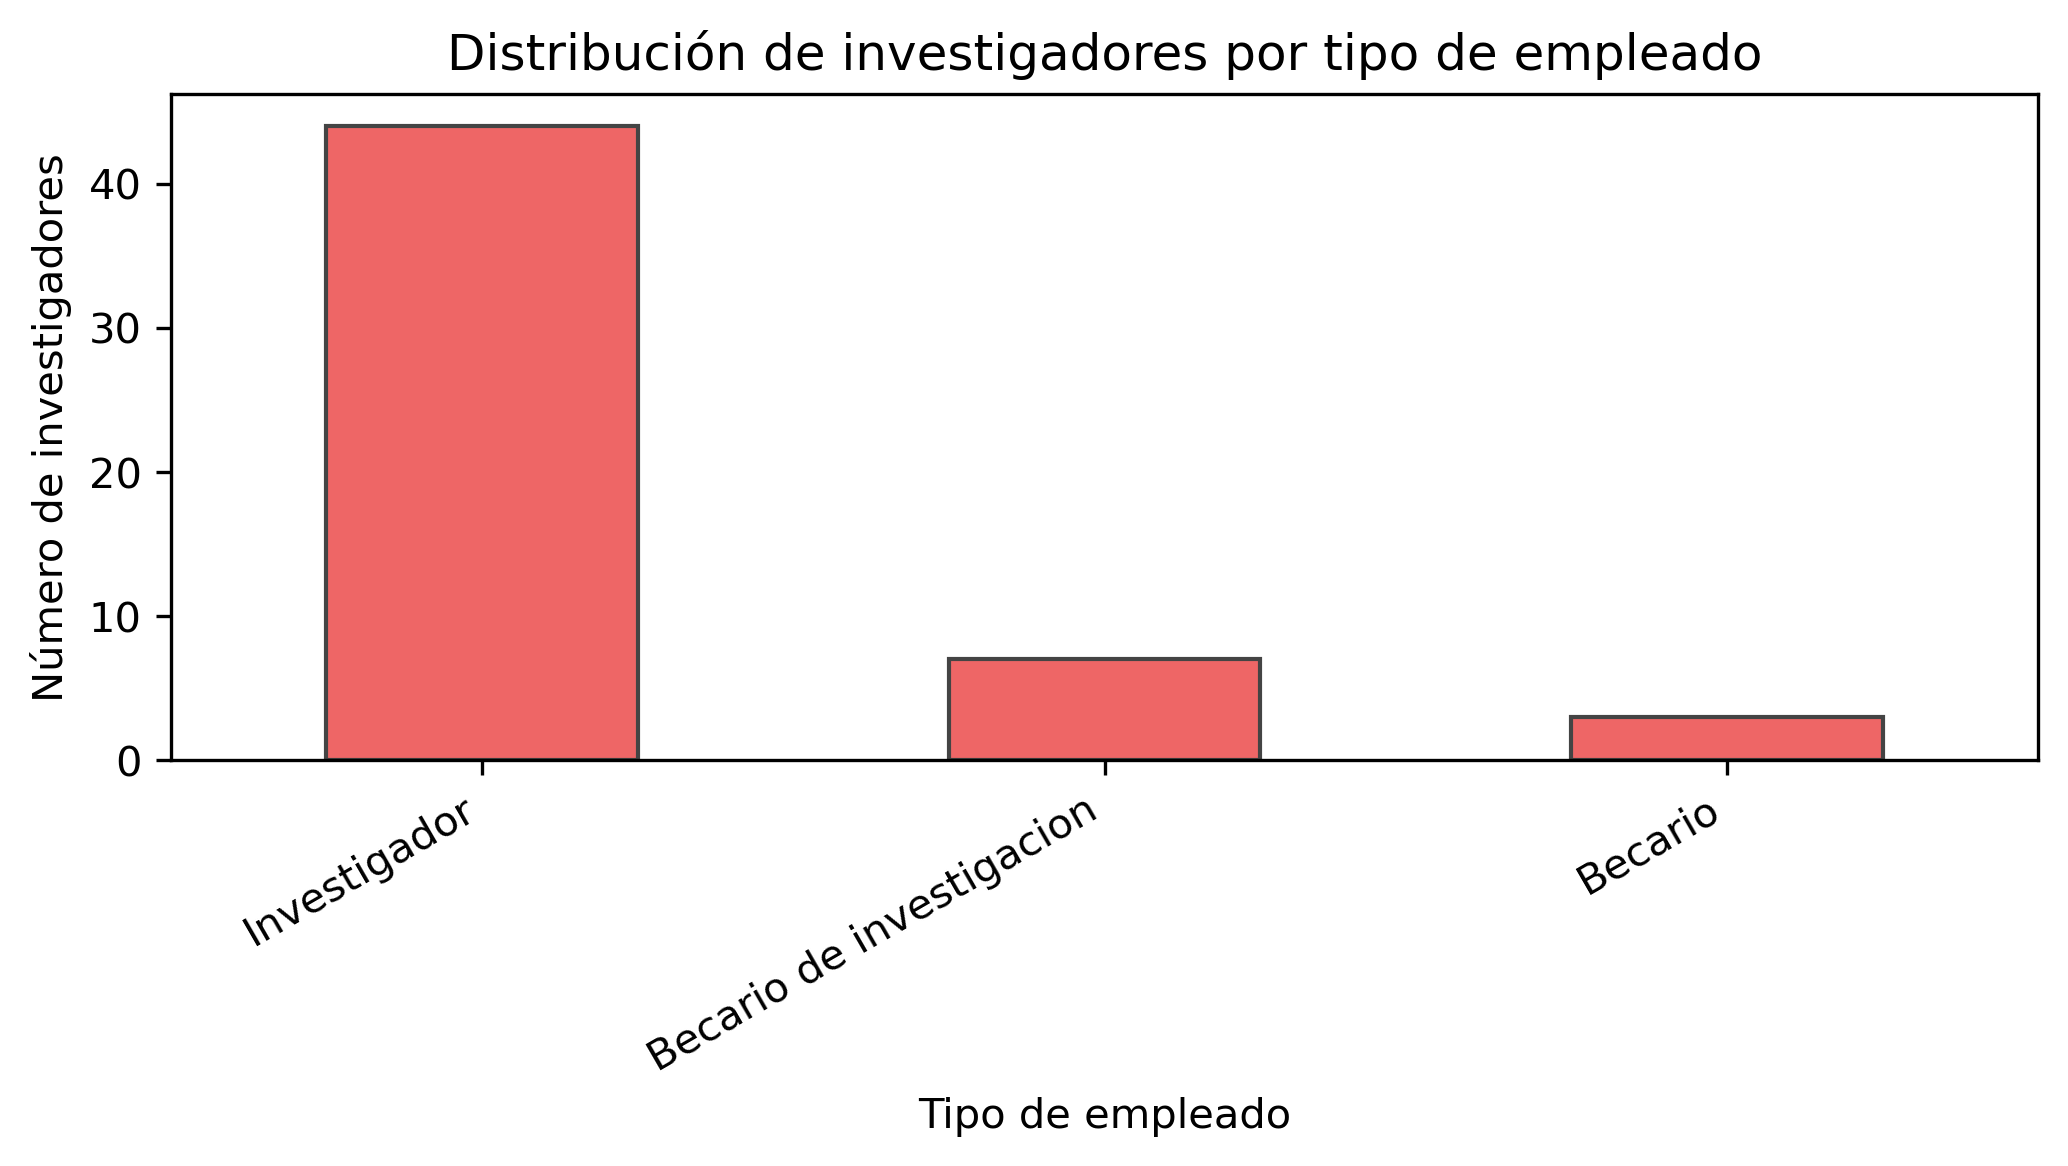
\includegraphics[width=0.7\textwidth]{imgs/eda_tipo_empleado.png}
\caption{Distribución de investigadores por tipo de empleado.}
\label{fig:eda_tipo_empleado}
\end{figure}

La distribución por áreas de trabajo se presenta en la Figura~\ref{fig:eda_areas_trabajo}. En este caso, el gráfico representa asociaciones investigador-área, no una partición estricta de los investigadores, ya que una misma persona puede aparecer vinculada a más de un área. Las áreas con mayor número de asociaciones son Matemática aplicada y Análisis, seguidas por Ciencia de Datos y Becarios.

\begin{figure}[H]
\centering

\includegraphics[width=0.6\textwidth]{imgs/eda_areas_trabajo.png}
\caption{Distribución de asociaciones investigador-área por área de trabajo.}
\label{fig:eda_areas_trabajo}
\end{figure}

\subsection{Artículos y revistas}

En relación con la producción académica recopilada, la Figura~\ref{fig:eda_articulos_revistas} muestra la relación entre el número de artículos asociados a cada investigador y el número de revistas distintas en las que aparecen dichos artículos. En términos generales, se observa una relación creciente entre ambas variables: los investigadores con mayor número de artículos tienden también a estar asociados a un mayor número de revistas. No obstante, la dispersión de los puntos muestra que esta relación no es completamente uniforme, ya que existen diferencias en la concentración de revistas asociadas a cada investigador.

\begin{figure}[H]
\centering
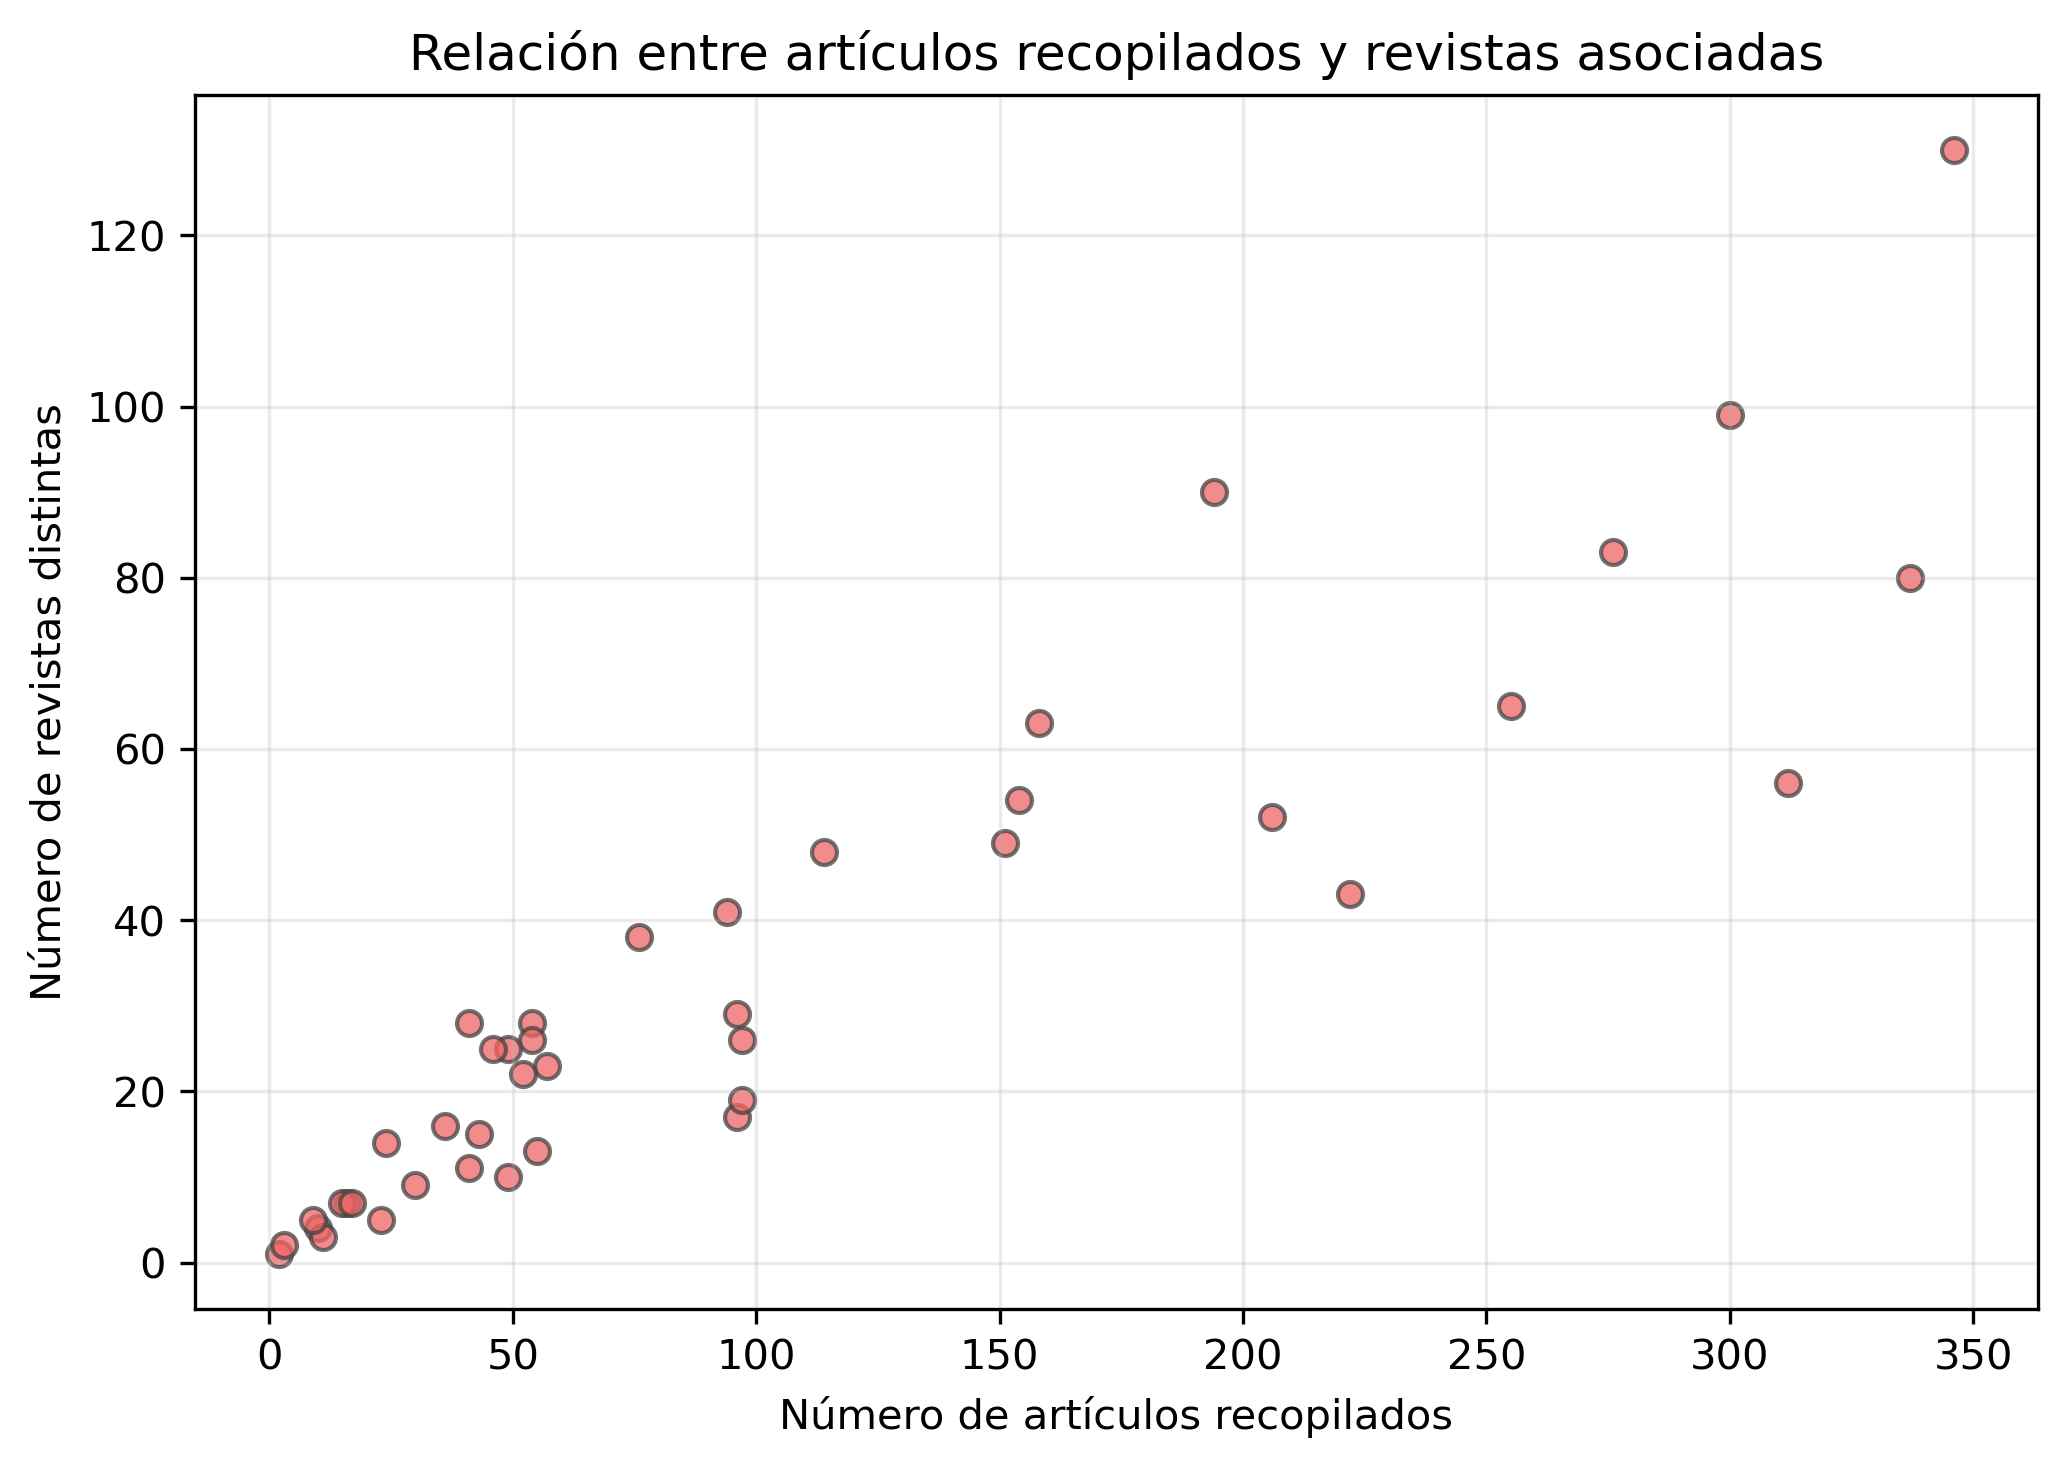
\includegraphics[width=0.6\textwidth]{imgs/eda_articulos_vs_revistas.png}
\caption{Relación entre artículos recopilados y revistas distintas asociadas por investigador.}
\label{fig:eda_articulos_revistas}
\end{figure}

Además de analizar la relación entre artículos y revistas, se revisó la distribución de las revistas según su editorial. La Figura~\ref{fig:eda_top_editoriales} muestra las quince editoriales con mayor número de revistas dentro de la base de datos. Se observa que Elsevier y Springer concentran una parte destacada de las revistas recopiladas, seguidas a mayor distancia por editoriales como MDPI y Taylor \& Francis.

\begin{figure}[H]
\centering
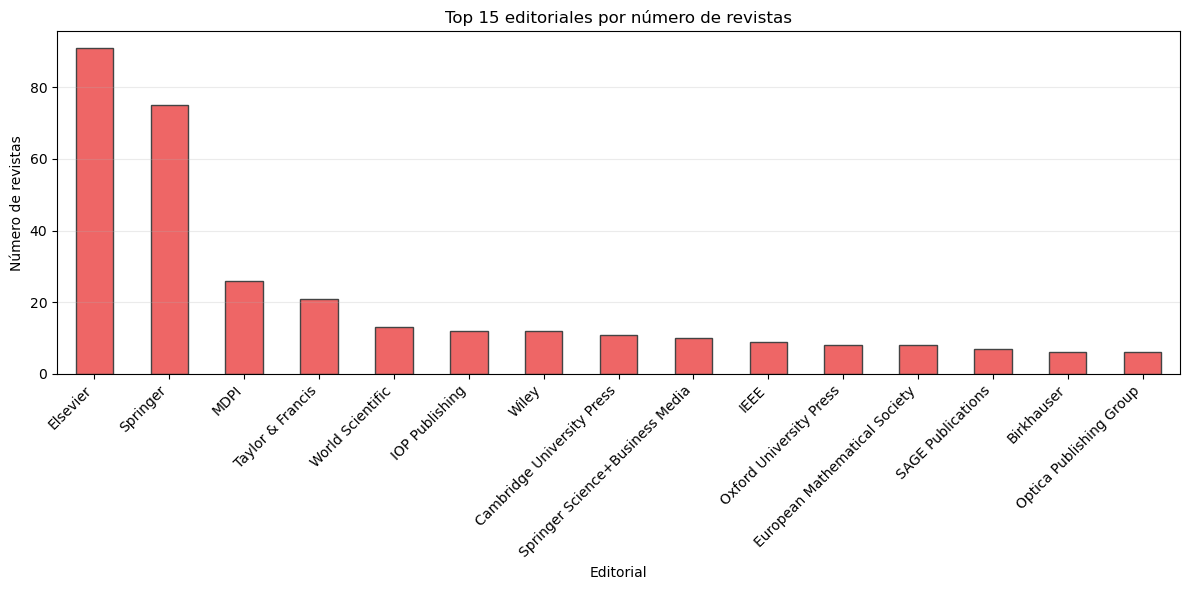
\includegraphics[width=0.9\textwidth]{imgs/eda_top_editoriales.png}
\caption{Principales editoriales asociadas a las revistas recopiladas.}
\label{fig:eda_top_editoriales}
\end{figure}

Esta distribución permite describir la composición de la entidad revista y comprobar que la base recoge publicaciones procedentes de editoriales científicas diversas. No obstante, el gráfico debe interpretarse únicamente como una descripción agregada de la base de datos, no como una valoración de la calidad de las revistas ni de la producción de los investigadores.

\subsection{Actividad en proyectos de investigación}

Para comparar las principales dimensiones de información asociadas a cada investigador, la Figura~\ref{fig:eda_distribuciones_investigador} resume la variabilidad de la información asociada a cada investigador. Los diagramas de caja muestran que el número de artículos y revistas recopilados presenta una dispersión elevada: la mayoría de investigadores se concentra en valores moderados, mientras que algunos casos alcanzan valores considerablemente superiores. En cambio, los proyectos asociados presentan una distribución más compacta. Esta diferencia refleja que la cobertura de publicaciones y revistas es más variable entre investigadores que la información relativa a proyectos, por lo que los resultados derivados de la base deben interpretarse teniendo en cuenta esta heterogeneidad.

\begin{figure}[H]
\centering
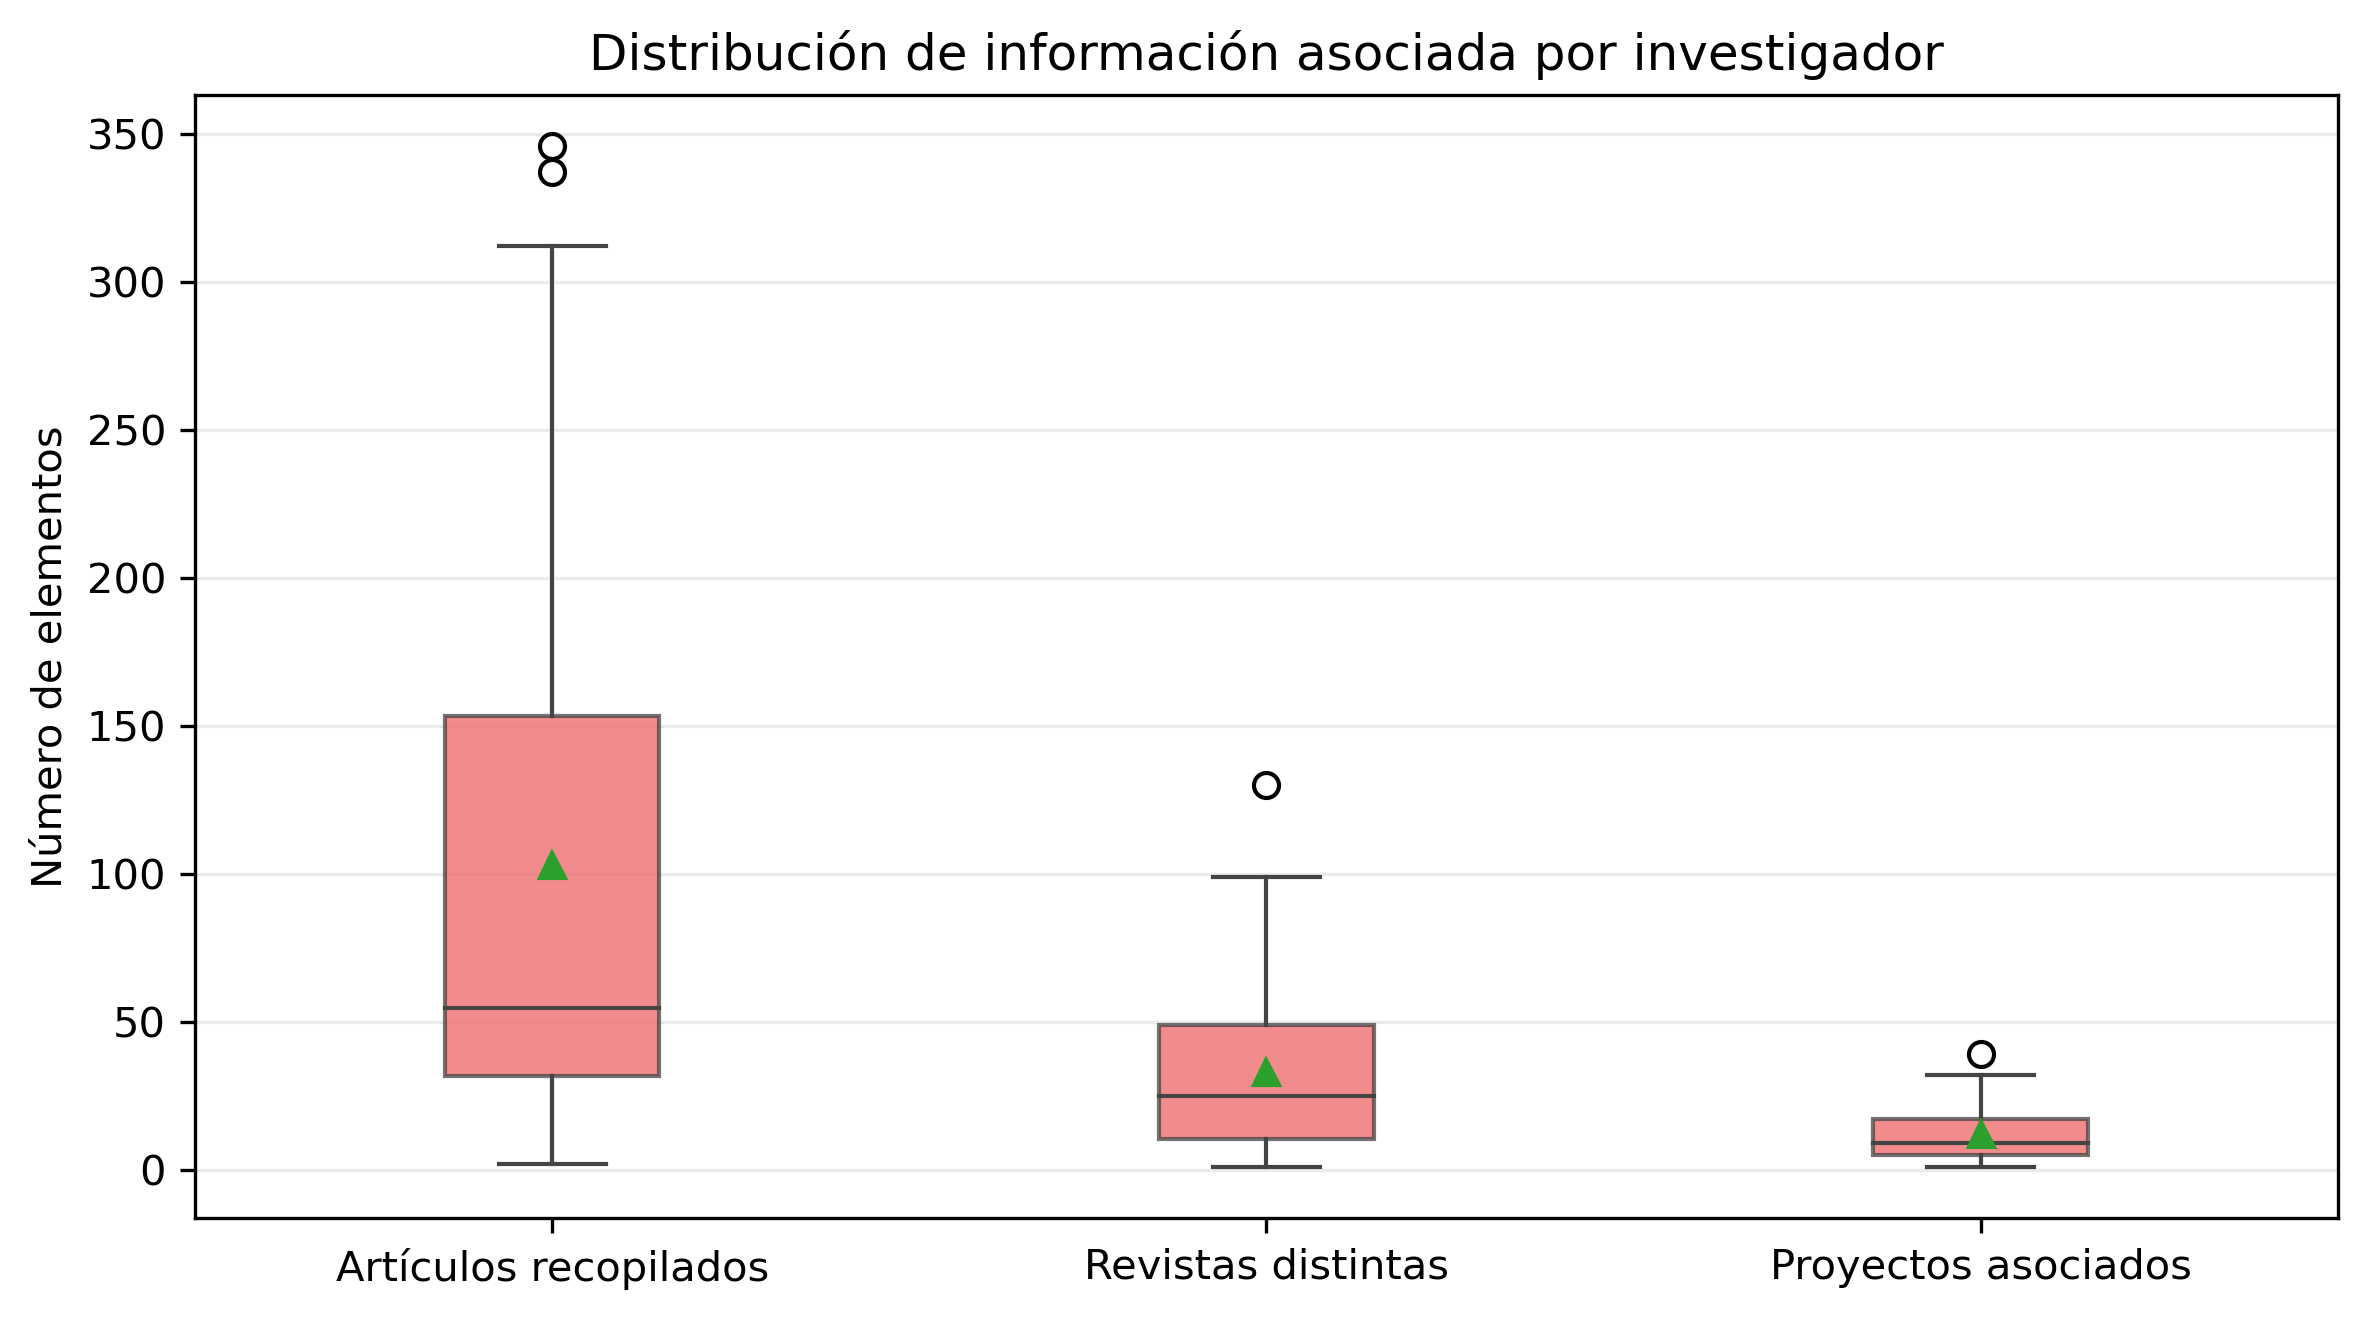
\includegraphics[width=0.7\textwidth]{imgs/eda_distribuciones_por_investigador.png}
\caption{Distribución de artículos, revistas distintas y proyectos asociados por investigador.}
\label{fig:eda_distribuciones_investigador}
\end{figure}

En los proyectos, se analizó cuántos investigadores internos del IUMPA estaban asociados a cada proyecto registrado. La Figura~\ref{fig:eda_investigadores_proyecto} muestra que la mayoría aparecen vinculados a un único investigador interno, aunque esto no implica que sean proyectos individuales, ya que el conteo no incluye participantes externos ni investigadores fuera del alcance del modelo. En concreto, 163 proyectos están asociados a un solo investigador interno del IUMPA, 54 a dos, 31 a tres, 26 a entre cuatro y cinco, 6 a entre seis y diez, y solo uno a más de diez. Esta distribución permite observar la presencia interna del IUMPA en los proyectos recopilados y detectar aquellos casos en los que varios miembros del instituto coinciden en un mismo trabajo.

\begin{figure}[H]
\centering
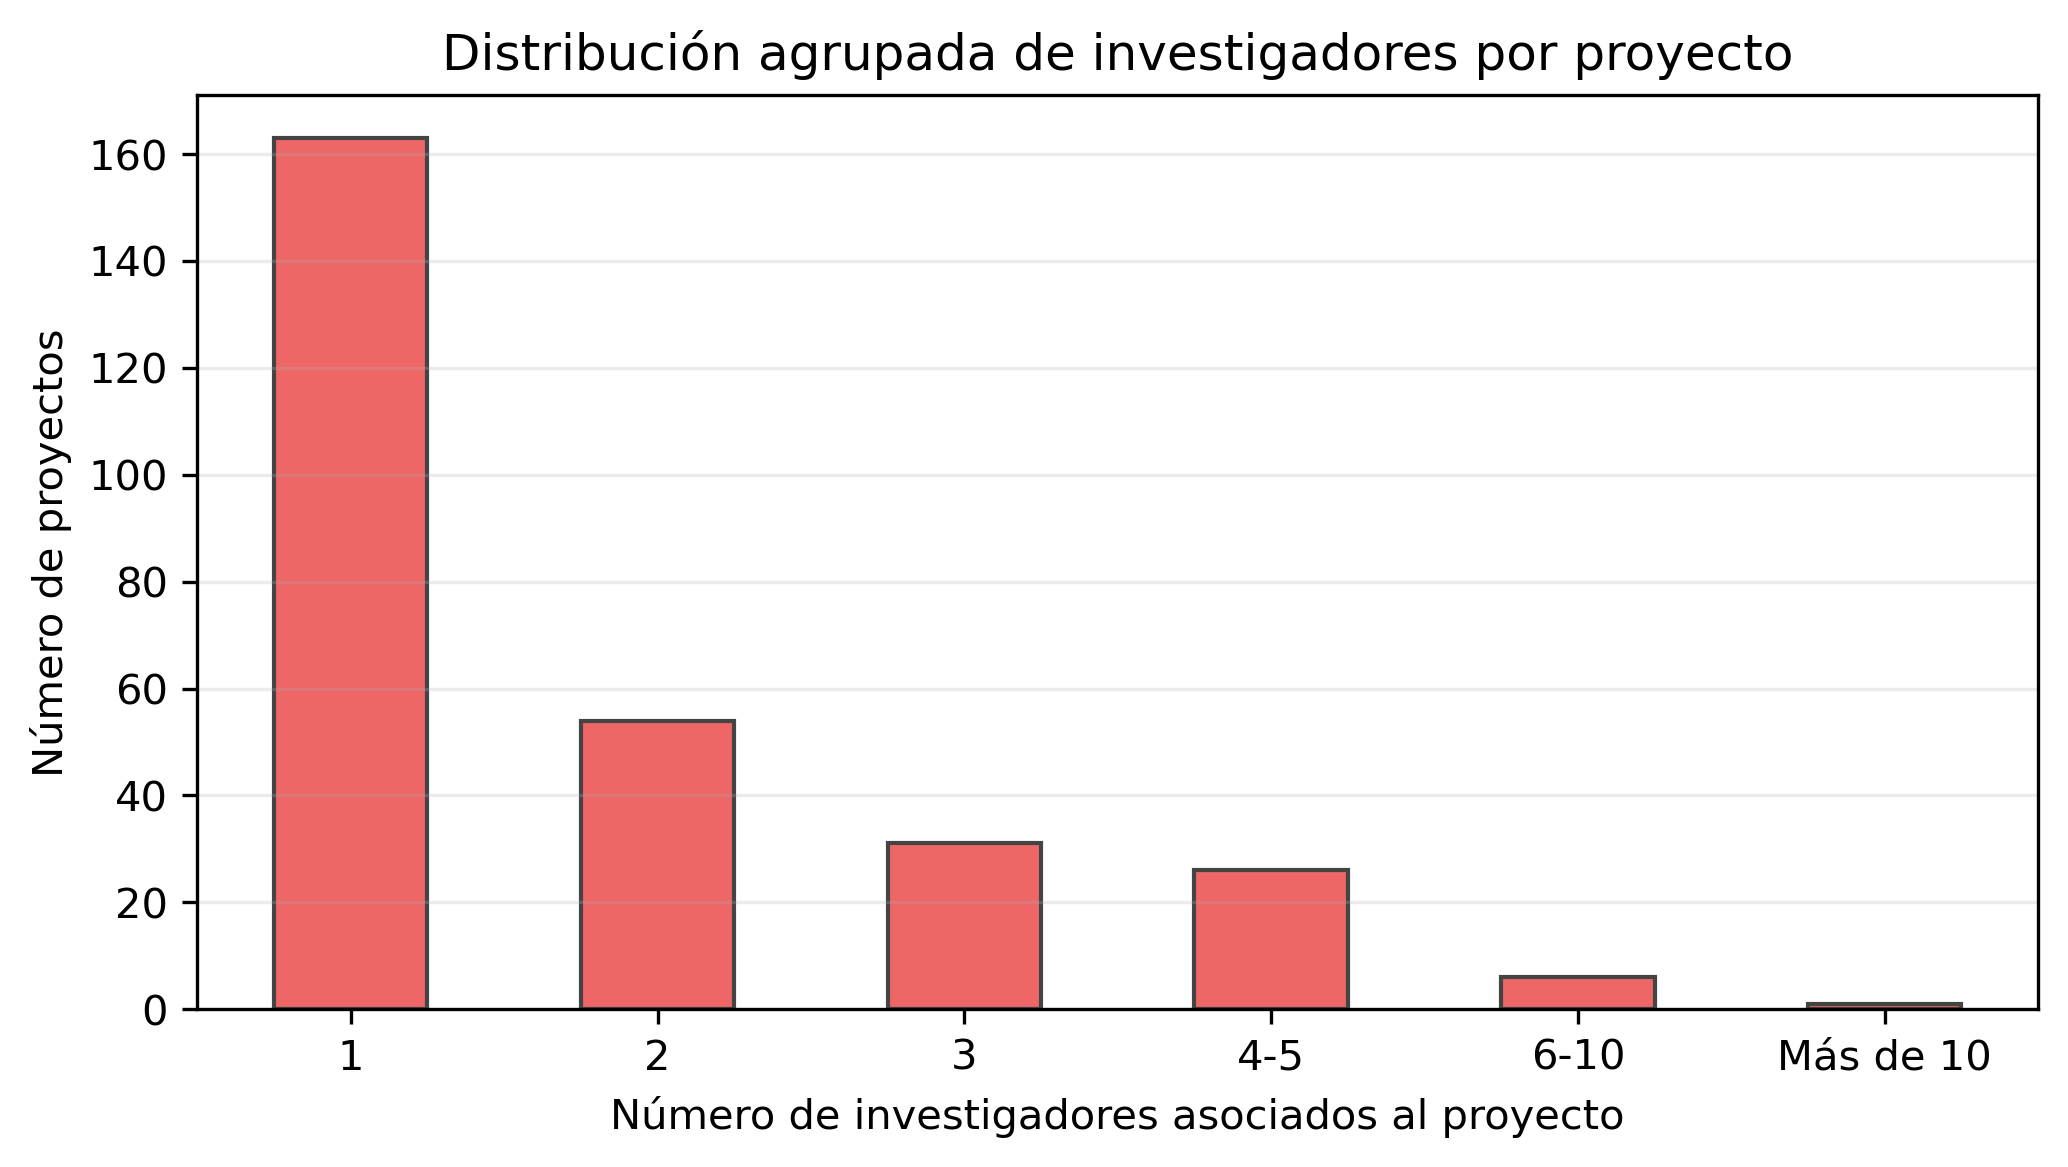
\includegraphics[width=0.6\textwidth]{imgs/eda_investigadores_por_proyecto_agrupado.png}
\caption{Distribución agrupada del número de investigadores internos del IUMPA asociados a cada proyecto.}
\label{fig:eda_investigadores_proyecto}
\end{figure}

Además de analizar cuántos investigadores internos aparecen asociados a cada proyecto, se revisó la distribución temporal de los proyectos recopilados. La Figura~\ref{fig:eda_proyectos_anio} muestra el número de proyectos únicos registrados por año, lo que permite observar cómo se distribuye esta información a lo largo del periodo cubierto por la base de datos.

\begin{figure}[H]
\centering
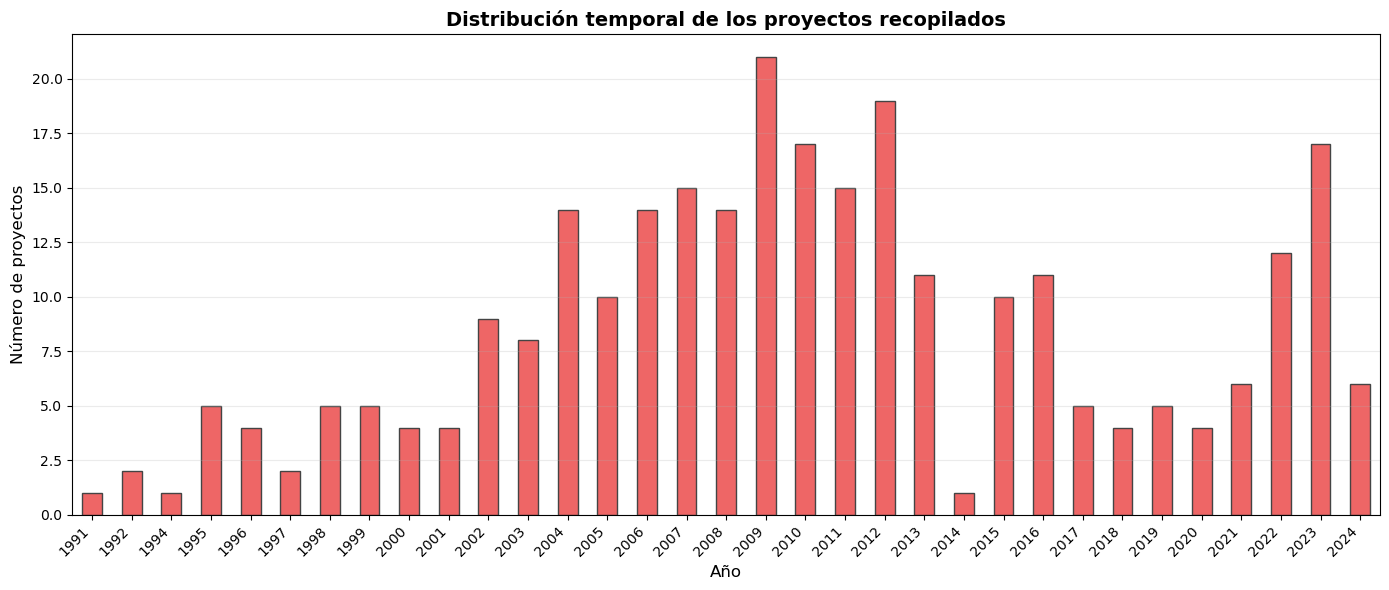
\includegraphics[width=\textwidth]{imgs/distr_temporal_proyectos.png}
\caption{Distribución temporal de los proyectos asociados a investigadores del IUMPA.}
\label{fig:eda_proyectos_anio}
\end{figure}

La distribución muestra una mayor concentración de proyectos en determinados periodos, especialmente alrededor de los años 2009, 2010 y 2012, así como un nuevo incremento en los años más recientes. Esta visualización complementa el análisis anterior, ya que permite describir no solo cuántos proyectos se han recopilado y cuántos investigadores internos aparecen vinculados a ellos, sino también cómo se reparte temporalmente la información disponible.

\subsection{Cobertura de la información temática}

Finalmente, la parte semántica de la base de datos también presenta una cobertura suficiente para servir como punto de partida al análisis posterior. A partir de las revistas recopiladas se construyeron estructuras auxiliares basadas en palabras clave, cuyos principales valores se resumen en la Tabla~\ref{tab:cobertura_semantica}.

\begin{table}[H]
\centering
\small
\begin{tabular}{lr}
\toprule
\textbf{Elemento} & \textbf{Valor} \\
\midrule
Palabras clave únicas & 103 \\
Revistas con representación temática & 643 \\
Investigadores con representación temática & 42 \\
Relaciones investigador-palabra clave activas & 1916 \\
Relaciones revista-palabra clave activas & 4410 \\
\bottomrule
\end{tabular}
\caption{Cobertura de las estructuras semánticas generadas.}
\label{tab:cobertura_semantica}
\end{table}

Estos valores indican que las estructuras semánticas generadas ofrecen cobertura suficiente para construir las representaciones temáticas utilizadas en el análisis posterior.

\section{Valoración de la base de datos construida}

La valoración de la base de datos construida debe hacerse desde su función dentro del proyecto y desde su utilidad como recurso reutilizable. Su principal aportación no reside únicamente en reunir información procedente de distintas fuentes, sino en haberla organizado de forma que pudiera ser utilizada posteriormente para la visualización interactiva, para el análisis semántico y para posibles consultas, actualizaciones o ampliaciones futuras por parte del IUMPA.

Desde el punto de vista del modelo, la estructura final resultó adecuada para los objetivos planteados, ya que permitió representar entidades como investigadores, revistas, áreas y proyectos, así como relaciones derivadas de publicaciones, participación en proyectos y colaboraciones. De este modo, la base de datos se consolidó como una estructura preparada para generar los grafos interactivos y para consultar la actividad investigadora del IUMPA desde una perspectiva relacional.

Además, la información de revistas permitió construir estructuras auxiliares basadas en palabras clave, orientadas a representar temáticamente a los investigadores. Por tanto, esta base de datos también ofrecía un punto de partida adecuado para abordar el análisis semántico desarrollado en la segunda parte del trabajo.

No obstante, su interpretación debe realizarse teniendo en cuenta las limitaciones propias del proceso de recopilación. La información procedía de fuentes públicas con distintos formatos, niveles de detalle y grados de completitud, por lo que la ausencia de un registro no debe interpretarse necesariamente como ausencia de actividad investigadora. En este sentido, la base construida debe entenderse como una estructura útil y ampliable, pero condicionada por la información disponible y por las decisiones de depuración adoptadas durante el proyecto.

Finalmente, dado que la base de datos puede servir como punto de partida para futuras consultas, actualizaciones o ampliaciones, resulta necesario documentar su estructura de forma clara. Por ello, el Apéndice~\ref{ap:diccionario_datos} recoge una descripción de los principales ficheros generados, sus atributos más relevantes y algunos ejemplos visuales de su organización.

%%%%%%%%%%%%%%%%%%%%%%%%%%%%%%%%%%%%%%%%%%%%%%%%%%%%%%%%%%%%%%%%%%%%%%%%%%%%%%%

%%%%%%%%%%%
%Capítulo 5
%%%%%%%%%%%

\chapter{Desarrollo de la aplicación interactiva}

La base de datos construida proporcionaba una estructura organizada de la información, pero su consulta mediante ficheros tabulares no permitía aprovechar la dimensión relacional del proyecto. Para interpretar de forma más intuitiva las relaciones entre investigadores, revistas y proyectos, así como las colaboraciones recogidas en la base de datos, era conveniente trasladar esa información a un entorno visual e interactivo.

Por este motivo, se desarrolló una aplicación interactiva en R mediante Shiny \cite{shiny}. La herramienta permitió convertir las entidades y relaciones definidas previamente en grafos explorables, de forma que el usuario pudiera consultar visualmente la estructura de la información sin necesidad de acceder directamente a los ficheros de datos.

La aplicación se organizó en torno a distintos grafos interactivos, cada uno orientado a representar una parte concreta de la información recopilada. Su desarrollo implicó definir la estructura general de la herramienta, transformar los datos tabulares en nodos y relaciones visuales, e incorporar elementos de interacción que facilitaran la exploración de la información.

\section{Diseño general de la herramienta}

La aplicación se estructuró como una herramienta desarrollada en R mediante Shiny, organizada a partir de la separación entre la lectura de datos, el procesamiento de la información y la generación de componentes visuales. Esta organización permitió mantener una correspondencia clara entre los ficheros de la base de datos y los grafos mostrados al usuario.

De esta forma, la herramienta puede entenderse a partir de tres fases principales:

\begin{itemize}
    \item \textbf{Fase de lectura de los ficheros}: en la que se cargaban las entidades y relaciones necesarias para construir las visualizaciones.

    \item \textbf{Lógica de procesamiento}: encargada de adaptar esos datos al formato requerido por los grafos, diferenciando los elementos que debían representarse como nodos y las conexiones que debían representarse como enlaces.

    \item \textbf{Interfaz visual}: destinada a consultar los grafos resultantes y acceder a la información asociada a los elementos representados.
\end{itemize}

Los ficheros construidos previamente actuaban como entrada del sistema, mientras que la aplicación se encargaba de interpretarlos y convertirlos en representaciones visuales interactivas. De este modo, los cambios en los datos podían incorporarse con mayor facilidad, siempre que se mantuviera la estructura esperada por la herramienta.

El diseño de la aplicación estuvo condicionado por el objetivo exploratorio del proyecto. No se buscaba construir una plataforma cerrada de consulta estadística, sino una herramienta que permitiera navegar por la información recopilada y observar las relaciones existentes entre investigadores, revistas y proyectos, así como las colaboraciones derivadas de publicaciones y proyectos compartidos. Además, se incorporó la posibilidad de filtrar las visualizaciones por áreas de trabajo, utilizando la relación previamente definida entre investigadores y áreas. Por ello, la organización general de la herramienta se orientó a facilitar una exploración visual progresiva, desde una visión global de las relaciones hasta la consulta de información concreta asociada a cada elemento.

Desde el punto de vista de implementación, la aplicación siguió la estructura habitual de Shiny, separando la definición de la interfaz de usuario de la lógica encargada de procesar los datos y generar las visualizaciones. Esta separación facilitó mantener diferenciadas la parte visual de la aplicación y la lógica encargada de preparar los datos para su representación gráfica.

\section{Construcción de los grafos interactivos}

La construcción de los grafos interactivos consistió en transformar las entidades y relaciones de la base de datos en estructuras visuales formadas por nodos y enlaces. Los nodos representaban los elementos del sistema que se querían visualizar, mientras que los enlaces indicaban las relaciones existentes entre ellos. De esta forma se transformaron los ficheros tabulares descritos anteriormente en visualizaciones orientadas a explorar la actividad investigadora del IUMPA.

El proceso seguido para construir cada grafo mantuvo una lógica común. En primer lugar, se seleccionaban los ficheros necesarios para cada visualización. A partir de ellos se identificaban los elementos que debían representarse como nodos y las conexiones que debían convertirse en enlaces. Posteriormente, los datos se adaptaban al formato requerido por la librería de visualización utilizada en la aplicación, Apache ECharts \cite{echarts}, incorporando la información necesaria para mostrar etiquetas, categorías y atributos asociados a cada elemento.

En el caso de los investigadores, también se conservó su asociación con las áreas de trabajo, no como nodos independientes del grafo, sino como atributo utilizado posteriormente para filtrar las visualizaciones y para contextualizar la información mostrada al seleccionar un investigador.

Uno de los grafos principales de la aplicación permitió representar la relación entre investigadores y revistas a partir de los artículos recopilados. Esta visualización se construyó a partir de la relación \textit{ha\_publicado\_en}, utilizando como nodos los investigadores y las revistas, y como enlaces las relaciones que conectaban a cada investigador con los medios en los que aparecían sus artículos. En este caso, el grafo permitía observar la distribución de la producción académica recopilada y explorar qué revistas aparecían asociadas a cada investigador.

\begin{figure}[H]
\centering
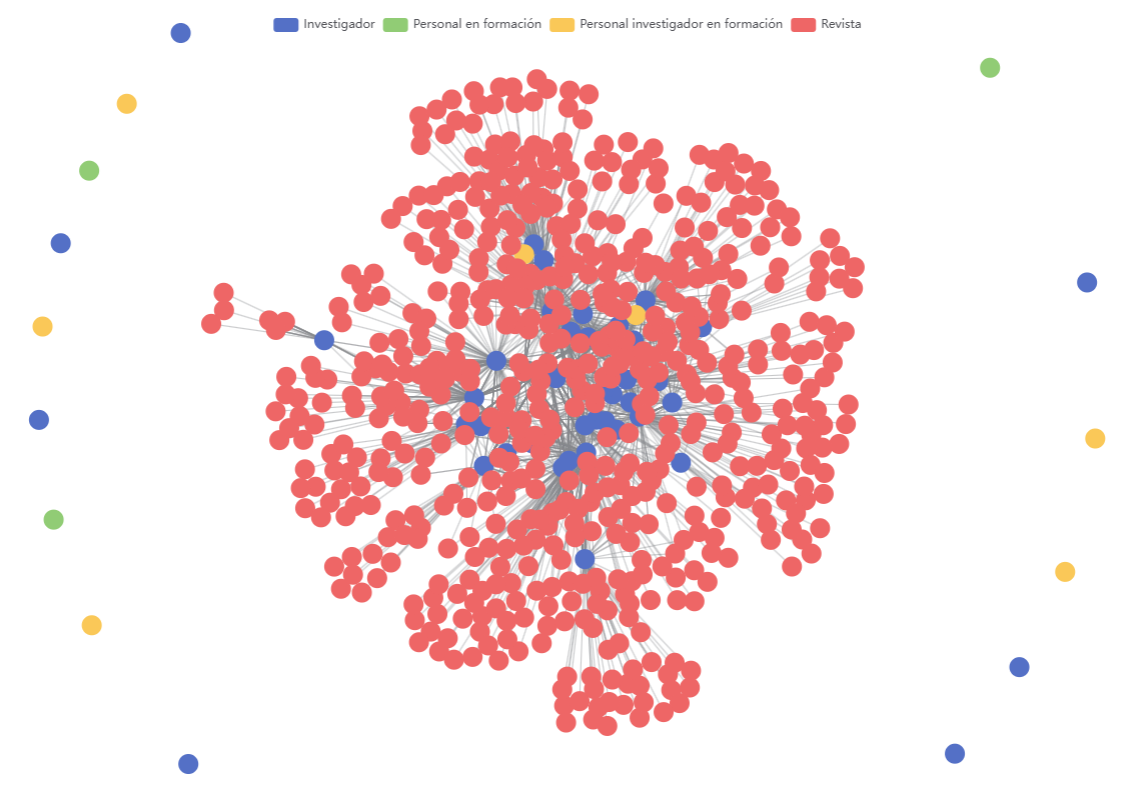
\includegraphics[width=0.8\textwidth]{imgs/inv_vs_revistas.png}
\caption{Grafo de relación entre investigadores y revistas.}
\label{fig:grafo_investigadores_revistas}
\end{figure}

La información relativa a proyectos se representó mediante un grafo específico basado en la relación \textit{ha\_participado\_en}. Esta visualización utilizaba como nodos los investigadores y los proyectos, y como enlaces la participación de cada investigador en los proyectos registrados. Este grafo permitía explorar una dimensión de la actividad investigadora distinta a la derivada de los artículos, identificando qué investigadores aparecían vinculados a proyectos concretos. Para simplificar la visualización, los proyectos se mostraron a partir de su título, de forma que registros con el mismo nombre quedaban consolidados en un único nodo visual.
 
\begin{figure}[H]
\centering
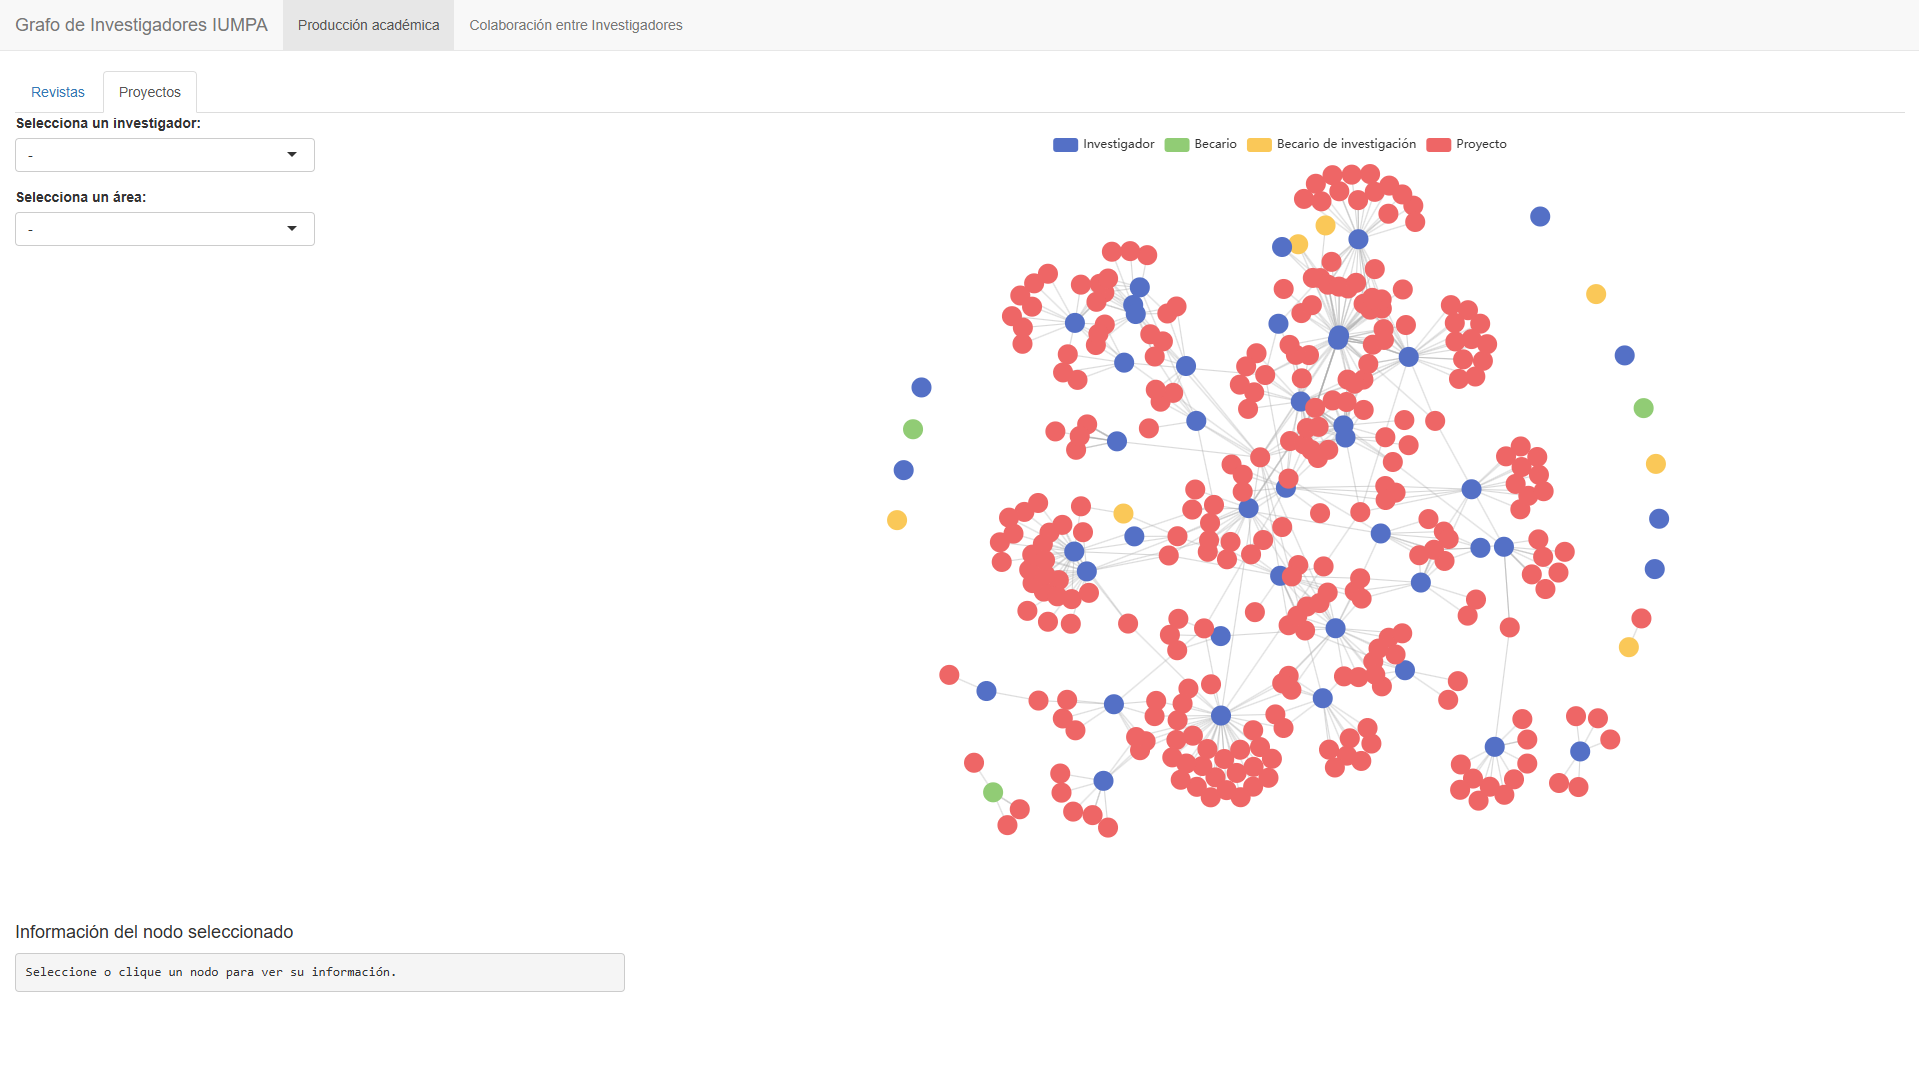
\includegraphics[width=0.8\textwidth]{imgs/inv_vs_proyectos.png}
\caption{Grafo de relación entre investigadores y proyectos de investigación.}
\label{fig:grafo_investigadores_proyectos}
\end{figure}

Además de los grafos que relacionaban investigadores con otros tipos de entidades, la aplicación incorporó visualizaciones centradas en relaciones entre investigadores. A partir de la relación \textit{ha\_publicado\_con}, se construyó un grafo de colaboración basado en artículos compartidos. En este caso, los nodos representaban investigadores y los enlaces indicaban la existencia de publicaciones conjuntas entre ellos. Esta visualización permitía observar relaciones de coautoría y detectar conexiones derivadas de la producción académica recopilada.

\begin{figure}[H]
\centering
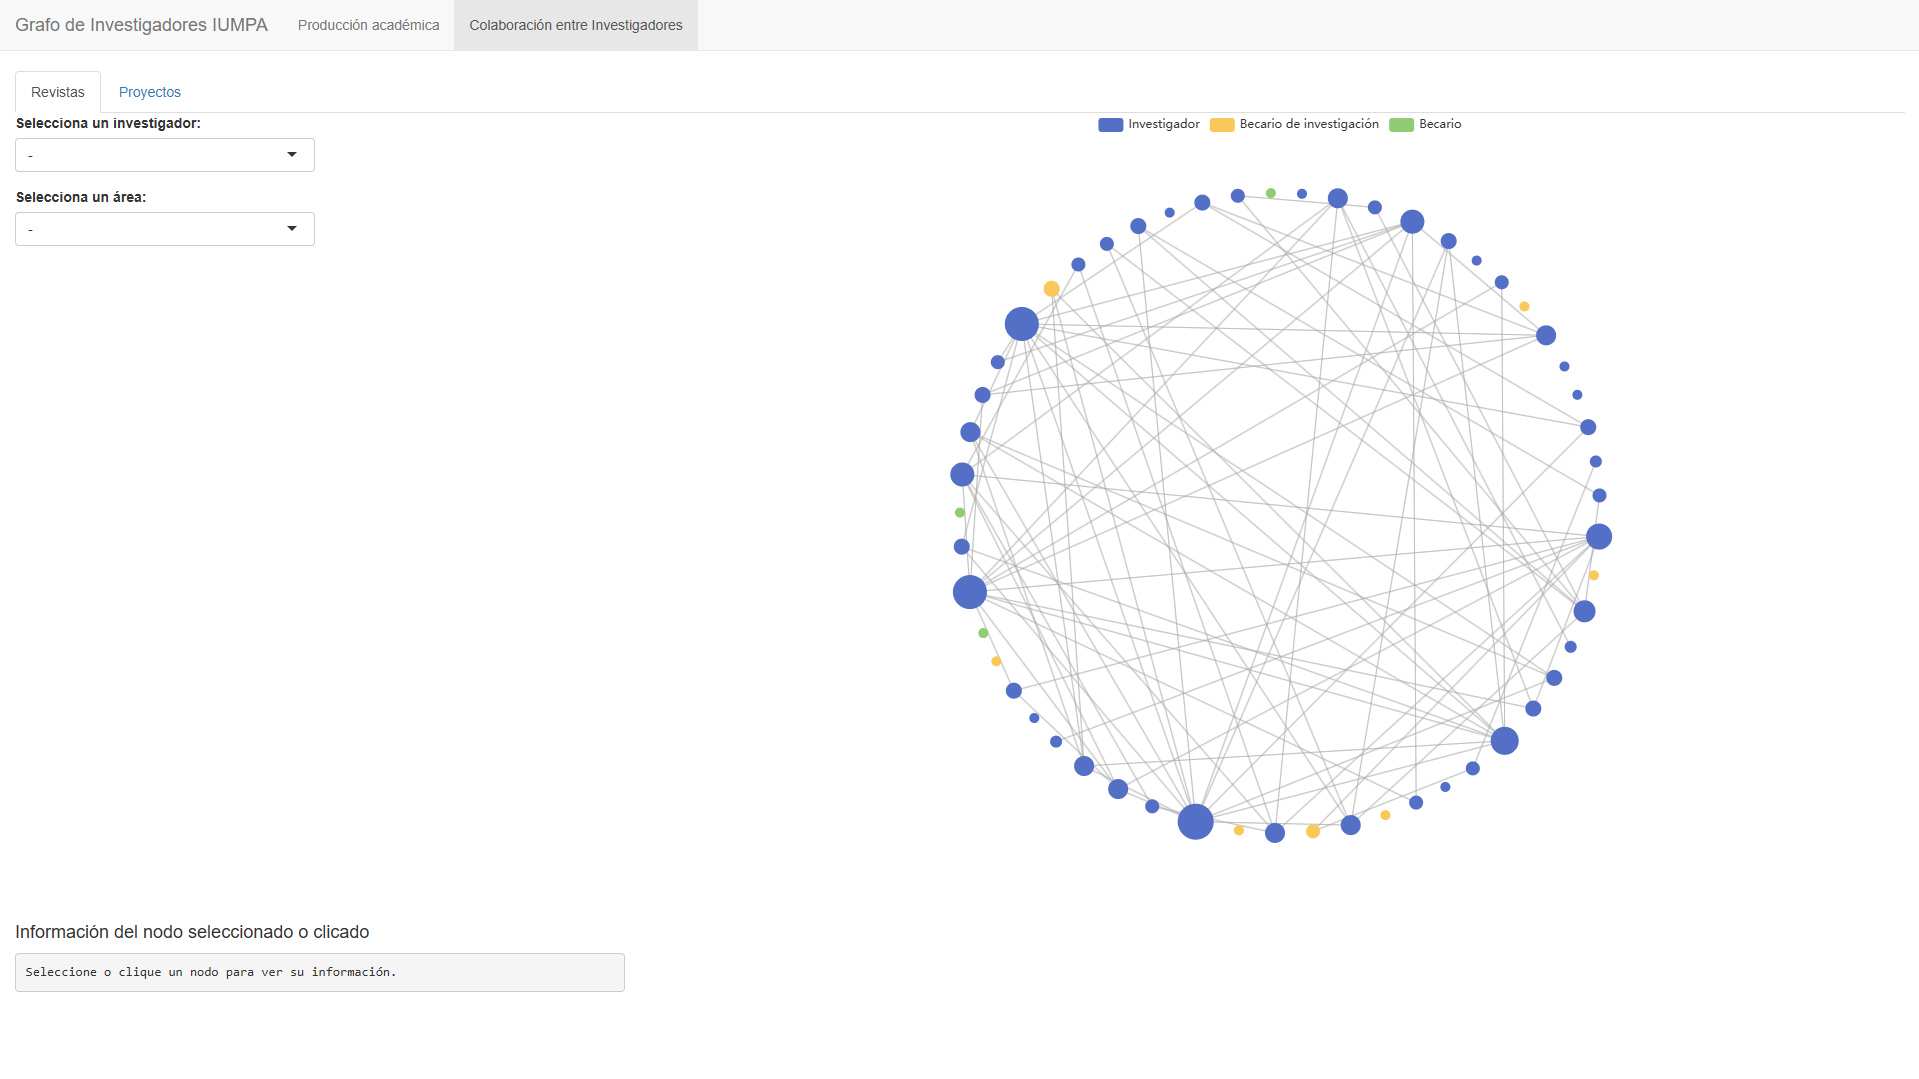
\includegraphics[width=0.8\textwidth]{imgs/inv_vs_inv_revistas.png}
\caption{Grafo de colaboración entre investigadores a partir de artículos compartidos.}
\label{fig:grafo_colaboracion_articulos}
\end{figure}

De forma análoga, la relación \textit{ha\_participado\_con} permitió representar colaboraciones derivadas de la participación conjunta en proyectos. En este grafo, los nodos representaban investigadores y los enlaces indicaban que dos investigadores aparecían asociados a un mismo proyecto. Esta visualización ofrecía una perspectiva complementaria a la colaboración basada en artículos y permitía diferenciar entre relaciones surgidas de la producción académica y relaciones derivadas de la participación común en proyectos de investigación.

En ambos grafos de colaboración entre investigadores, las relaciones se trataron como no dirigidas, ya que la colaboración entre dos personas debía interpretarse de forma simétrica. Esta decisión permitió evitar pérdidas de información cuando una relación aparecía registrada en un único sentido en los ficheros de partida, asegurando que las conexiones representadas reflejaran correctamente la existencia de colaboración entre los investigadores implicados.

\begin{figure}[H]
\centering
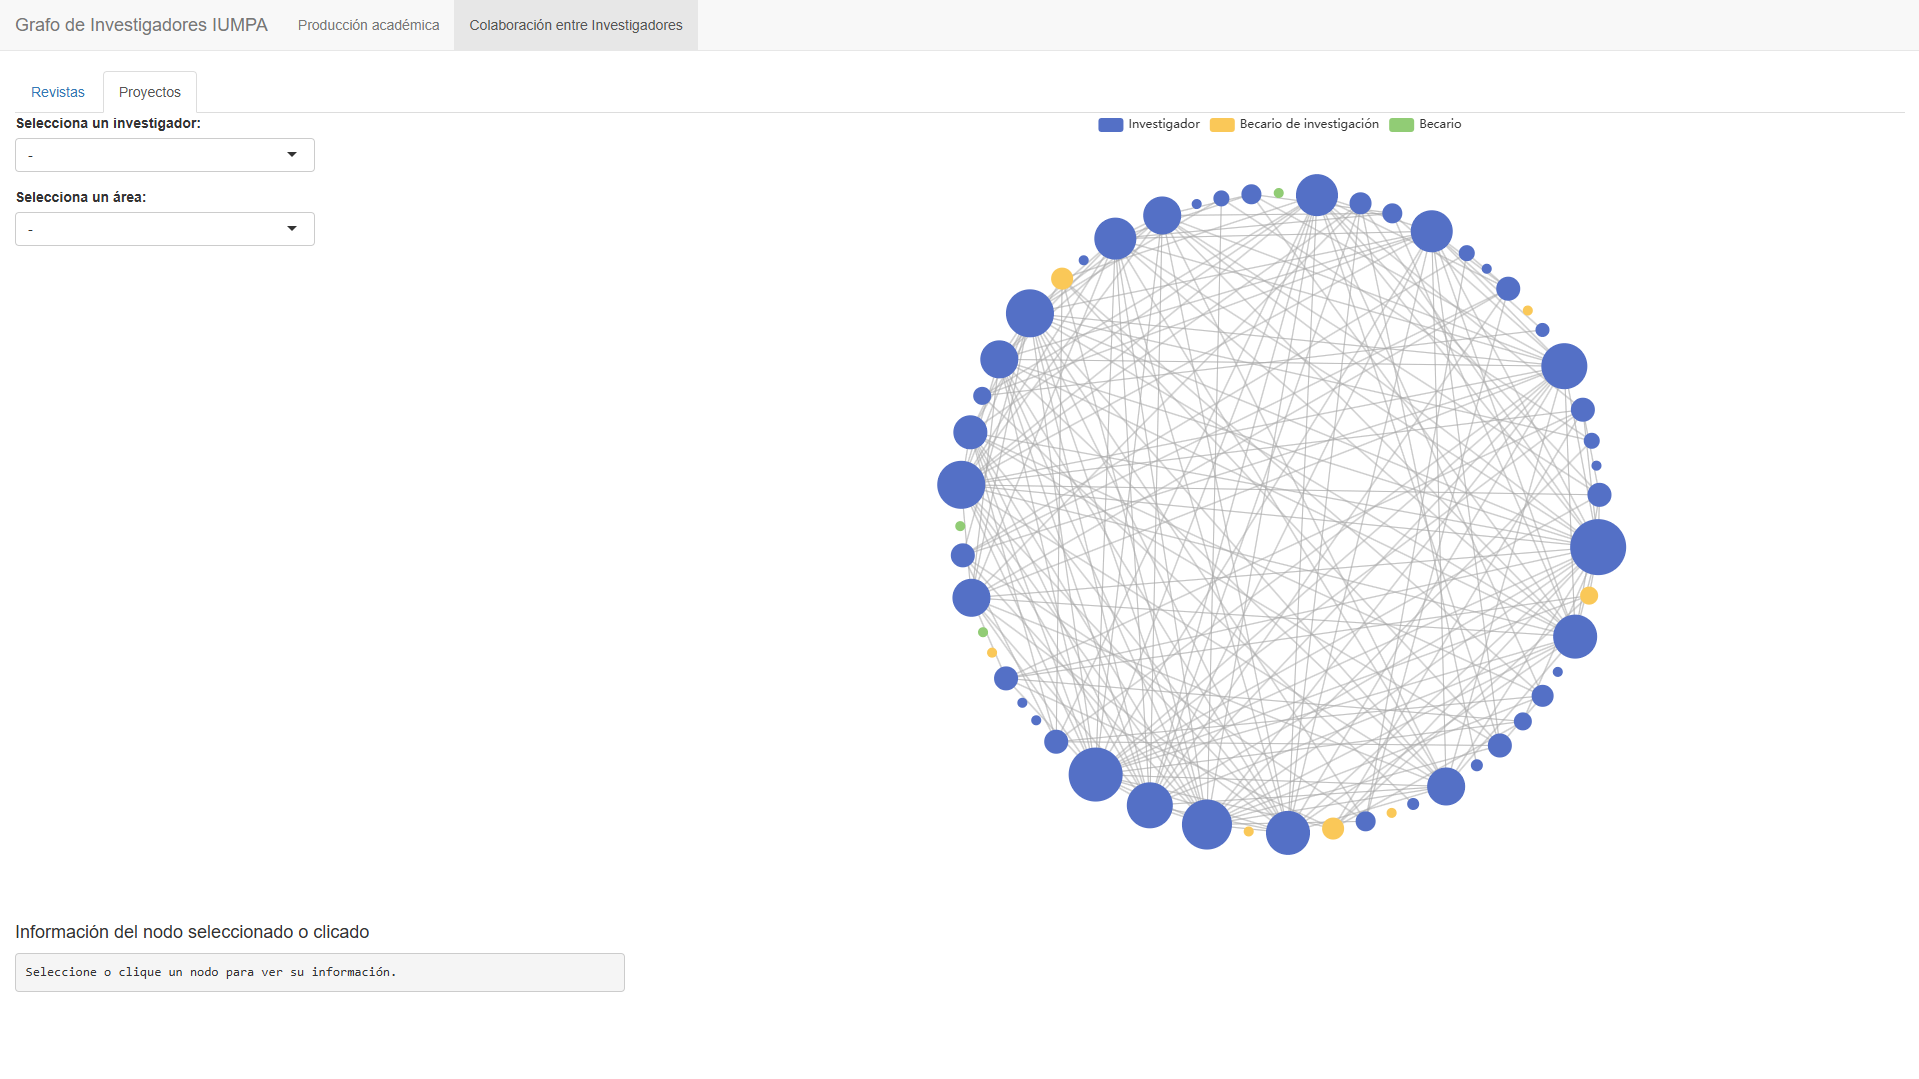
\includegraphics[width=0.8\textwidth]{imgs/inv_vs_inv_proyectos.png}
\caption{Grafo de colaboración entre investigadores a partir de la participación conjunta en proyectos.}
\label{fig:grafo_colaboracion_proyectos}
\end{figure}

La existencia de varios grafos permite evitar una única visualización excesivamente compleja. En lugar de representar todas las entidades y relaciones al mismo tiempo, la aplicación separa la información en vistas específicas: una centrada en la producción académica, otra en la participación en proyectos y otras dos en las relaciones de colaboración entre investigadores. Esta decisión facilita la interpretación de los resultados y permite que el usuario explore la información de forma progresiva.

\section{Elementos de interacción y visualización}

Además de construir los grafos interactivos, la aplicación incorporó distintos elementos de interacción y codificación visual para facilitar su exploración. El objetivo de estos elementos era permitir que el usuario pudiera pasar de una visión general de la red a consultas más concretas sobre los elementos representados, sin necesidad de consultar directamente los ficheros de datos.

Uno de los principales mecanismos de interacción fue el uso de selectores. En los cuatro grafos desarrollados se incorporaron controles que permitían filtrar la visualización por investigador y por área de trabajo, aunque su efecto dependía del tipo de grafo consultado:
\begin{itemize}
    \item \textbf{Producción académica}: el selector de investigador permitía mostrar únicamente las revistas o proyectos asociados a una persona concreta.

    \item \textbf{Colaboración entre investigadores}: permitía centrar la visualización en un investigador y en sus conexiones dentro de la red correspondiente.
\end{itemize}

Por su parte, el filtro por área permitía restringir la visualización a los investigadores asociados a una determinada línea de trabajo, junto con los elementos conectados a ellos cuando corresponda. De esta forma, el usuario podía reducir la complejidad de la red y analizar subconjuntos más manejables de la información.

\begin{figure}[H]
\centering
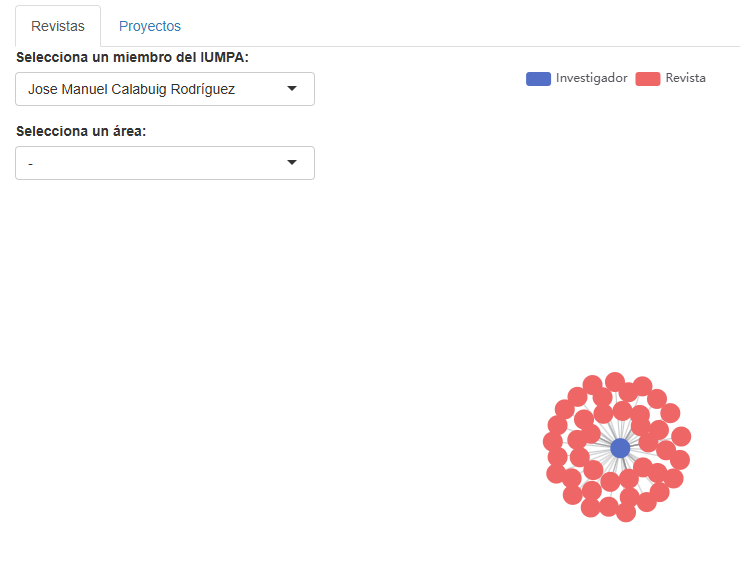
\includegraphics[width=0.48\textwidth]{imgs/filtrado_investigador.png}
\hfill
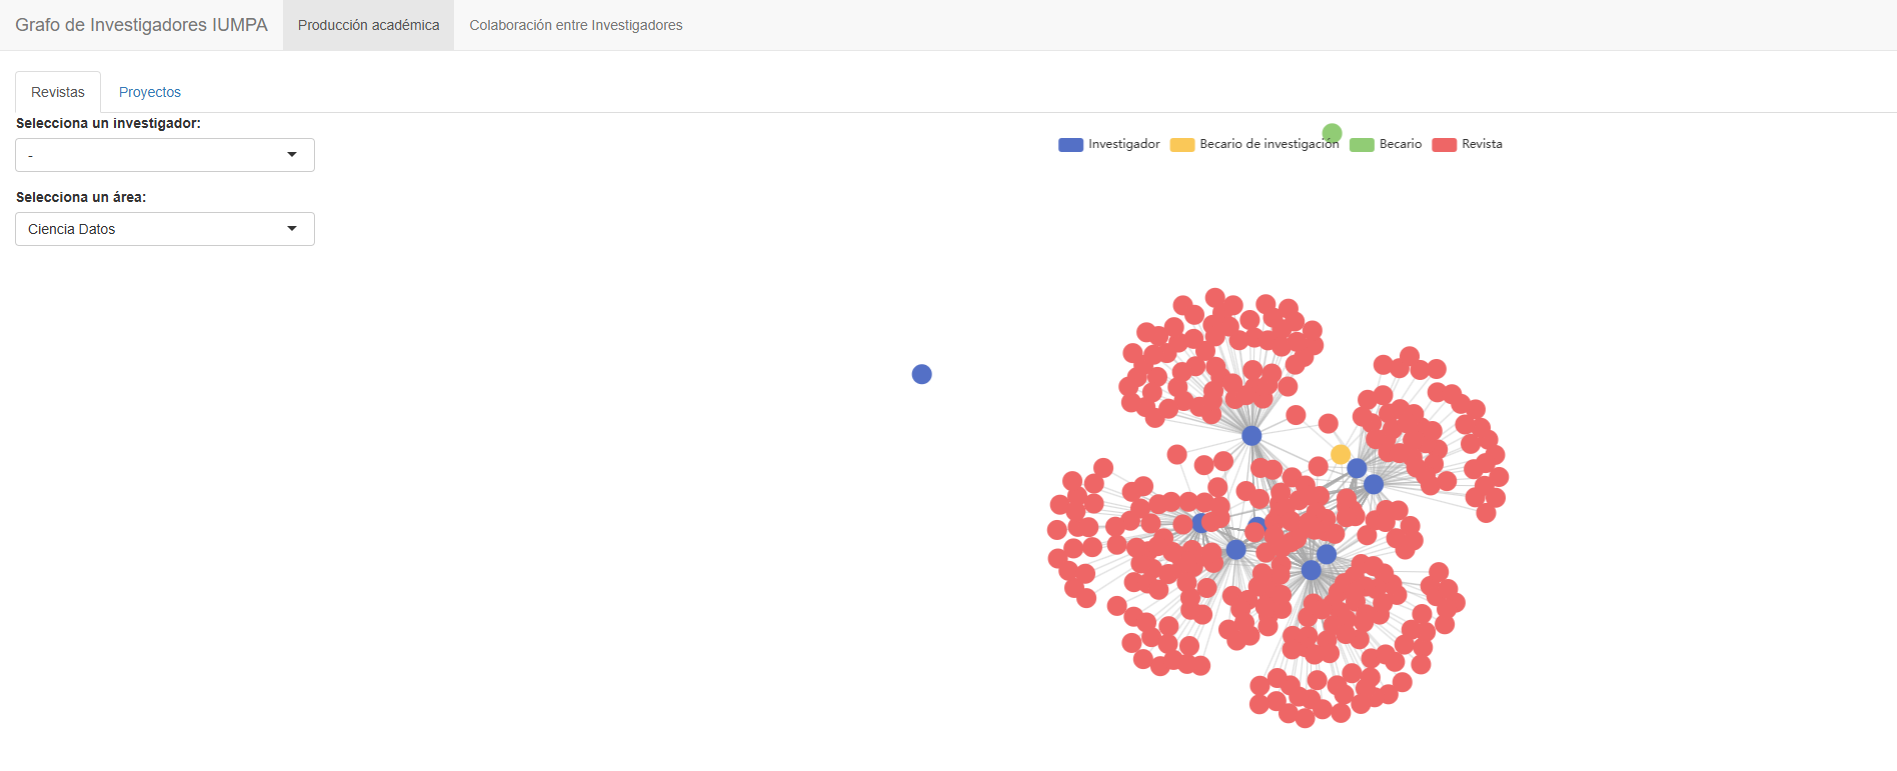
\includegraphics[width=0.48\textwidth]{imgs/filtrado_area.png}
\caption{Ejemplos de filtrado mediante selectores en los grafos interactivos.}
\label{fig:filtros_selectores}
\end{figure}

Además de estos selectores, la leyenda de los grafos también actuaba como un elemento interactivo. Al seleccionar o deseleccionar una categoría de la leyenda, la aplicación permitía ocultar o mostrar los nodos pertenecientes a dicho grupo. Esta funcionalidad resultaba útil para centrar la visualización en determinados tipos de elementos, por ejemplo ocultando algún tipo de personal cuando se quería observar con mayor claridad una parte concreta del grafo.

\begin{figure}[H]
\centering
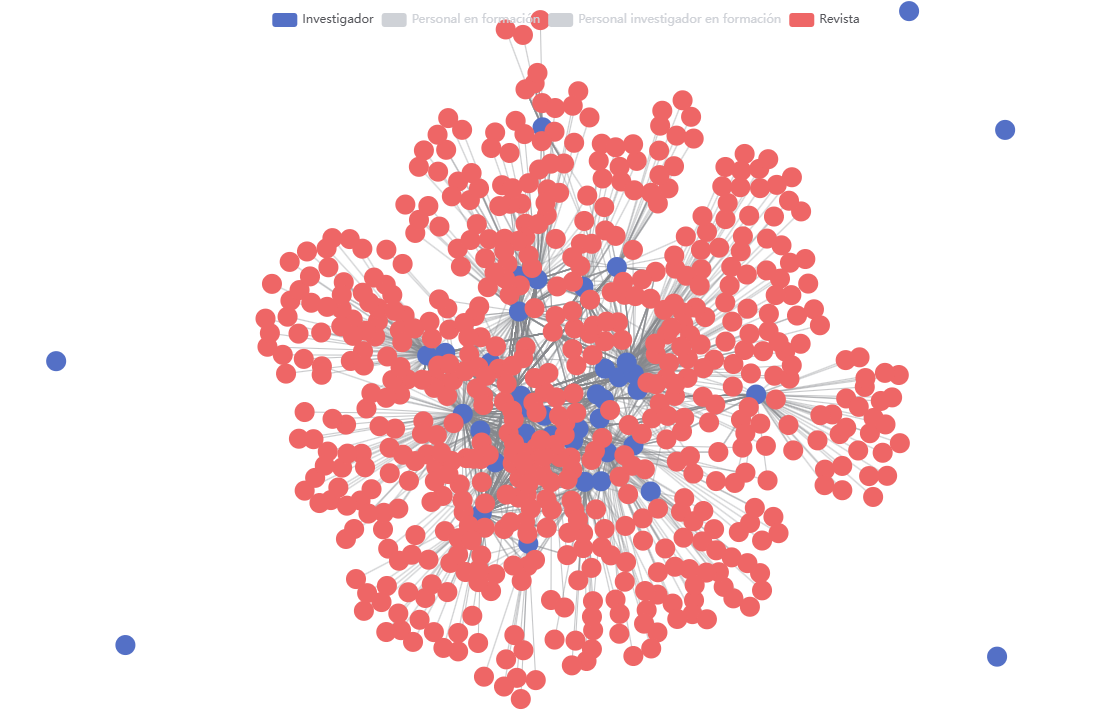
\includegraphics[width=0.95\textwidth]{imgs/filtrado_leyenda.png}
\caption{Ejemplo de filtrado visual mediante la selección de categorías en la leyenda del grafo.}
\label{fig:filtro_leyenda}
\end{figure}

La aplicación también utilizó recursos de codificación visual para facilitar la interpretación de los grafos. En primer lugar, se emplearon colores fijos para diferenciar los tipos de elementos representados. En todos los grafos, los investigadores se muestran en azul, los becarios en verde y los becarios de investigación en amarillo. Además, en los grafos de producción académica, las revistas y los proyectos se representan en rojo. Esta codificación cromática se mantuvo constante entre vistas para que el usuario pudiera interpretar los nodos de forma homogénea al cambiar de grafo.

Junto con el color, en los grafos de colaboración entre investigadores se incorporó una diferencia de tamaño entre nodos. En estas visualizaciones, el tamaño del nodo representaba el número de conexiones del investigador dentro del grafo correspondiente. Por tanto, los nodos de mayor tamaño indicaban investigadores con más conexiones dentro de la red mostrada en cada caso (colaboraciones derivadas de artículos compartidos en un grafo y colaboraciones derivadas de proyectos comunes en el otro). Esta representación añadía una segunda capa de información visual y permitía identificar nodos con mayor conectividad dentro de la red, sin plantear esta información como una métrica individual de productividad.

Además de estos elementos visuales, la exploración de los grafos se apoyó en mecanismos de interacción directa. Al situar el cursor sobre un nodo, la aplicación mostraba información emergente asociada al elemento seleccionado, con diferentes resultados según el grafo: 
\begin{itemize}
    \item \textbf{Investigadores y revistas}: esta información incluía, para los investigadores, el número de revistas asociadas y el número de artículos recopilados, mientras que para las revistas indicaba el número de investigadores vinculados a ellas.

    \item \textbf{Investigadores y proyectos}: la información emergente mostraba, para cada investigador, el número de proyectos asociados y, para cada proyecto, el número de investigadores vinculados.

    \item \textbf{Colaboración entre investigadores}: en ambos casos, esta información permitía consultar el número total de conexiones del investigador dentro de la red mostrada.
\end{itemize}

Asimismo, la interacción con los enlaces permitía interpretar qué elementos quedaban conectados en el grafo, reforzando la lectura de las relaciones visualizadas.

Por otro lado, la selección mediante clic permitía pasar de esta identificación rápida a una consulta más detallada. Al seleccionar un nodo, la aplicación mostraba información específica del elemento seleccionado en un panel informativo, adaptada al tipo de entidad consultada. En todos los grafos, cuando el nodo seleccionado correspondía a un investigador, el panel informativo mostraba en primer lugar su nombre y las áreas de trabajo asociadas. Esta información permitía contextualizar al investigador antes de consultar sus publicaciones, proyectos o relaciones de colaboración.

En los grafos de producción académica, este panel ofrecía distinta información adicional según el tipo de nodo:

\begin{itemize}
    \item \textbf{Investigadores:} se mostraban sus áreas de trabajo y, según el grafo consultado, los artículos publicados o los proyectos en los que había participado.

    \item \textbf{Revistas}: se presentaba el nombre de la revista, la editorial asociada cuando estaba disponible y los artículos junto con los investigadores correspondientes.

    \item \textbf{Proyectos}: se recogía el nombre del proyecto y los investigadores que habían participado en él, diferenciando entre investigadores principales y no principales cuando dicha información estaba disponible.
\end{itemize}

En los grafos de colaboración entre investigadores, el panel mostraba las áreas de trabajo del investigador seleccionado y la lista de investigadores del IUMPA con los que había trabajado.

\begin{figure}[H]
\centering

\begin{minipage}{0.48\textwidth}
\centering
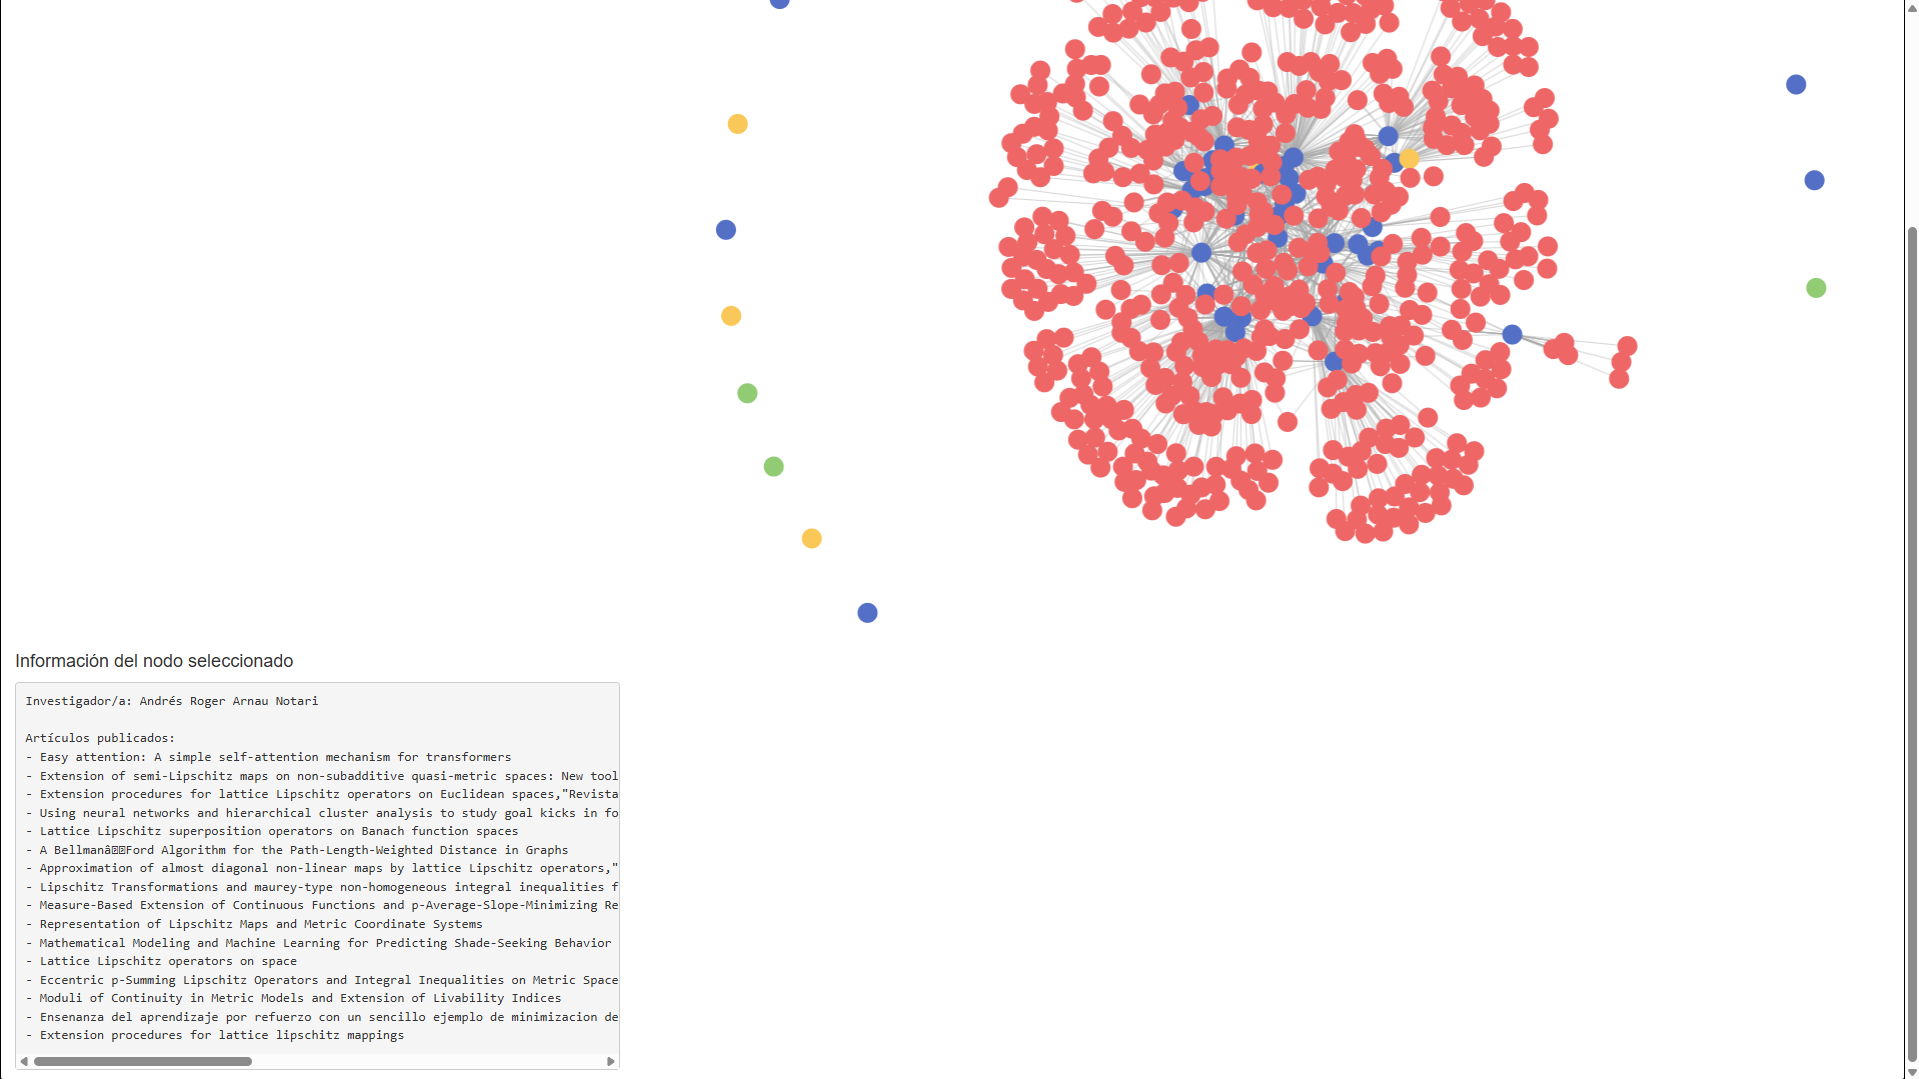
\includegraphics[width=\textwidth]{imgs/panel_investigador_revistas.png}
\end{minipage}
\hfill
\begin{minipage}{0.48\textwidth}
\centering
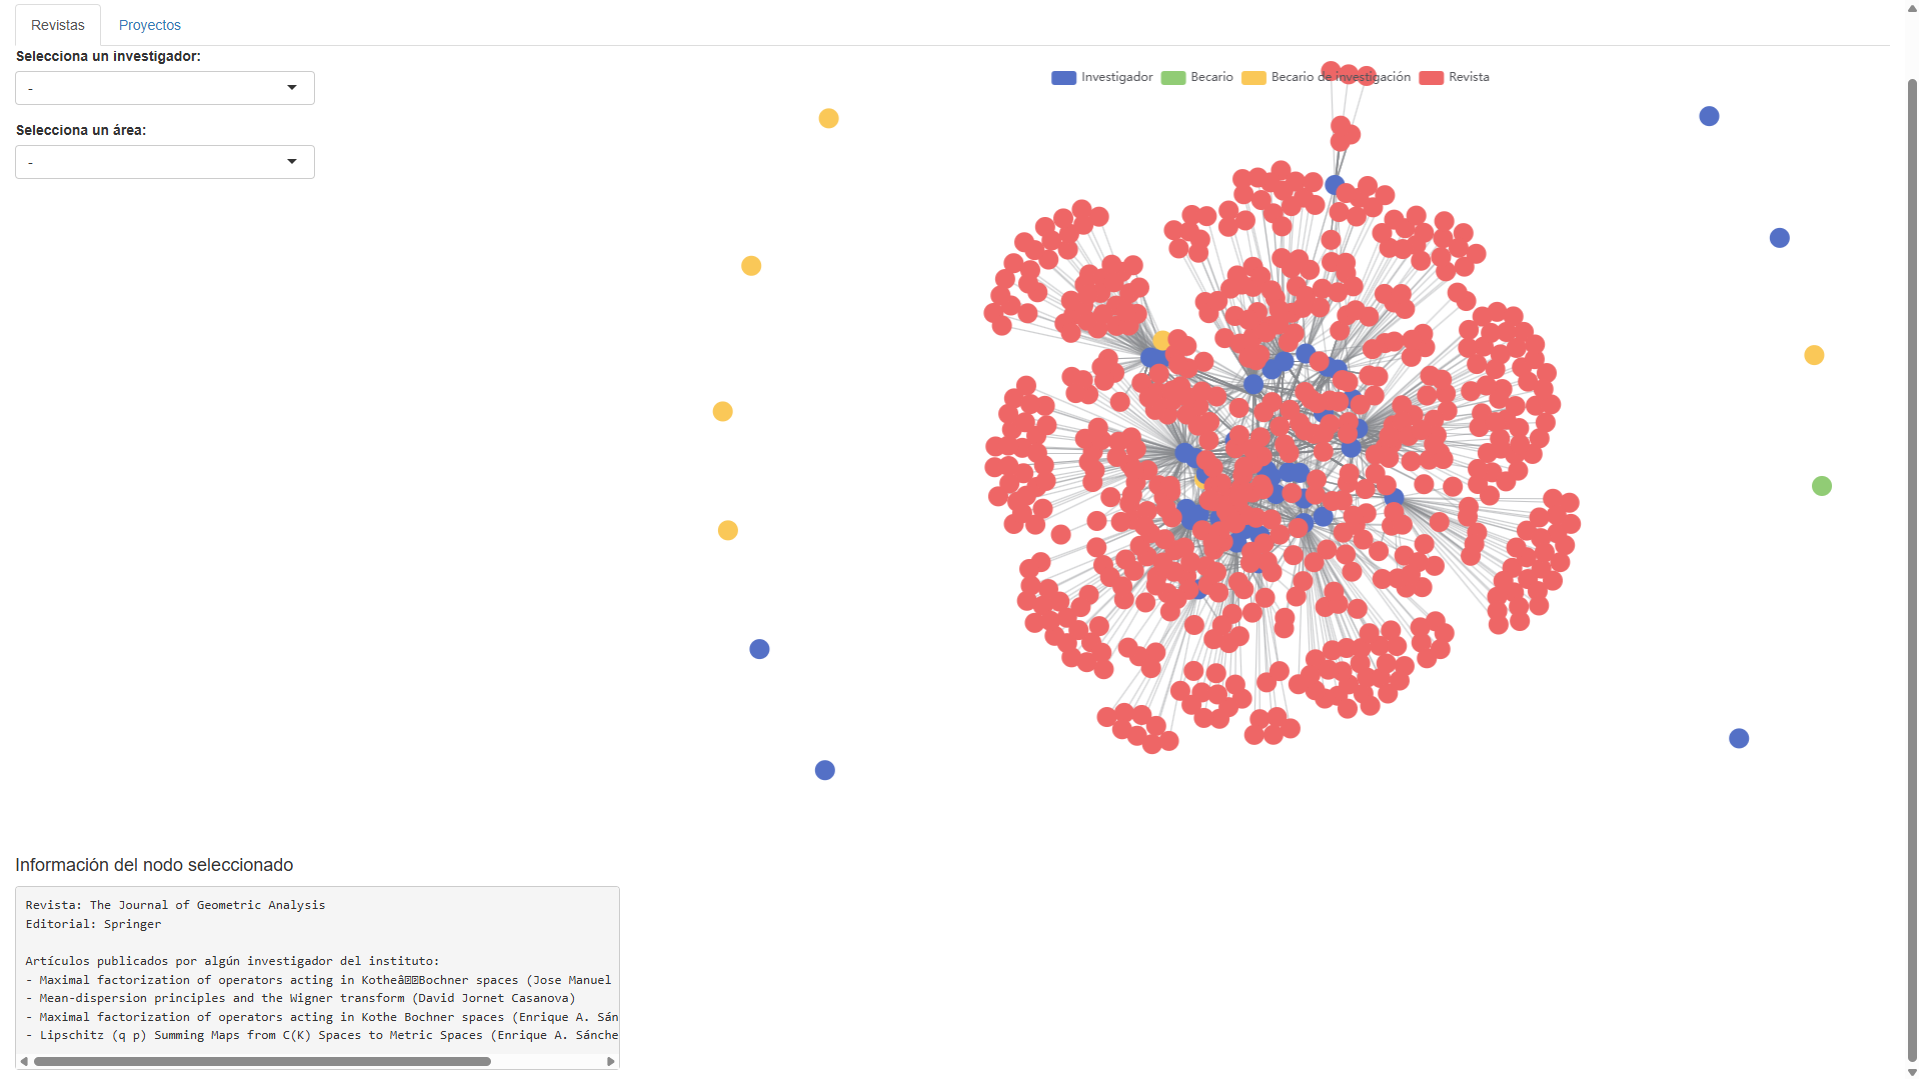
\includegraphics[width=\textwidth]{imgs/panel_revista.png}
\end{minipage}

\vspace{0.6em}

\begin{minipage}{0.48\textwidth}
\centering
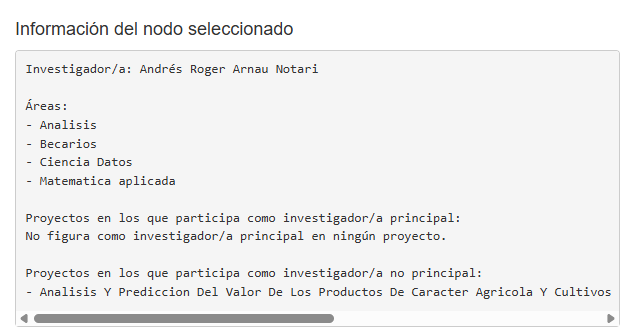
\includegraphics[width=\textwidth]{imgs/panel_investigador_proyectos.png}
\end{minipage}
\hfill
\begin{minipage}{0.48\textwidth}
\centering
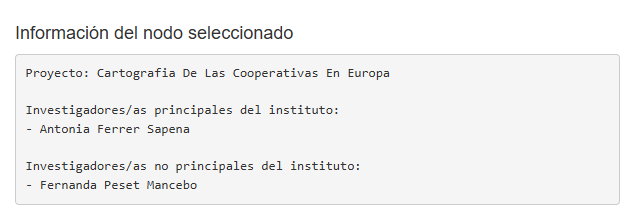
\includegraphics[width=\textwidth]{imgs/panel_proyecto.png}
\end{minipage}

\caption{Ejemplos de información mostrada al seleccionar distintos tipos de nodo en los grafos de producción académica.}
\label{fig:paneles_informativos}
\end{figure}

En conclusión, estos elementos permitían complementar la visualización global de los grafos con mecanismos de exploración más detallados. El usuario podía partir de una vista general de las relaciones y, posteriormente, aplicar filtros, ocultar categorías, consultar información emergente o seleccionar nodos concretos para acceder a los datos asociados.

\section{Valoración de la aplicación desarrollada}

La aplicación desarrollada permitió explotar la base de datos construida desde una perspectiva visual e interactiva. Su principal aportación fue transformar los ficheros tabulares en grafos explorables, facilitando la consulta de relaciones entre investigadores, revistas y proyectos, así como de las colaboraciones derivadas de publicaciones y proyectos compartidos. De este modo, la herramienta actuó como una capa de consulta sobre la base de datos, haciendo más accesible una información que en formato tabular resultaría menos inmediata.

La separación de la información en varias vistas resultó adecuada para evitar una única red excesivamente compleja. Los grafos de producción académica permitieron consultar relaciones entre investigadores y revistas o proyectos, mientras que los grafos de colaboración ofrecieron una perspectiva centrada en las relaciones entre miembros del instituto. Además, los elementos de interacción incorporados permitieron reducir la complejidad visual mediante filtros y acceder a información concreta mediante selección de nodos.

No obstante, la aplicación debe entenderse como una herramienta exploratoria condicionada por los datos disponibles. Algunos grafos pueden resultar densos en las vistas generales y la posición de los nodos debe interpretarse como un recurso visual, no como una medida analítica. Asimismo, la información mostrada depende de la completitud de las fuentes consultadas, por lo que la ausencia de una relación o registro no implica necesariamente su inexistencia. Aun así, la herramienta cumple su función principal dentro del proyecto, al facilitar la exploración visual de la actividad investigadora del IUMPA y servir como base para futuras ampliaciones.

%%%%%%%%%%%%%%%%%%%%%%%%%%%%%%%%%%%%%%%%%%%%%%%%%%%%%%%%%%%%%%%%%%%%%%%%%%%%%%%

%%%%%%%%%%%
%Capítulo 6
%%%%%%%%%%%

\chapter{Agrupación semántica de investigadores}

Tras la construcción de la base de datos y el desarrollo de los grafos interactivos, el proyecto ya permitía explorar la actividad investigadora del IUMPA desde una perspectiva relacional. Sobre esta base, se planteó estudiar si los datos recopilados podían revelar afinidades temáticas entre investigadores más allá de las colaboraciones y publicaciones observables. Para ello, se propuso una ampliación analítica basada en las revistas en las que publica cada investigador, partiendo de la idea de que dichas revistas pueden aportar información sobre sus áreas de interés al estar asociadas a diferentes campos.

A partir de esta hipótesis, se utilizaron palabras clave representativas de las revistas para construir perfiles temáticos de los investigadores y aplicar distintos métodos de agrupamiento orientados a identificar posibles grupos con intereses próximos.

El propósito de este análisis no fue obtener una clasificación cerrada de los miembros del instituto, sino explorar hasta qué punto la información disponible permitía detectar agrupaciones interpretables desde un punto de vista semántico. Por ello, el proceso combinó varias representaciones de los datos, distintos modelos de clustering y técnicas de reducción de dimensionalidad, valorando los resultados tanto mediante métricas cuantitativas como mediante su coherencia temática.

\section{Preparación del vocabulario temático}

Hasta este punto, las revistas habían servido principalmente para describir la actividad bibliográfica de los investigadores y construir relaciones dentro de la base de datos. En esta fase, esas mismas revistas comenzaron a tener la función adicional de actuar como indicadores temáticos. Para ello, se utilizaron las palabras clave asociadas a cada revista como forma de aproximar los campos con los que estaban relacionadas.

El objetivo no era describir cada revista exhaustivamente, sino disponer de un vocabulario suficientemente representativo para caracterizar su orientación temática. Esta decisión permitía trabajar con la revista como unidad intermedia entre el artículo individual y el investigador. De este modo, las palabras clave no se utilizaron para analizar el contenido detallado de cada publicación, sino para construir una aproximación general al tipo de temas presentes en los medios de publicación utilizados por los investigadores.

La obtención de este vocabulario combinó la consulta de fuentes especializadas sobre revistas con una fase de apoyo mediante herramientas de inteligencia artificial generativa. Este apoyo se utilizó únicamente para sugerir posibles términos temáticos cuando la información disponible era limitada o inexistente. Por tanto, las palabras generadas se trataron como propuestas iniciales y no como resultados definitivos, siendo revisadas posteriormente antes de incorporarse a las matrices de análisis.

Una vez recopiladas las palabras clave, fue necesario revisar el conjunto global de términos antes de utilizarlo en los modelos de agrupamiento. Algunas palabras aparecían asociadas a un gran número de revistas y, por tanto, aportaban poca capacidad diferenciadora. Otras, en cambio, eran demasiado específicas, lo que dificultaba la identificación de patrones compartidos entre investigadores. Por ello, la selección final buscó un equilibrio entre representatividad y utilidad para comparar perfiles temáticos.

Además de esta depuración, se revisó manualmente la coherencia del vocabulario para reducir duplicidades y unificar variantes muy próximas. Con ello se buscó que términos muy relacionados quedaran representados de forma consistente, evitando una fragmentación innecesaria del vocabulario. En consecuencia, las palabras clave no se emplearon como una recopilación directa de términos aislados, sino como un conjunto revisado y preparado para servir de base al análisis semántico.

Durante la revisión posterior de los primeros resultados se observó que no todos los términos del vocabulario contribuían del mismo modo a caracterizar intereses científicos. En particular, algunas palabras hacían referencia a localizaciones geográficas u otros elementos contextuales que podían aparecer vinculados a determinadas revistas, pero que no describían propiamente una línea de investigación. Aunque estos términos formaban parte de la información recopilada, su presencia podía desplazar la agrupación hacia coincidencias poco relevantes desde el punto de vista temático.

Por este motivo, se realizó una depuración adicional del vocabulario antes de consolidar la base final utilizada en el análisis. Esta revisión permitió eliminar términos que podían introducir ruido en la comparación entre investigadores y centrar la representación en palabras con mayor capacidad para describir ámbitos científicos. De esta forma, la selección final no solo buscó reducir términos poco informativos, sino también asegurar que el vocabulario empleado reflejara afinidades temáticas reales y no relaciones espurias derivadas de elementos accesorios.

Con este proceso quedó definida una base temática de revistas y palabras clave depuradas, preparada para trasladar posteriormente la información desde las revistas hacia los perfiles de los investigadores.

\section{Representación temática de los investigadores}

La base temática disponible relacionaba cada revista con un conjunto de palabras clave, pero el objetivo del análisis era comparar perfiles de investigadores. Por ello, el siguiente paso consistió en trasladar esa información desde las revistas hacia los investigadores, construyendo una representación en la que cada persona quedara descrita a partir de los términos asociados a las revistas en las que había publicado.

Para realizar esta transformación, se combinaron dos estructuras ya disponibles. La primera recogía la relación entre investigadores y revistas en las que habían publicado, mientras que la segunda asociaba cada revista con un conjunto de palabras clave. Al unir ambas estructuras, las palabras clave de cada revista pasaban a formar parte del perfil del investigador que había publicado en ella.

De este modo, no se asignaban palabras clave directamente a los investigadores, sino a través de las revistas que conectaban su actividad bibliográfica con determinados ámbitos temáticos. Esta decisión permitía conservar una trazabilidad clara entre los tres elementos implicados, es decir, investigador, revista y palabra clave. Así, además de saber qué términos caracterizaban a cada investigador, era posible identificar de qué revistas procedían, lo que facilitaba la interpretación posterior de los resultados.

A partir de esta información se construyó una primera matriz de representación basada en presencia y ausencia de términos. En esta matriz, cada fila correspondía a un investigador y cada columna a una palabra clave del vocabulario temático. El valor de cada celda indicaba si una determinada palabra estaba asociada o no al investigador correspondiente:

\[
M_{ij} =
\begin{cases}
1, & \text{si la palabra clave } j \text{ está asociada al investigador } i,\\
0, & \text{en caso contrario.}
\end{cases}
\]

Con esta estructura, la información textual quedaba transformada en un formato numérico sencillo, adecuado para calcular distancias entre perfiles y aplicar métodos de agrupamiento. Su interpretación también resultaba directa, ya que cada investigador quedaba descrito por el conjunto de términos asociados a las revistas en las que había publicado.

El proceso seguido para transformar las revistas publicadas en perfiles temáticos comparables se resume en la Figura~\ref{fig:flujo_representacion_tematica}.

\begin{figure}[H]
\centering
\small
\fbox{
\begin{minipage}{0.82\textwidth}
\centering
Revistas en las que ha publicado cada investigador

\vspace{0.2cm}
$\downarrow$

\vspace{0.2cm}
Palabras clave asociadas a esas revistas

\vspace{0.2cm}
$\downarrow$

\vspace{0.2cm}
Asignación de palabras clave al investigador

\vspace{0.2cm}
$\downarrow$

\vspace{0.2cm}
Perfil temático del investigador

\vspace{0.2cm}
$\downarrow$

\vspace{0.2cm}
Representación matricial de los perfiles

\vspace{0.2cm}
$\downarrow$

\vspace{0.2cm}
Entrada para los modelos de agrupamiento
\end{minipage}
}
\caption{Proceso de construcción de perfiles temáticos a partir de las revistas publicadas por los investigadores.}
\label{fig:flujo_representacion_tematica}
\end{figure}

La matriz binaria ofrecía una primera representación sencilla e interpretable de los perfiles temáticos. A partir de ella se realizaron distintas pruebas de agrupamiento, aplicando diferentes formas de comparar los perfiles de los investigadores. Sin embargo, los resultados obtenidos no mostraron una separación suficientemente clara entre grupos. Las métricas de evaluación, con valores bajos del índice de Silhouette en las mejores pruebas iniciales, indicaban que las agrupaciones generadas no eran lo bastante consistentes. Por ello, se decidió no forzar una interpretación de estos primeros resultados y revisar la forma en que estaban representados los perfiles temáticos.

El principal problema de este enfoque era que la similitud entre investigadores dependía de coincidencias literales entre términos. Por ello, dos perfiles próximos desde un punto de vista conceptual podían aparecer como poco similares si las revistas asociadas a cada uno estaban descritas mediante vocabularios distintos. Esta situación resultaba especialmente relevante en un contexto como el del IUMPA, donde pueden existir líneas de trabajo cercanas expresadas con términos parcialmente diferentes.

Para tratar de mejorar esta situación, y antes de pasar al enfoque semántico, se introdujo una ponderación sobre la matriz inicial. El objetivo era evitar que todas las palabras clave tuvieran el mismo peso dentro de la comparación entre investigadores. En particular, se buscaba reducir la influencia de términos excesivamente comunes, que podían aparecer en muchos perfiles y aportar poca capacidad diferenciadora, así como de palabras demasiado raras, cuya aparición aislada podía condicionar de forma desproporcionada los resultados.

La ponderación aplicada consistió en una adaptación propia basada en una penalización simétrica con forma gaussiana. Esta decisión toma como referencia la ponderación de términos en representaciones vectoriales de texto~\cite{salton} y el uso de funciones gaussianas para asignar pesos decrecientes conforme un valor se aleja de un centro~\cite{gaussian_function}. En este caso no se utiliza el factor de normalización de la distribución normal, ya que no se pretende definir una densidad de probabilidad, sino asignar un peso relativo a cada palabra clave según la distancia de su frecuencia respecto a la media del vocabulario.

Con este enfoque, las palabras con frecuencias intermedias recibían mayor peso, al considerarse potencialmente más representativas para comparar perfiles, mientras que los términos demasiado frecuentes o demasiado aislados quedaban penalizados. El peso de una palabra clave \(j\) se definió como:

\[
w_j = e^{-\frac{(f_j - \mu)^2}{2\sigma^2}}
\]

donde \(f_j\) representa la frecuencia de la palabra clave \(j\), \(\mu\) la frecuencia media de las palabras clave y \(\sigma\) un parámetro que controla el grado de penalización aplicado a los términos situados en los extremos de la distribución de frecuencias.

La estrategia permitió incorporar una primera forma de discriminación dentro de la representación. No obstante, aunque la ponderación mejoraba conceptualmente la matriz binaria, los resultados siguieron sin ofrecer una separación numéricamente satisfactoria entre grupos. La comparación continuaba dependiendo de la presencia explícita de los términos en el vocabulario, por lo que no resolvía la limitación principal del enfoque basado en coincidencias literales.

A partir de esta evaluación, se decidió pasar a una representación más flexible mediante \textit{word embeddings}. En lugar de tratar cada palabra clave como una etiqueta independiente, este enfoque representa los términos mediante vectores numéricos situados en un espacio semántico. En este caso se utilizó la librería \textit{sentence-transformers}, basada en el enfoque Sentence-BERT~\cite{sentencebert}, junto con el modelo multilingüe \textit{paraphrase-multilingual-MiniLM-L12-v2}, que transforma cada término en un vector denso de 384 dimensiones~\cite{minilm_multilingual}. De este modo, dos palabras distintas pueden aparecer próximas en dicho espacio si están relacionadas conceptualmente, aunque no coincidan de forma literal.

Esta propiedad resultaba útil para el objetivo del análisis, ya que permitía comparar perfiles de investigadores no solo a partir de las palabras exactas que compartían, sino también considerando la relación conceptual entre los términos que caracterizaban sus revistas. Así, la representación dejaba de depender exclusivamente de coincidencias textuales y pasaba a incorporar una noción de proximidad conceptual entre palabras clave.

Para construir el perfil semántico de cada investigador, se obtuvieron los vectores correspondientes a sus palabras clave y se calculó una representación agregada a partir de ellos. Formalmente, si \(K_i\) representa el conjunto de palabras clave asociadas al investigador \(i\), y \(\mathbf{e}(w)\) representa el vector semántico de una palabra \(w\), el perfil del investigador puede expresarse como:

\[
\mathbf{v}_i = \frac{1}{|K_i|}\sum_{w \in K_i} \mathbf{e}(w)
\]

De esta forma, cada investigador dejó de estar representado únicamente por una lista de términos o por una fila de una matriz binaria, y pasó a estar descrito mediante un vector continuo que resumía, de forma aproximada, el contenido semántico de su perfil temático.

Esta transformación permitió trabajar con una representación más flexible de los investigadores. Mientras que la matriz binaria resultaba útil como primera aproximación interpretable, los embeddings incorporaban una dimensión semántica que permitía comparar perfiles más allá de la coincidencia exacta de palabras clave, recogiendo afinidades entre términos conceptualmente próximos.

\section{Clustering y evaluación}

Una vez que cada investigador quedó descrito mediante un perfil temático, el análisis podía avanzar desde la representación individual hacia la búsqueda de patrones compartidos. La cuestión, por tanto, se convirtió en estudiar si esos perfiles permitían reconocer grupos con intereses próximos, no definidos únicamente por las áreas institucionales del IUMPA.

Este planteamiento se abordó como una tarea de aprendizaje no supervisado, ya que no se buscaba entrenar un modelo para reproducir una clasificación conocida, sino explorar la estructura interna de los perfiles construidos a partir de revistas y palabras clave.

Aunque el instituto cuenta con áreas de trabajo asignadas a los investigadores, estas no se mantuvieron como variable de entrada en el modelo de clustering. En las pruebas realizadas, su inclusión hacía que la agrupación quedara fuertemente condicionada por dicha clasificación previa, reuniendo a los investigadores principalmente según el área a la que pertenecían. Por este motivo, se decidió excluirlas del análisis y trabajar únicamente con la información derivada de las revistas y del vocabulario temático, permitiendo al agrupamiento explorar posibles afinidades complementarias a las áreas institucionales, en lugar de limitarse a reproducirlas.

El proceso de agrupamiento se desarrolló de forma experimental, comparando distintas configuraciones a partir de las representaciones descritas previamente. Esta fase no consistió en aplicar un único modelo, sino en probar varias formas de representar los perfiles, medir la proximidad entre ellos y construir agrupaciones. Para ello se trabajó de manera progresiva, comenzando con representaciones basadas en palabras clave explícitas y avanzando posteriormente hacia representaciones semánticas mediante \textit{word embeddings}.

Cada configuración del proceso dependía, por tanto, de la representación de entrada, la versión del vocabulario, la medida de proximidad, el método de agrupamiento, el número de grupos considerado y la posible aplicación de reducción de dimensionalidad. La Tabla~\ref{tab:elementos_clustering} resume los componentes principales considerados durante esta fase experimental.

\begin{table}[H]
\centering
\small
\renewcommand{\arraystretch}{1.05}
\begin{tabular}{
>{\centering\arraybackslash}m{0.24\textwidth}
m{0.36\textwidth}
m{0.30\textwidth}
}
\hline
\textbf{Elemento} & \textbf{Opciones consideradas} & \textbf{Función dentro del análisis} \\
\hline
Representación de entrada & Matriz binaria, matriz ponderada y embeddings semánticos & Definir cómo se describe temáticamente cada investigador \\
\hline
Versión del vocabulario & Vocabulario completo y vocabulario depurado sin términos de localización & Comprobar si las agrupaciones respondían a afinidades temáticas o a factores contextuales \\
\hline
Medidas de proximidad & Jaccard, Hamming, coseno, correlación, euclídea y Manhattan & Cuantificar la cercanía o diferencia entre perfiles de investigadores \\
\hline
Métodos de agrupamiento & Clustering jerárquico, K-means, PAM, Fuzzy C-Means, Spectral Clustering, GMM, DBSCAN y HDBSCAN & Comparar distintas formas de construir grupos a partir de los perfiles \\
\hline
Número de grupos o parámetros de agrupamiento & Distintos valores de \(k\) en k-means, cortes del dendrograma en jerárquico y variación de parámetros como \(\varepsilon\) en DBSCAN & Estudiar cómo cambia la estructura de grupos según la configuración del modelo \\
\hline
Reducción de dimensionalidad & Configuraciones sin reducción, PCA y UMAP & Comparar los agrupamientos obtenidos en el espacio original y en proyecciones de menor dimensión \\
\hline
Evaluación & Índice de Silhouette, visualizaciones, revisión manual de la coherencia temática y comparación de solapamientos & Comparar configuraciones y valorar la coherencia de las agrupaciones \\
\hline
\end{tabular}
\caption{Elementos considerados en el proceso de agrupamiento temático.}
\label{tab:elementos_clustering}
\end{table}

\subsection{Primeras pruebas con palabras clave explícitas}

La primera aproximación al agrupamiento se realizó utilizando directamente la matriz de presencia y ausencia de palabras clave. En esta representación, cada investigador quedaba descrito por los términos asociados a las revistas en las que había publicado, sin incorporar todavía ponderaciones ni relaciones semánticas entre palabras. El objetivo de esta fase era comprobar si las coincidencias literales entre palabras clave bastaban para identificar grupos de investigadores con perfiles temáticos próximos.

Sobre esta matriz se probaron distintas medidas de proximidad. En primer lugar, se utilizaron medidas especialmente adecuadas para datos binarios, como Jaccard y Hamming, ya que permiten comparar perfiles según la coincidencia o diferencia en la presencia de términos. Además, también se probaron otras medidas como coseno, correlación, distancia euclídea y Manhattan, con el fin de observar si la estructura de los grupos variaba al cambiar la forma de medir la proximidad entre investigadores.

En cuanto a los métodos de clusterización, la variante jerárquica fue una de las primeras alternativas utilizadas en esta fase, ya que permitía analizar diferentes particiones a partir de un mismo árbol de agrupamiento. Para ello, se ensayaron distintos criterios de enlace, como \textit{average}, \textit{complete}, \textit{single} y \textit{ward.D2}, y se compararon varios valores de \(k\). Esta variedad de configuraciones permitía comprobar si los grupos aparecían de forma estable o si dependían en exceso de la métrica y del enlace utilizados.

Junto a las pruebas jerárquicas, también se aplicaron otros métodos de agrupamiento sobre la misma representación, como K-means, PAM, Fuzzy C-Means, Spectral Clustering o GMM. La finalidad de estas pruebas era comprobar si las limitaciones observadas procedían del algoritmo de clustering o de la propia representación basada en coincidencias literales de palabras clave. La Tabla~\ref{tab:primeras_pruebas_keywords} muestra un resumen de las principales configuraciones probadas en esta fase inicial y de la interpretación general obtenida a partir de ellas.

\begin{table}[H]
\centering
\small
\renewcommand{\arraystretch}{1.25}
\begin{tabular}{
>{\centering\arraybackslash}m{0.30\textwidth}
>{\centering\arraybackslash}m{0.18\textwidth}
m{0.42\textwidth}
}
\hline
\textbf{Configuración} & \textbf{Mejor Silhouette} & \textbf{Observación principal} \\
\hline
Jerárquico + Jaccard & 0.252 & Solapamiento entre grupos y separación limitada \\
\hline
Jerárquico + Euclídea & 0.210 & División general en pocos grupos, con baja cohesión interna \\
\hline
Jerárquico + Coseno & 0.273 & Algunas particiones razonables, pero sin estructura suficientemente clara \\
\hline
Jerárquico + Correlación & 0.258 & Resultados moderados, con dependencia de la partición elegida \\
\hline
Jerárquico + Manhattan & 0.329 & Mejor comportamiento relativo en esta fase, aunque todavía con interpretación limitada \\
\hline
K-means + Euclídea & 0.129 & Particiones poco interpretables sin mejora frente al enfoque jerárquico \\
\hline
K-means + Euclídea + PCA & 0.198 & Ligera mejora respecto a K-means, pero todavía insuficiente \\
\hline
PAM + Jaccard & 0.174 & No ofreció una estructura clara de grupos \\
\hline
PAM + Manhattan & 0.220 & Resultado algo mejor que Jaccard, pero sin una separación suficientemente sólida \\
\hline
Fuzzy C-Means & 0.161 & Agrupaciones débiles y poco útiles para la interpretación temática \\
\hline
Spectral Clustering & 0.098 & Resultado muy bajo, sin estructura aprovechable \\
\hline
GMM & -0.066 & Resultado negativo, indicando asignaciones no adecuadas \\
\hline
\end{tabular}
\caption{Resumen de las primeras pruebas realizadas con palabras clave explícitas.}
\label{tab:primeras_pruebas_keywords}
\end{table}

Los resultados obtenidos en esta primera fase mostraron una separación limitada entre grupos. La mejor configuración dentro del clustering jerárquico fue la basada en distancia Manhattan, con un valor máximo de Silhouette de 0.329, mientras que el resto de métricas se mantuvieron en valores más bajos. Los métodos alternativos (K-means, PAM, Fuzzy C-Means, Spectral Clustering y GMM) tampoco ofrecieron una mejora clara, produciendo valores reducidos y agrupaciones difíciles de interpretar en general.

Para representar gráficamente estas primeras pruebas se empleó una proyección MDS (\textit{Multidimensional Scaling}), una técnica que permite visualizar en dos dimensiones las distancias calculadas entre perfiles. De este modo, resulta posible observar si los grupos aparecen separados o si, por el contrario, existe solapamiento entre ellos.

Además de los valores numéricos, las visualizaciones generadas durante esta fase permitieron observar solapamientos entre perfiles y particiones poco equilibradas. La Figura~\ref{fig:primeras_pruebas_keywords} muestra una configuración representativa de esta primera etapa, basada en distancia Manhattan y clustering jerárquico con enlace \textit{average}. Su objetivo no es presentar un modelo final, sino ilustrar las limitaciones observadas al trabajar únicamente con coincidencias explícitas de palabras clave. Aunque esta configuración fue la que obtuvo el mejor valor de Silhouette dentro de las pruebas iniciales, la proyección MDS muestra una separación todavía difusa entre perfiles y el gráfico de Silhouette refleja diferencias claras en la cohesión de los grupos obtenidos.

\begin{figure}[H]
\centering
\begin{minipage}{0.48\textwidth}
\centering
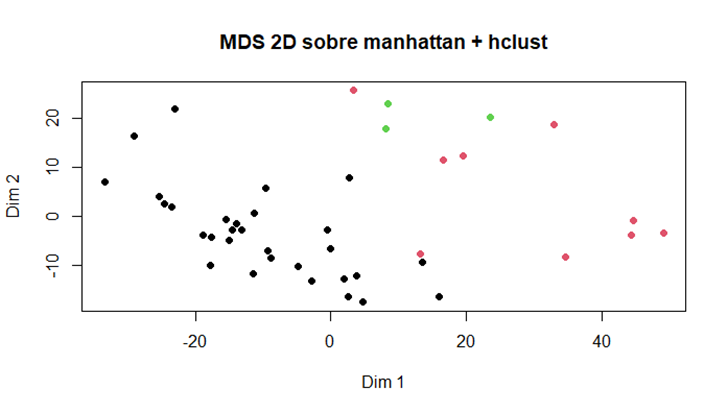
\includegraphics[width=\textwidth]{imgs/mds_keywords_manhattan.png}
\caption*{(a) Proyección MDS}
\end{minipage}
\hfill
\begin{minipage}{0.48\textwidth}
\centering
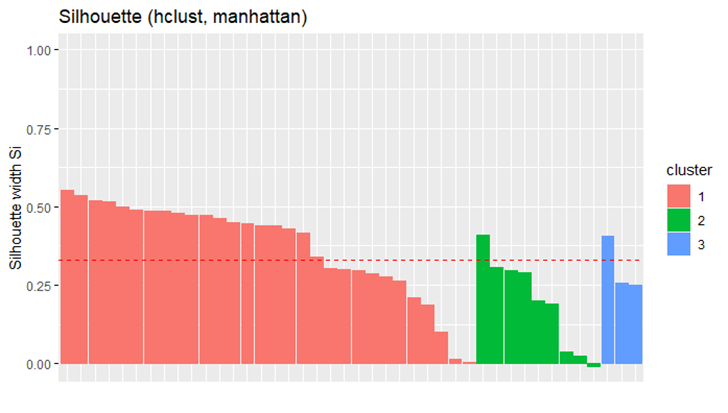
\includegraphics[width=\textwidth]{imgs/silhouette_keywords_manhattan.png}
\caption*{(b) Gráfico de Silhouette}
\end{minipage}
\caption{Visualización representativa de una de las primeras pruebas basadas en palabras clave explícitas.}
\label{fig:primeras_pruebas_keywords}
\end{figure}

La lectura conjunta de la tabla y de las visualizaciones muestra que estas primeras agrupaciones no ofrecían una separación suficientemente clara. En algunas configuraciones aparecían grupos parcialmente diferenciados, pero la estructura general seguía siendo débil y cambiaba de forma apreciable según la distancia, el método o el número de grupos elegido. Esto sugería que el problema no estaba únicamente en el algoritmo de clustering, sino también en la forma en que se estaban representando los perfiles.

La matriz binaria permitió comprobar una primera idea, pero también mostró que la comparación entre investigadores seguía siendo demasiado simple. Todos los términos tenían el mismo peso, independientemente de si eran muy frecuentes, muy específicos o realmente útiles para diferenciar perfiles. Por ello, antes de abandonar el enfoque basado en palabras clave explícitas, se planteó una representación intermedia en la que el vocabulario estuviera ponderado, con el objetivo de mejorar los resultados sin renunciar del todo a la simplicidad de la representación. Con esta modificación, la comparación entre investigadores podía depender menos de términos poco informativos y reflejar mejor las diferencias temáticas entre perfiles.

\subsection{Ponderación gaussiana del vocabulario}

Tras las primeras pruebas con la matriz binaria, se introdujo una segunda representación basada en la ponderación del vocabulario. La idea era mantener una estructura sencilla e interpretable, todavía basada en palabras clave explícitas, pero evitando que todos los términos tuvieran la misma importancia dentro de la comparación entre investigadores.

La matriz ponderada mantenía la misma organización que la matriz inicial, con investigadores en las filas y palabras clave en las columnas. Sin embargo, los valores dejaban de indicar únicamente presencia o ausencia, ya que cada palabra incorporaba un peso dependiente de su frecuencia. De este modo, la presencia de una palabra no contribuía siempre de la misma forma, sino según el peso asignado a dicha palabra.

La ponderación aplicada se basó en una penalización simétrica con forma gaussiana. Con este enfoque, las palabras con frecuencias intermedias recibían mayor peso, al considerarse potencialmente más útiles para diferenciar perfiles, mientras que los términos demasiado frecuentes y demasiado aislados quedaban penalizados por aportar poca capacidad discriminativa.

Sobre esta representación ponderada se repitieron varias de las pruebas realizadas en la fase anterior y se incorporaron algunos ajustes específicos. En concreto, se volvieron a comparar distintas medidas de proximidad, como coseno, Jaccard, correlación, distancia euclídea y Manhattan, y se aplicaron métodos de agrupamiento como clustering jerárquico, K-means y PAM. Además, se probaron distintos valores del parámetro \(\sigma\), con el objetivo de observar cómo variaba el efecto de la ponderación al penalizar con mayor o menor intensidad las frecuencias alejadas de la media.

La Tabla~\ref{tab:pruebas_matriz_ponderada} resume algunas de las configuraciones más representativas de esta fase, no con el objetivo de recoger todas las combinaciones posibles, sino de mostrar que la ponderación no tuvo un efecto uniforme sobre todos los modelos, ya que en algunas configuraciones mejoró los valores de Silhouette, mientras que en otras apenas aportó mejora o incluso produjo agrupaciones poco útiles desde el punto de vista interpretativo.

\begin{table}[H]
\centering
\small
\renewcommand{\arraystretch}{1.25}
\begin{tabular}{
>{\centering\arraybackslash}m{0.34\textwidth}
>{\centering\arraybackslash}m{0.18\textwidth}
m{0.38\textwidth}
}
\hline
\textbf{Configuración} & \textbf{Mejor Silhouette} & \textbf{Observación principal} \\
\hline
Coseno + Jerárquico & 0.169 & No mejoró de forma clara la separación entre grupos \\
\hline
Jaccard + Jerárquico & 0.123 & Resultados bajos y poca estructura interpretable \\
\hline
Correlación + Jerárquico & 0.178 & Mejora limitada, sin agrupaciones suficientemente sólidas \\
\hline
Manhattan + Jerárquico, \(\sigma=1\) & 0.351 & Mejor comportamiento que la matriz binaria, aunque todavía con interpretación limitada \\
\hline
Manhattan + Jerárquico, \(\sigma=0.5\) & 0.445 & Mejor resultado numérico, pero con aparición de un grupo dominante \\
\hline
Euclídea + Jerárquico & 0.198 & Separación limitada entre perfiles \\
\hline
K-means + Euclídea & 0.304 & Mejora respecto a K-means inicial, pero con clusters poco representativos \\
\hline
PAM + Jaccard & 0.120 & No aportó una mejora clara frente a otras configuraciones \\
\hline
\end{tabular}
\caption{Resumen de pruebas realizadas con la matriz ponderada de palabras clave.}
\label{tab:pruebas_matriz_ponderada}
\end{table}

Los resultados muestran que la ponderación no produjo una mejora homogénea en todas las configuraciones. Algunas medidas, como coseno, Jaccard o correlación, siguieron ofreciendo valores bajos, mientras que la distancia Manhattan fue la que mostró el mejor comportamiento relativo. Con \(\sigma=1\), esta configuración alcanzó un valor máximo de Silhouette de 0.351, ligeramente superior al obtenido con la matriz binaria. Al reducir \(\sigma\), el valor aumentó hasta 0.445, pero este incremento debía interpretarse con cautela.

El principal problema apareció precisamente en las configuraciones con mejores valores numéricos. Al aplicar una penalización más intensa, el modelo tendía a concentrar a una parte importante de los investigadores en un grupo dominante, dejando el resto en grupos de menor tamaño con perfiles más extremos. Esta estructura elevaba el valor medio de Silhouette, pero no necesariamente producía una agrupación más útil desde el punto de vista temático. Por tanto, la mejora de la métrica no podía interpretarse automáticamente como una mejora real del clustering.

La Figura~\ref{fig:ponderada_manhattan_sigma05} muestra una configuración representativa de esta fase, basada en distancia Manhattan, clustering jerárquico con enlace \textit{average} y \(\sigma=0.5\). Su interés no está en presentar una solución final, sino en ilustrar la diferencia entre mejora numérica y utilidad interpretativa.

\begin{figure}[H]
\centering
\begin{minipage}{0.48\textwidth}
\centering
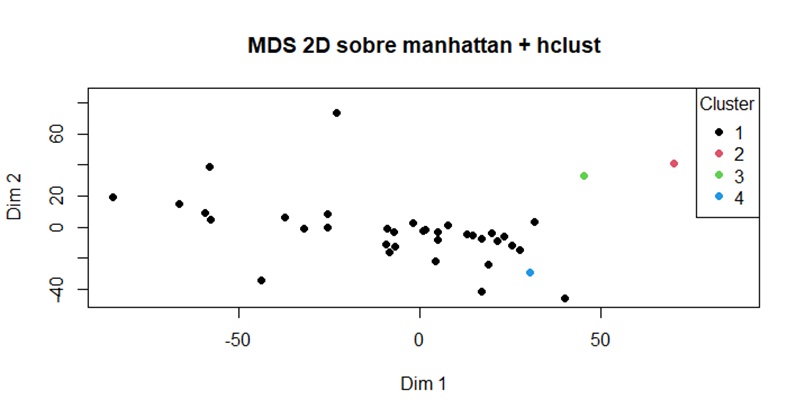
\includegraphics[width=\textwidth]{imgs/mds_ponderada_manhattan_sigma05.png}
\caption*{(a) Proyección MDS}
\end{minipage}
\hfill
\begin{minipage}{0.48\textwidth}
\centering
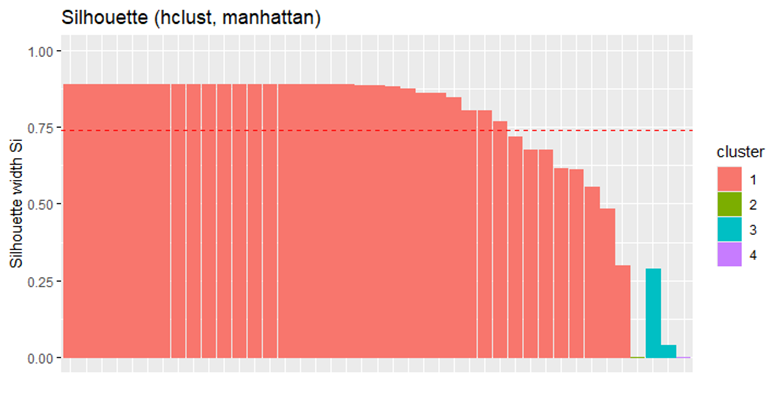
\includegraphics[width=\textwidth]{imgs/silhouette_ponderada_manhattan_sigma05.png}
\caption*{(b) Gráfico de Silhouette}
\end{minipage}
\caption{Visualización representativa de una prueba con matriz ponderada.}
\label{fig:ponderada_manhattan_sigma05}
\end{figure}

En esta configuración se obtenía un valor de Silhouette superior al de las pruebas iniciales con matriz binaria, pero la estructura resultante no muestra una distribución equilibrada de los perfiles. La agrupación queda dominada por un grupo principal que reúne a la mayor parte de los investigadores, mientras que el resto de grupos quedan formados por pocos perfiles más extremos. Por tanto, la mejora numérica no garantiza una interpretación temática más clara ni una partición más útil para el objetivo del análisis.

En resumen, esta fase permitió comprobar que la ponderación gaussiana refinaba la matriz inicial, pero no resolvía la limitación principal del enfoque. Los términos ya no contribuían todos por igual, pero la comparación entre investigadores seguía dependiendo de la presencia explícita de palabras clave compartidas. Por ello, el análisis avanzó hacia una representación semántica mediante \textit{word embeddings}, capaz de comparar perfiles a partir de la proximidad conceptual entre términos distintos.

\subsection{Representaciones semánticas, métodos de agrupamiento y reducción de dimensionalidad}

Tras las pruebas con la matriz binaria y con la matriz ponderada, el análisis se trasladó a las representaciones semánticas mediante \textit{word embeddings}. Esta decisión se tomó porque, en las fases anteriores, la comparación entre investigadores seguía dependiendo de la coincidencia explícita entre palabras clave. Con los embeddings, cada investigador quedaba descrito mediante un vector continuo que resumía el contenido semántico de sus términos, lo que permitía comparar perfiles no solo por las palabras exactas que compartían, sino también por la proximidad conceptual entre ellas.

Sobre esta nueva representación se abrió una fase más amplia de pruebas. Ya no se trataba únicamente de comparar matrices de palabras clave, sino de estudiar cómo se comportaban los perfiles semánticos bajo distintas medidas de proximidad, métodos de agrupamiento y técnicas de reducción de dimensionalidad. En esta etapa se probaron medidas como coseno, correlación, distancia euclídea y Manhattan, con el objetivo de comprobar si la estructura de grupos dependía de una única forma de medir la cercanía entre perfiles o si aparecían patrones similares bajo distintas métricas.

El clustering jerárquico fue una de las alternativas principales en esta fase. Se utilizó una estrategia aglomerativa, principalmente con enlace promedio (\textit{average}), que permitía construir progresivamente un árbol de agrupamiento y estudiar distintos cortes del dendrograma. Esta característica resultaba adecuada para el carácter exploratorio del análisis, ya que no obligaba a fijar un único número de grupos desde el inicio. En las pruebas realizadas se compararon distintos valores de \(k\), de forma que era posible observar cómo cambiaban las particiones al variar el nivel de corte del árbol.

Las primeras configuraciones jerárquicas sobre embeddings ofrecieron valores de Silhouette superiores a los obtenidos en varias pruebas con palabras clave explícitas. Por ejemplo, las pruebas con distancia Manhattan, correlación o coseno alcanzaron valores en torno a 0.4 en algunas configuraciones. Sin embargo, estos resultados también debían interpretarse con cautela, ya que varias particiones seguían mostrando una estructura dominada por un grupo principal de gran tamaño. Por tanto, aunque la representación semántica mejoraba la capacidad de comparación entre términos, la calidad numérica de una configuración no garantizaba por sí sola una agrupación equilibrada ni directamente interpretable.

Además del clustering jerárquico, se probaron métodos basados en densidad, concretamente DBSCAN~\cite{dbscan} y HDBSCAN~\cite{hdbscan}. Estos métodos resultaban interesantes porque no parten necesariamente de un número fijo de grupos, sino que intentan identificar regiones densas de puntos y separar observaciones que no encajan claramente en ningún grupo. En el caso de DBSCAN se probaron distintos valores del parámetro \(\varepsilon\), comparando configuraciones con y sin reducción de dimensionalidad previa mediante PCA. No obstante, estas pruebas tendieron a generar un único grupo principal junto con un porcentaje elevado de observaciones tratadas como ruido, por lo que no ofrecieron una partición suficientemente útil para el objetivo interpretativo del análisis.

HDBSCAN se probó en la misma línea, como una alternativa más flexible para trabajar con estructuras de densidad variable. Su inclusión respondía al interés por comprobar si los perfiles formaban regiones densas sin necesidad de fijar previamente un número de grupos. Sin embargo, las pruebas realizadas tampoco proporcionaron una estructura suficientemente clara para orientar el análisis final. Por ello, los métodos basados en densidad se mantuvieron como una vía exploratoria, mientras que el análisis posterior se centró principalmente en configuraciones jerárquicas, que permitían estudiar de forma más controlada el efecto de la métrica de distancia, el número de grupos y la reducción dimensional.

También se valoraron técnicas orientadas a representar la estructura global de los perfiles en un espacio de menor dimensión. Entre ellas se consideró PCA~\cite{jolliffe}, utilizada como reducción lineal para conservar una proporción elevada de la varianza antes de aplicar determinados métodos de clustering. Esta opción permitía comprobar si una representación más compacta de los embeddings facilitaba la formación de grupos o reducía parte del ruido presente en el espacio original. En algunas pruebas, la combinación de PCA con clustering jerárquico incrementó el valor de Silhouette, aunque volvió a aparecer el problema de grupos dominantes, por lo que tampoco podía considerarse una solución suficiente por sí misma.

Dentro de las técnicas de reducción no lineal, UMAP adquirió un papel especialmente relevante~\cite{umap}. A diferencia de PCA, que proyecta los datos mediante combinaciones lineales, UMAP busca preservar relaciones de vecindad entre observaciones en un espacio de menor dimensión, lo que lo hacía adecuado para trabajar con embeddings semánticos, ya que permitía comprobar si los perfiles de investigadores presentaban una estructura más clara al proyectarse en dos dimensiones.

En las pruebas iniciales con UMAP, su combinación con clustering jerárquico basado en distancia coseno produjo una separación más clara que otras configuraciones. En concreto, se obtuvo un valor medio de Silhouette de 0.602 y se identificaron tres grupos principales, lo que suponía una mejora respecto a las pruebas jerárquicas realizadas directamente sobre los embeddings, como Manhattan con \(S=0.413\), Manhattan con PCA con \(S=0.445\), o correlación/coseno con \(S=0.409\). Este resultado indicaba que la reducción no lineal podía facilitar la aparición de estructuras más diferenciadas en el espacio semántico y justificaba revisar con más detalle este tipo de configuración en las fases posteriores del análisis.

La Tabla~\ref{tab:pruebas_embeddings_iniciales} recoge una selección de las configuraciones más representativas probadas sobre los perfiles semánticos iniciales. No se pretende recoger todas las combinaciones exploradas, sino resumir los comportamientos principales observados al aplicar distintas medidas de proximidad, métodos de agrupamiento y técnicas de reducción de dimensionalidad sobre los embeddings.

\begin{table}[H]
\centering
\small
\renewcommand{\arraystretch}{1.25}
\begin{tabular}{
>{\centering\arraybackslash}m{0.34\textwidth}
>{\centering\arraybackslash}m{0.18\textwidth}
m{0.38\textwidth}
}
\hline
\textbf{Configuración} & \textbf{Resultado} & \textbf{Observación principal} \\
\hline
Manhattan + Jerárquico & \(S=0.413\) & Buen valor numérico, pero con aparición de un grupo dominante \\
\hline
Manhattan + PCA + Jerárquico & \(S=0.445\) & Mejora numérica, aunque mantiene el problema de grupo dominante \\
\hline
Correlación + Jerárquico & \(S=0.409\) & Resultado alto, pero con estructura dominada por un grupo principal \\
\hline
Coseno + Jerárquico & \(S=0.409\) & Comportamiento similar al de correlación, sin resolver la interpretación de grupos \\
\hline
Coseno + DBSCAN & 2 clusters y 45.2\% de ruido & Incluso con PCA y \(\varepsilon=0.45\), mantiene mucho ruido \\
\hline
Coseno + UMAP + Jerárquico & \(S=0.602\) & Separación inicial más clara, pendiente de revisión posterior \\
\hline
\end{tabular}
\caption{Resumen de pruebas iniciales realizadas sobre representaciones semánticas mediante embeddings.}
\label{tab:pruebas_embeddings_iniciales}
\end{table}

En el caso de DBSCAN y HDBSCAN no se recoge un valor de Silhouette comparable al resto de configuraciones, ya que estas pruebas no generaron una partición estable con varios grupos útiles para la evaluación. En particular, DBSCAN tendía a producir un único grupo principal junto con un porcentaje elevado de observaciones clasificadas como ruido, mientras que HDBSCAN tampoco ofreció una estructura suficientemente clara.

En líneas generales, los resultados muestran que las representaciones semánticas aumentaban el potencial de separación respecto a las matrices basadas en coincidencias literales, aunque la calidad de los grupos seguía dependiendo de la configuración utilizada. Algunas combinaciones alcanzaban valores de Silhouette superiores a los enfoques anteriores, pero todavía generaban particiones poco equilibradas, mientras que los métodos basados en densidad no ofrecían una estructura suficientemente clara. En este contexto, la combinación de UMAP, distancia coseno y clustering jerárquico apareció como la alternativa más prometedora dentro de esta fase inicial.

La Figura~\ref{fig:umap_embeddings_inicial} muestra la proyección UMAP obtenida en esta fase inicial con embeddings. Esta visualización permite observar por qué esta configuración resultó prometedora, ya que los perfiles aparecen organizados en tres grupos principales con una separación más clara que en las representaciones anteriores.

\begin{figure}[H]
\centering
\begin{minipage}{0.48\textwidth}
\centering
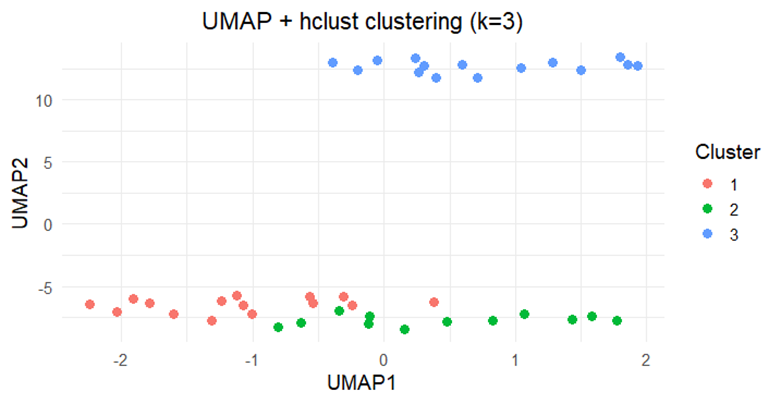
\includegraphics[width=\textwidth]{imgs/umap_embeddings_inicial.png}
\caption*{(a) Proyección UMAP}
\end{minipage}
\hfill
\begin{minipage}{0.48\textwidth}
\centering
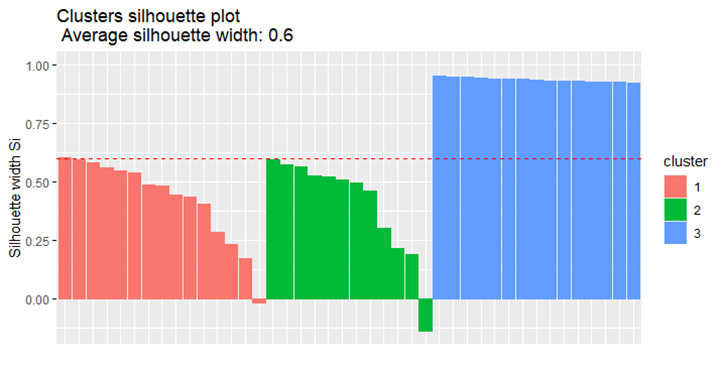
\includegraphics[width=\textwidth]{imgs/silhouette_umap_embeddings.png}
\caption*{(b) Gráfico de Silhouette}
\end{minipage}
\caption{Configuración inicial basada en embeddings, UMAP y clustering jerárquico con distancia coseno.}
\label{fig:umap_embeddings_inicial}
\end{figure}

La proyección muestra una separación visual más clara que las obtenidas con las matrices de palabras clave, mientras que el gráfico de Silhouette confirma un valor medio elevado, aunque con diferencias entre grupos. En particular, uno de los clusters aparece mucho más cohesionado que los demás, lo que indicaba que la configuración era prometedora, pero todavía requería una revisión más detallada antes de considerarse una solución definitiva.

Esta fase permitió comprobar que el cambio a embeddings era necesario desde el punto de vista metodológico, pero también que no resolvía por completo el problema de agrupamiento. La representación semántica reducía la dependencia de coincidencias literales entre palabras, aunque la calidad de los clusters seguía condicionada por la métrica utilizada, el método de agrupamiento, la reducción dimensional aplicada y el propio vocabulario de partida. Precisamente, la revisión de estas primeras agrupaciones permitió detectar que algunos términos no estaban contribuyendo a describir afinidades científicas, sino que introducían información contextual que solo aportaba ruido a la división. Esta observación motivó la depuración posterior del vocabulario antes de repetir las pruebas principales.

\subsection{Depuración del vocabulario y repetición del análisis}

La revisión de las primeras agrupaciones obtenidas con embeddings permitió detectar que el vocabulario de partida seguía influyendo de forma importante en los resultados. Aunque la representación semántica reducía la dependencia de coincidencias literales entre palabras clave, algunos términos no describían realmente ámbitos científicos, sino localizaciones geográficas u otros elementos contextuales asociados a determinadas revistas.

La presencia de este tipo de palabras podía afectar a la interpretación de los clusters, ya que introducía relaciones entre investigadores que no estaban necesariamente vinculadas a una afinidad temática real. Dos perfiles podían aparecer más próximos por compartir términos geográficos, por ejemplo, aunque esos términos no aportasen información relevante sobre las líneas de investigación. Por este motivo, se decidió revisar el vocabulario utilizado en la representación semántica y eliminar aquellas palabras que podían desplazar la agrupación hacia coincidencias poco informativas.

Esta depuración no supuso modificar el objetivo del análisis, sino ajustar la base textual para que respondiera mejor a dicho objetivo. La intención no era forzar una estructura de grupos determinada, sino reducir el ruido introducido por términos que no contribuían a describir áreas científicas. De esta forma, la comparación entre investigadores podía centrarse en palabras con mayor capacidad para representar afinidades temáticas.

Tras esta revisión manual, se generó una versión depurada del vocabulario y se repitieron las pruebas principales sobre la nueva base temática. No se repitieron todas las combinaciones exploradas en fases anteriores, sino aquellas que habían mostrado mayor interés metodológico o interpretativo. En particular, se volvieron a evaluar configuraciones basadas en embeddings, distintas medidas de proximidad, clustering jerárquico, métodos basados en densidad y reducciones de dimensionalidad como PCA y UMAP.

La Tabla~\ref{tab:pruebas_embeddings_sin_localizacion} resume algunas de las configuraciones más representativas obtenidas tras eliminar los términos de localización. Su objetivo no es sustituir la comparación final de modelos, sino mostrar cómo se comportaron las principales pruebas al trabajar con un vocabulario más ajustado al objetivo temático del análisis.

\begin{table}[H]
\centering
\small
\renewcommand{\arraystretch}{1.25}
\begin{tabular}{
>{\centering\arraybackslash}m{0.34\textwidth}
>{\centering\arraybackslash}m{0.18\textwidth}
m{0.38\textwidth}
}
\hline
\textbf{Configuración} & \textbf{Resultado} & \textbf{Observación principal} \\
\hline
Manhattan + Jerárquico & \(S=0.415\) & Resultado similar al vocabulario completo, manteniendo el problema de grupo dominante \\
\hline
Manhattan + PCA + Jerárquico & \(S=0.462\) & Mejora numérica respecto a la versión anterior, aunque persiste el problema de grupo dominante \\
\hline
Correlación + PCA + Jerárquico & \(S=0.552\) & Mejora clara tras la depuración, con una separación numérica más alta \\
\hline
Coseno + PCA + Jerárquico & \(S=0.551\) & Resultado elevado y comportamiento similar al de correlación \\
\hline
Coseno + DBSCAN & 2 clusters y 35.7\% de ruido & La reducción mediante PCA mejora el ruido, pero la estructura sigue siendo poco estable \\
\hline
Coseno + UMAP + Jerárquico & \(S=0.627\) & Mejor separación inicial, con estructura más clara tras la depuración \\
\hline
Manhattan + UMAP + Jerárquico & \(S=0.484\) & Resultado inferior al de coseno, aunque mantiene cierta separación \\
\hline
Euclídea + UMAP + Jerárquico & \(S=0.532\) & Resultado intermedio, con mejora respecto a algunas configuraciones directas \\
\hline
\end{tabular}
\caption{Resumen de pruebas realizadas tras la depuración del vocabulario.}
\label{tab:pruebas_embeddings_sin_localizacion}
\end{table}

Los resultados muestran que la depuración del vocabulario mejoró varias configuraciones relevantes, aunque no eliminó por completo los problemas observados en todos los modelos. Las pruebas basadas en distancia Manhattan siguieron presentando el problema de grupos dominantes, incluso cuando se aplicaba PCA, aunque sus valores de Silhouette aumentaron ligeramente. En cambio, las configuraciones con distancia de correlación o coseno tras PCA obtuvieron mejoras más claras respecto a las pruebas con el vocabulario completo, lo que indicaba una separación numérica más definida entre perfiles. También UMAP mantuvo un comportamiento favorable, con un valor de Silhouette superior al obtenido antes de la depuración. En general, la limpieza redujo parte del ruido del vocabulario y permitió obtener resultados más consistentes, pero no hizo que todas las configuraciones fueran igualmente válidas.

Los métodos basados en densidad, por su parte, continuaron mostrando limitaciones. En el caso de DBSCAN, incluso tras aplicar PCA y ajustar el parámetro \(\varepsilon\), seguía apareciendo una proporción importante de observaciones tratadas como ruido. Esto indicaba que los perfiles no formaban regiones densas suficientemente definidas para que este tipo de enfoque resultara adecuado como base principal del análisis.

La configuración con UMAP y clustering jerárquico volvió a destacar tras la depuración. En particular, la combinación con distancia coseno alcanzó un valor de Silhouette de 0.627, superior al obtenido en la fase previa con vocabulario completo. Este resultado reforzaba la idea de que la reducción no lineal podía ayudar a organizar los perfiles semánticos en una estructura más diferenciada, aunque todavía era necesario analizar la estabilidad y la interpretación temática de los grupos antes de seleccionar una configuración final.

Además de los valores de evaluación, también se revisó la composición de los grupos obtenidos tras la depuración, lo que permitió valorar si las palabras más representativas de cada cluster describían mejor ámbitos científicos y si los investigadores agrupados compartían perfiles temáticos coherentes. Por tanto, la evaluación de esta fase no se limitó a comparar métricas, sino que también incorporó una lectura cualitativa de la utilidad de las agrupaciones.

Con el vocabulario depurado, el análisis quedaba preparado para comparar con mayor detalle las configuraciones más relevantes. A partir de este punto, la atención podía centrarse en valorar qué combinaciones de medida de proximidad, reducción dimensional y método de clustering ofrecían agrupaciones más coherentes e interpretables. Esta comparación se desarrolla en el siguiente subapartado.

\subsection{Comparación final de configuraciones}

Una vez depurado el vocabulario y repetidas las pruebas principales, se realizó una comparación final entre las configuraciones más relevantes. El objetivo no era seleccionar automáticamente el modelo con mayor valor de Silhouette, sino evaluar conjuntamente dicho valor, la distribución de los investigadores entre grupos, la estabilidad de las particiones y la coherencia temática de los clusters obtenidos.

Para disponer de una medida cuantitativa común se utilizó el índice de Silhouette~\cite{rousseeuw}, que permite valorar hasta qué punto cada observación está mejor asignada a su propio grupo que a grupos alternativos. Para un investigador \(i\), este índice puede expresarse como:

\[
s(i) = \frac{b(i) - a(i)}{\max\{a(i), b(i)\}}
\]

donde \(a(i)\) representa la distancia media entre el investigador \(i\) y el resto de elementos de su mismo grupo, mientras que \(b(i)\) representa la menor distancia media entre \(i\) y los elementos de otro grupo. Valores próximos a 1 indican una asignación bien separada, valores cercanos a 0 reflejan grupos poco diferenciados y valores negativos sugieren que la observación podría estar más próxima a otro grupo.

No obstante, la interpretación del índice debía realizarse con cautela. En fases anteriores se había observado que algunas configuraciones podían alcanzar valores relativamente altos debido a la aparición de grupos dominantes, sin que ello implicara necesariamente una partición más útil desde el punto de vista temático. Por este motivo, la comparación final combinó la métrica cuantitativa con una revisión de la estructura de los grupos.

La Tabla~\ref{tab:comparacion_final_configuraciones} resume las configuraciones que resultaron más relevantes tras la depuración del vocabulario. Se incluyen tanto las alternativas con mejores valores numéricos como aquellas que ayudaron a descartar determinadas familias de métodos por problemas de interpretación o estabilidad.

\begin{table}[H]
\centering
\small
\renewcommand{\arraystretch}{1.25}
\begin{tabular}{
>{\centering\arraybackslash}m{0.34\textwidth}
>{\centering\arraybackslash}m{0.18\textwidth}
m{0.38\textwidth}
}
\hline
\textbf{Configuración} & \textbf{Resultado} & \textbf{Valoración final} \\
\hline
Coseno + UMAP + Jerárquico & \(S=0.627\) & Mejor separación numérica y visual, aunque con necesidad de revisar su estabilidad \\
\hline
Correlación + PCA + Jerárquico & \(S=0.552\) & Buen resultado numérico y útil como comparación frente a UMAP \\
\hline
Coseno + PCA + Jerárquico & \(S=0.551\) & Comportamiento muy similar al de correlación tras PCA \\
\hline
Euclídea + UMAP + Jerárquico & \(S=0.532\) & Resultado intermedio, con menor claridad que coseno sobre UMAP \\
\hline
Manhattan + UMAP + Jerárquico & \(S=0.484\) & Separación inferior respecto a coseno y euclídea sobre UMAP \\
\hline
Manhattan + PCA + Jerárquico & \(S=0.462\) & Mejora numérica, pero mantiene problemas de grupo dominante \\
\hline
Coseno + DBSCAN & 2 clusters y 35.7\% de ruido & No resultó adecuado como configuración final por la proporción de ruido \\
\hline
\end{tabular}
\caption{Comparación final de configuraciones tras la depuración del vocabulario.}
\label{tab:comparacion_final_configuraciones}
\end{table}

Los resultados muestran que las configuraciones basadas en reducción de dimensionalidad adquirieron mayor relevancia en la comparación final. En particular, la combinación de UMAP, distancia coseno y clustering jerárquico obtuvo el valor de Silhouette más alto y ofreció una separación visual más clara entre grupos, convirtiéndose en la configuración más prometedora desde el punto de vista cuantitativo y visual.

Las configuraciones basadas en PCA también ofrecieron resultados competitivos, especialmente al combinarse con distancias de correlación y coseno. Sin embargo, su interpretación debía compararse con la obtenida mediante UMAP, ya que una mejora numérica no siempre implicaba una organización más estable o más clara de los perfiles. En cambio, las configuraciones basadas en distancia Manhattan siguieron mostrando el problema de grupos dominantes, lo que reducía su utilidad como solución final pese a obtener valores aceptables de Silhouette.

En la configuración UMAP seleccionada, antes de aplicar la reducción no lineal se utilizó PCA para conservar el 90\% de la varianza, reduciendo previamente la dimensionalidad de los embeddings. Posteriormente, se aplicó UMAP con distancia coseno y clustering jerárquico con enlace \textit{average}.

La Figura~\ref{fig:umap_embeddings_depurado} muestra la configuración más destacada de la comparación final, basada en embeddings depurados, reducción mediante UMAP, distancia coseno y clustering jerárquico. Esta visualización permite observar la separación obtenida entre los grupos y complementa el valor medio de Silhouette mostrado en la Tabla~\ref{tab:comparacion_final_configuraciones}.

\begin{figure}[H]
\centering
\begin{minipage}{0.48\textwidth}
\centering
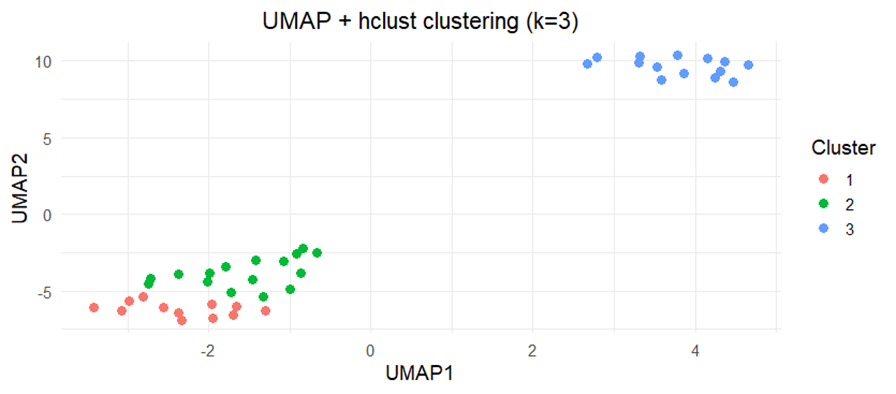
\includegraphics[width=\textwidth]{imgs/umap_coseno_jerarquico_depurado.png}
\caption*{(a) Proyección UMAP}
\end{minipage}
\hfill
\begin{minipage}{0.48\textwidth}
\centering
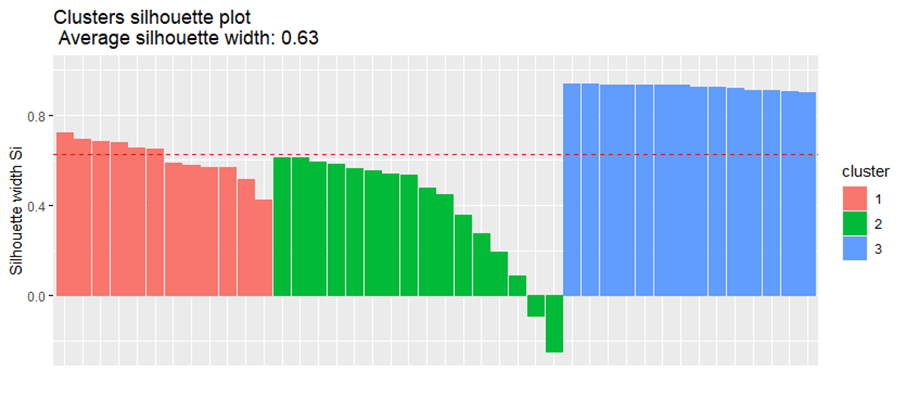
\includegraphics[width=\textwidth]{imgs/silhouette_umap_coseno_jerarquico_depurado.png}
\caption*{(b) Gráfico de Silhouette}
\end{minipage}
\caption{Configuración basada en embeddings depurados, UMAP y clustering jerárquico con distancia coseno.}
\label{fig:umap_embeddings_depurado}
\end{figure}

Como se puede observar, la buena puntuación global no se distribuye de forma completamente homogénea entre los grupos. Uno de los clusters aparece claramente separado y con valores de Silhouette altos, mientras que otros presentan observaciones más próximas al límite entre grupos. En consecuencia, esta configuración debía interpretarse junto con el análisis de estabilidad entre particiones y no únicamente a partir de su valor medio de Silhouette.

Los métodos basados en densidad no se consolidaron como alternativa final. Aunque DBSCAN permitía identificar observaciones que no encajaban claramente en ningún grupo, las pruebas realizadas seguían generando una proporción elevada de ruido y una estructura poco estable. Por este motivo, estos métodos resultaron útiles como contraste exploratorio, pero no como base principal para interpretar las afinidades temáticas entre investigadores.

La interpretación de los grupos no se limitó a las métricas y a las visualizaciones, sino que también incluyó una revisión de su composición temática. Para ello se analizaron las palabras clave más frecuentes en cada cluster, con el objetivo de comprobar si los grupos podían asociarse a ámbitos científicos diferenciados o si, por el contrario, respondían a términos demasiado generales. Esta revisión mostró que muchas de las palabras más representativas seguían siendo términos amplios, como \textit{research}, \textit{science}, \textit{academic}, \textit{journal} o \textit{education}, que describen el contexto académico de las revistas pero no permiten delimitar con precisión áreas temáticas concretas.

Además, la interpretación de las asociaciones semánticas se contrastó de forma cualitativa con el tutor del trabajo, conocedor del contexto investigador del IUMPA. Esta revisión permitió comprobar si algunas de las proximidades observadas resultaban razonables desde el punto de vista del dominio, aunque sin interpretar este contraste como una validación cerrada ni los grupos como una clasificación definitiva de los investigadores.

Esta revisión ayudó a matizar la interpretación de las agrupaciones obtenidas. Aunque los clusters podían reflejar ciertas proximidades entre perfiles, la presencia de palabras tan generales indicaba que no debían entenderse como áreas científicas cerradas ni como una clasificación estable de los investigadores. Por ello, también se revisó la distribución de investigadores entre grupos, ya que una partición con clusters muy descompensados o definidos por términos poco específicos podía resultar poco útil aunque alcanzara un buen valor numérico.

También se revisó el solapamiento entre particiones obtenidas con distintas configuraciones. Esta comparación permitía comprobar si modelos diferentes agrupaban a los mismos investigadores de forma similar o si las particiones cambiaban de manera importante al modificar la métrica, la reducción dimensional o el número de grupos. Para ello se compararon especialmente tres configuraciones: clustering jerárquico con distancia de correlación, clustering jerárquico con distancia coseno y clustering jerárquico con distancia coseno tras reducción mediante UMAP.

La comparación entre las configuraciones basadas en correlación y coseno mostró cierta correspondencia parcial entre algunos grupos, lo que indicaba la existencia de núcleos temáticos relativamente estables. Sin embargo, esta correspondencia no se mantenía de forma completa para todos los clusters, ya que varios grupos aparecían fragmentados o redistribuidos al cambiar la métrica de distancia.

La introducción de UMAP produjo una separación visual más clara, pero también modificó de forma notable la estructura de agrupamiento. Al comparar las particiones obtenidas con y sin UMAP, varios grupos diferenciados en los modelos jerárquicos originales aparecían concentrados en uno o dos clusters del modelo proyectado. Este comportamiento indicaba que la reducción no lineal influía de forma importante en la organización final de los grupos, por lo que sus resultados debían interpretarse junto con el análisis de solapamiento.

La Tabla~\ref{tab:solapamiento_configuraciones} resume las principales conclusiones obtenidas a partir de estas comparaciones entre particiones. Su objetivo no es recoger todas las matrices de solapamiento, sino sintetizar el comportamiento observado al enfrentar las configuraciones más relevantes.

\begin{table}[H]
\centering
\small
\renewcommand{\arraystretch}{1.25}
\begin{tabular}{
>{\centering\arraybackslash}m{0.34\textwidth}
m{0.56\textwidth}
}
\hline
\textbf{Comparación} & \textbf{Conclusión principal} \\
\hline
Correlación vs. Coseno & Correspondencia parcial entre algunos clusters, pero sin alineación global completa \\
\hline
Correlación vs. Coseno + UMAP & Ausencia de correspondencia directa entre particiones y concentración de coincidencias en clusters dominantes \\
\hline
Coseno vs. Coseno + UMAP & UMAP produce una separación visual más clara, pero altera de forma importante la organización previa de los grupos \\
\hline
\end{tabular}
\caption{Resumen cualitativo del solapamiento entre configuraciones seleccionadas.}
\label{tab:solapamiento_configuraciones}
\end{table}

La Figura~\ref{fig:solapamiento_umap_coseno} muestra el solapamiento entre la configuración jerárquica basada en distancia coseno y la misma configuración tras aplicar UMAP. Cada celda representa el número de investigadores compartidos entre clusters de ambas particiones.

\begin{figure}[H]
\centering
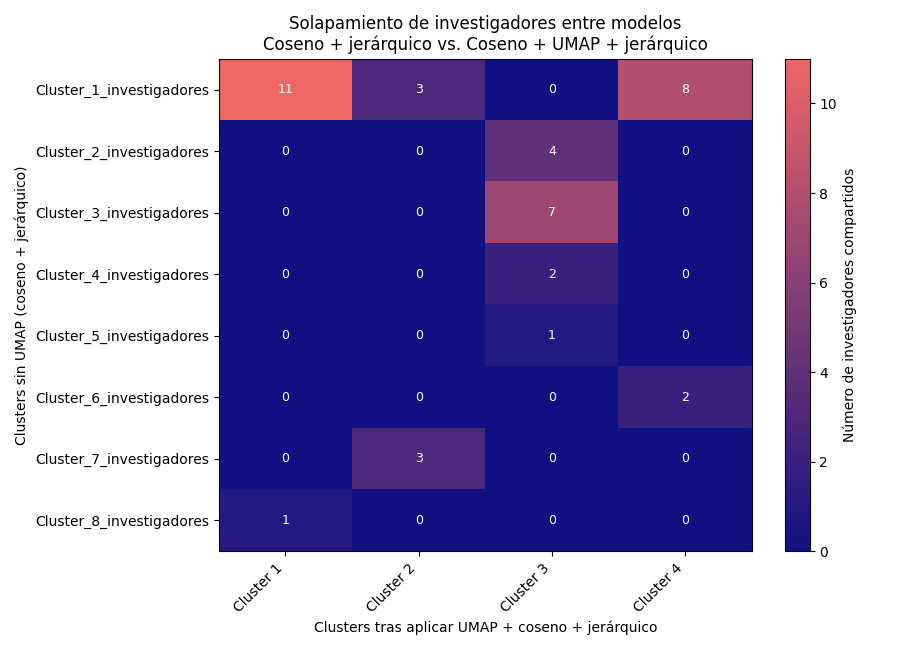
\includegraphics[width=0.78\textwidth]{imgs/solapamiento_investigadores_jerCos_vs_jerCosUMAP.png}
\caption{Solapamiento entre clustering jerárquico con distancia coseno y clustering jerárquico tras reducción mediante UMAP.}
\label{fig:solapamiento_umap_coseno}
\end{figure}

La comparación muestra que UMAP modifica de forma importante la organización de los grupos. Por ejemplo, el primer cluster del modelo sin UMAP se reparte entre varios clusters tras la proyección, con 11 investigadores en común con el cluster 1 de UMAP, 3 con el cluster 2 y 8 con el cluster 4. Al mismo tiempo, el cluster 3 de UMAP concentra investigadores procedentes de varios clusters del modelo original, incluyendo 4 del cluster 2, 7 del cluster 3, 2 del cluster 4 y 1 del cluster 5. Esto indica que la reducción mediante UMAP no solo cambia la visualización, sino también la estructura final del agrupamiento, por lo que sus resultados deben interpretarse con cautela.

Estos solapamientos mostraron que no existía una correspondencia estable y completa entre las particiones obtenidas por los distintos modelos. La estructura temática detectada era parcial y dependía de decisiones metodológicas como la métrica de distancia o la aplicación de reducción dimensional. Por tanto, aunque algunas configuraciones ofrecían resultados cuantitativamente buenos, no podía afirmarse la existencia de una arquitectura latente fuerte en los datos.

Esta conclusión también ayuda a interpretar el efecto de la depuración del vocabulario. La eliminación de términos de localización no creó por sí sola una estructura latente robusta, pero sí redujo una fuente de similitud no relacionada con el contenido científico. De este modo, las agrupaciones obtenidas tras la depuración resultaban más adecuadas para el objetivo temático del análisis, aunque seguían mostrando una estructura continua y parcialmente solapada.

Por tanto, la configuración basada en UMAP, distancia coseno y clustering jerárquico fue la más destacada desde los puntos de vista cuantitativo y visual, aunque las comparaciones entre modelos mostraron que la estructura temática no era completamente estable frente a cambios de métrica o de reducción dimensional. Por este motivo, sus resultados no deben interpretarse como una clasificación definitiva de los investigadores, sino como una aproximación exploratoria a posibles afinidades temáticas.

Aun así, los resultados obtenidos siguen siendo útiles para el objetivo exploratorio del trabajo. El clustering permite complementar la información relacional proporcionada por los grafos, ofreciendo una perspectiva adicional sobre posibles proximidades temáticas entre investigadores. Su valor principal no reside en definir una clasificación verdadera del IUMPA, sino en proporcionar una herramienta analítica que ayude a identificar agrupamientos plausibles que puedan ser interpretados con apoyo del conocimiento experto.

\section{Valoración del análisis semántico}

El análisis semántico permitió ampliar la explotación de la base de datos más allá de las relaciones explícitas representadas en los grafos. Mientras que los grafos muestran conexiones derivadas de publicaciones, revistas o proyectos compartidos, el clustering trató de explorar posibles afinidades temáticas entre investigadores a partir de las revistas en las que habían publicado y de las palabras clave asociadas a ellas. De este modo, esta parte del trabajo aportó una perspectiva complementaria a la visualización relacional desarrollada anteriormente.

El proceso seguido tuvo un carácter claramente experimental. Las primeras representaciones basadas en palabras clave explícitas resultaron útiles como punto de partida, pero mostraron las limitaciones de comparar perfiles únicamente mediante coincidencias literales. La ponderación del vocabulario permitió refinar esta representación, aunque no resolvió por completo el problema. El paso a embeddings semánticos supuso una mejora metodológica, ya que permitió comparar perfiles considerando la proximidad conceptual entre términos, pero también mostró que la calidad de las agrupaciones seguía dependiendo de la métrica utilizada, de la reducción dimensional y del vocabulario de partida.

Uno de los aspectos más relevantes del análisis fue la necesidad de revisar e interpretar los resultados de forma crítica. La depuración de términos de localización permitió reducir una fuente de similitud poco relacionada con el contenido científico, pero no generó por sí sola una estructura temática completamente estable. Del mismo modo, aunque algunas configuraciones alcanzaron valores de Silhouette relativamente altos, las comparaciones entre particiones mostraron que los grupos podían cambiar de forma apreciable al modificar la métrica o aplicar UMAP. Por ello, los clusters obtenidos deben entenderse como una aproximación exploratoria a posibles afinidades temáticas.

Esta interpretación también está condicionada por la naturaleza de los datos utilizados. Los perfiles se construyeron a partir de palabras clave asociadas a revistas, no a partir del contenido completo de los artículos ni de una validación experta exhaustiva de cada línea de investigación. Aunque algunas asociaciones se revisaron cualitativamente con el apoyo del tutor del trabajo, esta revisión debe entenderse como un apoyo interpretativo, no como una certificación formal de los grupos obtenidos.

A pesar de estas limitaciones, el análisis desarrollado aporta valor dentro del proyecto por varios motivos:

\begin{itemize}
    \item Permite justificar de forma razonada qué representaciones y métodos resultaron más adecuados para este tipo de datos.
    
    \item Muestra que la información temática disponible puede utilizarse para complementar la exploración visual de los grafos, ofreciendo una dimensión adicional basada en proximidad semántica.
    
    \item Deja abierta una base metodológica para futuras mejoras, entre ellas la incorporación de información textual más rica, una revisión más amplia del vocabulario con participación de otros especialistas, el uso de medidas de ponderación más elaboradas o la exploración de nuevas técnicas de representación y agrupamiento.
\end{itemize}

%%%%%%%%%%%%%%%%%%%%%%%%%%%%%%%%%%%%%%%%%%%%%%%%%%%%%%%%%%%%%%%%%%%%%%%%%%%%%%%
%                               BLOQUE III: cierre                            %
%%%%%%%%%%%%%%%%%%%%%%%%%%%%%%%%%%%%%%%%%%%%%%%%%%%%%%%%%%%%%%%%%%%%%%%%%%%%%%%

%%%%%%%%%%%
%Capítulo 7
%%%%%%%%%%%

\chapter{Conclusiones y trabajo futuro}

Al inicio del trabajo, la información sobre la actividad investigadora del IUMPA aparecía repartida entre distintas fuentes, con formatos y niveles de detalle diferentes. Esta situación hacía difícil obtener una visión conjunta del instituto y limitaba la posibilidad de analizar sus relaciones internas de forma clara. A partir de ese punto de partida, el proyecto ha consistido en transformar información dispersa en una base de datos estructurada, capaz de servir como soporte para la visualización y el análisis posterior.

Sobre esta base se ha desarrollado una aplicación interactiva que permite explorar visualmente parte de la información recopilada mediante grafos. Esta herramienta facilita una lectura más intuitiva de las relaciones existentes entre investigadores, revistas y proyectos, complementando la consulta directa de los ficheros tabulares. Además, el trabajo se ha ampliado con un análisis semántico destinado a estudiar afinidades temáticas entre investigadores a partir de las revistas en las que han publicado y de las palabras clave asociadas a dichas revistas.

Llegados a este punto, el capítulo final permite volver sobre el recorrido realizado y valorar qué se ha conseguido con respecto a los objetivos iniciales. Además de recoger las principales conclusiones del proyecto, se señalan las limitaciones que siguen presentes y las posibles líneas por las que el trabajo podría continuar. Finalmente, se deja constancia del material generado y se reflexiona sobre la relación entre el proyecto desarrollado y las competencias propias del Grado en Ciencia de Datos.

\section{Conclusiones generales}

Al cerrar el proyecto, la idea más importante que se extrae es que la información recopilada ha pasado de ser un conjunto de datos dispersos a convertirse en una base organizada para entender mejor la actividad investigadora del IUMPA. El trabajo no ha consistido únicamente en reunir registros, sino en darles una estructura, conectarlos entre sí y convertirlos en información útil para la visualización y el análisis. A partir de ello, ha sido posible estudiar el instituto desde los datos individuales de sus investigadores, pero también desde las relaciones y afinidades que aparecen entre ellos.

Uno de los resultados más relevantes del trabajo es la propia base de datos generada. A lo largo del proyecto, la información obtenida de las distintas fuentes fue tomando forma hasta convertirse en una estructura capaz de relacionar entre sí los principales elementos de la actividad investigadora del instituto. Esta organización permite pasar de una visión fragmentada, en la que cada dato aparece ligado a una fuente concreta, a una visión integrada en la que investigadores, publicaciones, revistas, proyectos y áreas pueden consultarse de forma conectada.

La dimensión alcanzada por la base de datos confirma que el trabajo no se ha quedado en una propuesta teórica. La información final reúne datos de 54 investigadores internos, 8 áreas de trabajo, 650 revistas, 4318 artículos y 281 proyectos únicos. Estos elementos, además, no se almacenan como registros independientes, sino que se relacionan entre sí para ofrecer una visión más completa de la actividad investigadora del IUMPA.

No obstante, una conclusión importante del proyecto es que el valor de la base de datos debe interpretarse siempre teniendo en cuenta las limitaciones de las fuentes utilizadas. La información procedía de recursos públicos, lo que conlleva distintos formatos y niveles de detalle. Por ello, la ausencia de determinados registros no debe entenderse como ausencia de actividad investigadora, sino como una consecuencia de la disponibilidad y calidad de la información accesible. Esta consideración ha estado presente durante todo el trabajo y ha condicionado tanto el diseño del modelo como la interpretación de los resultados.

A partir de la base de datos construida, la aplicación interactiva desarrollada permitió dar un paso más en la explotación de la información. La consulta directa de los ficheros resultantes podía ser útil desde un punto de vista técnico, pero no facilitaba una comprensión inmediata de las relaciones existentes entre los elementos del sistema. La representación mediante grafos permitió convertir esas relaciones en una visualización más accesible, en la que el usuario puede explorar conexiones entre investigadores, revistas y proyectos de forma más intuitiva.

La aplicación aporta valor porque transforma una base de datos estática en una herramienta de exploración. Los grafos desarrollados permiten observar relaciones derivadas de publicaciones compartidas y participación conjunta en proyectos, lo que facilita una lectura relacional de la actividad investigadora del instituto y permite consultar información que, en formato tabular, resultaría más difícil de interpretar de forma global. Su utilidad principal no está en sustituir a la base de datos, sino en hacerla más comprensible.

Otra aportación relevante del trabajo procede del análisis semántico de investigadores. Mientras que los grafos muestran relaciones explícitas, la agrupación semántica permitió explorar afinidades temáticas menos directas. Para ello, se partió de las revistas en las que habían publicado los investigadores y de las palabras clave asociadas a dichas revistas, construyendo representaciones temáticas que permitieran comparar perfiles investigadores desde una perspectiva distinta a la puramente relacional.

El proceso seguido en esta parte también muestra la importancia de no quedarse con la primera aproximación disponible. Las pruebas iniciales, basadas en coincidencias literales de palabras clave, no ofrecieron una separación suficientemente clara entre investigadores, por lo que se decidió revisar el enfoque y avanzar hacia representaciones semánticas mediante embeddings, capaces de incorporar relaciones conceptuales entre términos y de proporcionar una base más adecuada para el agrupamiento posterior.

Por ello, el interés de las agrupaciones obtenidas está en servir como apoyo para interpretar posibles afinidades temáticas entre investigadores, más que en fijar categorías definitivas entre ellos. Esta aportación complementa la información relacional proporcionada por los grafos, ya que permite observar cercanías entre perfiles que no siempre aparecen reflejadas mediante colaboraciones explícitas. Así, el análisis semántico añade una dimensión temática adicional que enriquece la comprensión de la estructura investigadora del IUMPA y deja abierta la posibilidad de seguir ampliando esta línea de trabajo.

Visto el recorrido completo, la principal aportación del trabajo está en haber unido tres niveles de análisis que se apoyan entre sí. Por ello, el resultado final no debe entenderse como una suma de partes independientes, sino como un marco coherente para consultar, visualizar y analizar la actividad investigadora del IUMPA desde varias perspectivas.

\section{Cumplimiento de los objetivos}

El objetivo principal del trabajo era organizar la información investigadora del IUMPA y desarrollar herramientas que permitieran analizarla de forma comprensible. Este objetivo se ha alcanzado mediante la construcción de una base de datos estructurada, el desarrollo de una aplicación interactiva basada en grafos y la incorporación de un análisis semántico orientado a estudiar afinidades temáticas entre investigadores. De este modo, la información recopilada no solo queda organizada, sino que puede explorarse visualmente y analizarse desde una perspectiva tanto relacional como temática.

A partir de este objetivo general, el trabajo planteaba una serie de objetivos específicos que han guiado las distintas fases del proyecto. Su grado de cumplimiento puede resumirse de la siguiente forma:

\begin{itemize}
    \item \textbf{Identificar las entidades y relaciones relevantes para describir la actividad investigadora del instituto.} Este objetivo se completó durante la fase de diseño conceptual, en la que se definieron los elementos principales del modelo y las conexiones necesarias para representar dicha actividad. A partir de este proceso se identificaron entidades como investigadores internos, revistas, áreas de trabajo y proyectos, junto con relaciones vinculadas a publicaciones, coautorías, participación en proyectos, colaboración en proyectos y pertenencia a áreas. Aunque el modelo inicial tuvo que modificarse durante el desarrollo, estos ajustes permitieron construir una estructura final más coherente con los datos realmente disponibles.

    \item \textbf{Recopilar información procedente de distintas fuentes públicas y transformarla en bases de datos organizadas y coherentes.} Este objetivo también se ha alcanzado, ya que el trabajo integró información institucional, bibliográfica, de proyectos y de caracterización temática procedente de varias fuentes accesibles públicamente. La información obtenida no se utilizó de forma directa, sino que fue organizada progresivamente en ficheros tabulares, de manera que pudiera servir como base para las tareas posteriores.

    \item \textbf{Resolver problemas de calidad de datos, duplicidad, formatos heterogéneos e información incompleta.} Este objetivo fue especialmente importante durante la construcción de la base de datos. La información recopilada presentaba inconsistencias propias de trabajar con fuentes públicas y heterogéneas, por lo que fue necesario combinar procedimientos automáticos con validaciones manuales para organizarla de forma coherente. Por tanto, el objetivo se considera cumplido dentro de las limitaciones derivadas de la calidad y disponibilidad de los datos.

    \item \textbf{Desarrollar una aplicación interactiva en R y Shiny que permita explorar visualmente la información mediante grafos.} Este objetivo se completó mediante la construcción de una herramienta que convierte la información estructurada en grafos interactivos. La aplicación permite explorar visualmente las relaciones recogidas en la base de datos e incorpora mecanismos de interacción y filtrado que facilitan la consulta sin necesidad de acceder directamente a los ficheros tabulares.

    \item \textbf{Analizar afinidades temáticas entre investigadores a partir de sus publicaciones y de las revistas en las que publican.} Este objetivo se alcanzó tomando como punto de partida las revistas asociadas a los artículos recopilados para cada investigador. A partir de estas revistas se construyó un vocabulario de palabras clave y se generaron representaciones temáticas de los perfiles investigadores. De este modo, fue posible estudiar similitudes entre investigadores desde una perspectiva diferente a la de las relaciones explícitas mostradas en los grafos.

    \item \textbf{Evaluar distintas estrategias de agrupación hasta obtener una representación temática suficientemente interpretable.} Este objetivo se ha cumplido con un carácter exploratorio. Durante el análisis se probaron distintas representaciones de los perfiles investigadores, pero también diferentes estrategias de agrupación, medidas de distancia y configuraciones de reducción de dimensionalidad. Las primeras pruebas con palabras clave explícitas, tanto en matrices binarias como ponderadas, no ofrecieron una separación suficientemente clara, por lo que se avanzó hacia representaciones semánticas mediante embeddings y clustering jerárquico. El resultado final no debe entenderse como una agrupación definitiva, sino como una representación temática suficientemente interpretable para apoyar el estudio de posibles afinidades entre investigadores.
\end{itemize}

En vista del recorrido realizado, los objetivos planteados al inicio de la memoria pueden considerarse alcanzados dentro del alcance definido para el trabajo. No obstante, el desarrollo también ha puesto de manifiesto las limitaciones derivadas de la disponibilidad y calidad de las fuentes, por lo que los resultados deben entenderse como una base útil y ampliable para seguir analizando la actividad investigadora del instituto.

\section{Líneas de trabajo futuro}

El trabajo desarrollado deja una base sobre la que pueden plantearse distintas ampliaciones. Estas líneas de mejora no deben entenderse como correcciones de un sistema incompleto, sino como posibles formas de continuar un proyecto que, por su propia naturaleza, puede crecer a medida que se incorporen nuevos datos, nuevas necesidades de consulta o nuevas técnicas de análisis.

Entre las principales líneas de trabajo futuro se pueden destacar las siguientes:

\begin{itemize}
    \item \textbf{Actualización, ampliación y mantenimiento de la base de datos.} La información recopilada procede de fuentes públicas y puede cambiar con el tiempo, ya que los investigadores publican nuevos artículos, participan en nuevos proyectos o modifican su información institucional. Por ello, una mejora natural sería definir un procedimiento de actualización periódica que permitiera incorporar nuevos registros sin reconstruir manualmente toda la base. Esta línea también podría incluir la incorporación de nuevas fuentes científicas no utilizadas en este trabajo y una mayor automatización en la regeneración de las estructuras principales, reduciendo la intervención manual en aquellas fases que puedan sistematizarse, sin perder la revisión supervisada de los casos ambiguos.

    \item \textbf{Consolidación de la información de proyectos.} En la versión actual, la información de proyectos queda asociada principalmente a los ficheros de participación de cada investigador. Como mejora futura, podría construirse un fichero específico de proyectos, con una fila por proyecto único y atributos normalizados, lo que facilitaría su actualización, reutilización y consulta independiente.

    \item \textbf{Mejora de la aplicación interactiva.} La aplicación podría ampliarse con nuevas funcionalidades de búsqueda, comparación, exportación de resultados o consulta resumida de determinados subconjuntos de información. También podrían incorporarse mejoras para navegar grafos densos o añadir métricas descriptivas de red que ayuden a interpretar mejor las relaciones visualizadas, manteniendo siempre el carácter exploratorio de la herramienta.

    \item \textbf{Exploración de nuevas técnicas de análisis semántico.} Futuras versiones podrían probar otras formas de representación y agrupamiento, como mapas autoorganizados (\textit{Self-Organizing Maps}, SOM) o nuevos modelos de embeddings más adaptados al dominio científico. También podrían incorporarse nuevas métricas de evaluación o criterios de comparación entre agrupaciones. Estas técnicas permitirían valorar si otros enfoques ofrecen representaciones temáticas más estables que las obtenidas en este trabajo.

    \item \textbf{Ampliación de la validación experta.} Aunque durante el trabajo se realizó una revisión cualitativa de algunas asociaciones semánticas con el apoyo del tutor del trabajo, una posible ampliación futura sería llevar a cabo una validación más sistemática con varios investigadores del IUMPA. Esto permitiría contrastar con mayor detalle la interpretación de los grupos y valorar si las proximidades observadas se corresponden con líneas de investigación reconocibles dentro del instituto.
\end{itemize}

\section{Legado}

El trabajo realizado deja una base aprovechable para futuras consultas, revisiones y ampliaciones. Su valor no reside solo en los resultados obtenidos, sino en haber construido un conjunto de recursos organizados que pueden seguir utilizándose más allá del desarrollo inicial del proyecto.

En primer lugar, la base de datos construida es una de las piezas centrales que quedan tras la finalización del trabajo. Los ficheros generados reúnen la información principal del proyecto y conservan las relaciones necesarias para su consulta, visualización y posible ampliación posterior. Gracias a ello, la información recopilada no queda limitada a los análisis realizados en esta memoria, sino que puede actualizarse posteriormente si se incorporan datos más completos.

En segundo lugar, la aplicación interactiva desarrollada también forma parte del legado del proyecto, ya que permite consultar la base de datos desde una perspectiva visual. Más allá de los grafos concretos incluidos en esta versión, la herramienta muestra cómo transformar las estructuras tabulares en visualizaciones explorables, por lo que podría ampliarse en el futuro con nueva información.

La aplicación interactiva queda disponible como prototipo asociado al proyecto a través del siguiente \href{https://cu2y3u-jos0antonio-rodr0guez0moreno.shinyapps.io/iumpa-grafos/}{enlace}. Su acceso y reutilización quedan condicionados por la disponibilidad de los ficheros de datos utilizados y por las consideraciones de protección de datos descritas en esta memoria.

La versión desplegada para consulta utiliza una versión limitada de los datos, excluyendo información de contacto, como los correos electrónicos, al no ser necesaria para la exploración visual. De este modo, se reduce la exposición de datos personales no imprescindibles y se mantiene el carácter exploratorio de la herramienta.

El trabajo también deja como legado una línea metodológica para el análisis temático de los investigadores. El proceso seguido, desde la construcción del vocabulario de palabras clave hasta la evaluación de distintas estrategias de agrupación, proporciona una referencia para continuar explorando afinidades temáticas a partir de la información disponible. Aunque los resultados obtenidos deben interpretarse con cautela, la metodología desarrollada permite identificar qué enfoques resultaron menos adecuados, qué limitaciones aparecieron y qué alternativas ofrecen una base más prometedora para futuras versiones.

No obstante, el acceso a estos materiales y su reutilización deben realizarse teniendo en cuenta la naturaleza de los datos tratados. Aunque la información procede de fuentes públicas, parte de ella está asociada a personas concretas, por lo que cualquier reutilización de la base debería tener en cuenta tanto las condiciones de uso de las fuentes consultadas como los criterios de protección de datos aplicables. Por este motivo, los materiales generados no deben entenderse necesariamente como un recurso abierto sin restricciones, sino como un conjunto de elementos que puede seguir evolucionando de forma controlada.

Así, los materiales generados ofrecen un punto de partida para seguir incorporando datos, nuevas formas de visualización y aproximaciones analíticas orientadas al estudio de la actividad investigadora del IUMPA.

\section{Relación del trabajo con el Grado en Ciencia de Datos}

Este trabajo se relaciona de forma directa con el Grado en Ciencia de Datos porque aborda un problema real en el que el valor no estaba en los datos por separado, sino en la capacidad de organizarlos, conectarlos e interpretarlos. A partir de información dispersa, el proyecto ha requerido construir una base coherente y utilizarla posteriormente para desarrollar herramientas de visualización y análisis.

En primer lugar, el trabajo ha permitido aplicar conocimientos relacionados con la preparación y tratamiento de datos. La información de partida procedía de fuentes públicas diversas, con formatos, niveles de completitud y criterios de identificación diferentes. Por ello, fue necesario organizar los datos, depurarlos, homogeneizarlos y construir estructuras coherentes que pudieran utilizarse posteriormente.

También se han aplicado competencias vinculadas al modelado y diseño de estructuras de datos. El proyecto exigió identificar entidades, relaciones y atributos relevantes para representar la actividad investigadora del IUMPA, así como adaptar el modelo inicial a las limitaciones reales de las fuentes disponibles. Esta parte conecta con la capacidad de transformar un problema del mundo real en una representación organizada y explotable, manteniendo la trazabilidad entre los datos originales y las estructuras finales.

La visualización de datos permitió dar una forma más accesible a la información construida. A través de la aplicación desarrollada en R y Shiny, las relaciones almacenadas en ficheros tabulares se transformaron en grafos interactivos que facilitaban su exploración, conectando el proyecto con la capacidad de presentar información compleja de manera comprensible.

Además, el análisis semántico de investigadores permitió aplicar conceptos propios de la recuperación de información (\textit{Information Retrieval}), el aprendizaje automático no supervisado y la representación vectorial de texto. Durante esta fase se construyeron perfiles temáticos y se compararon distintas formas de representar la información antes de evaluar varias estrategias de agrupación, lo que permitió comprobar que el resultado no dependía únicamente del algoritmo de clustering aplicado. También era necesario valorar cómo se construían los perfiles, qué información contenía el vocabulario, cómo se medía la similitud entre investigadores y hasta qué punto los grupos obtenidos resultaban interpretables.

El proyecto también ha requerido integrar conocimientos de programación y herramientas tecnológicas. Durante el desarrollo se emplearon lenguajes y entornos como R y Python, librerías específicas para gestionar los datos, así como fuentes externas que exigían adaptar los procedimientos a distintos formatos de información. Esta integración de herramientas refleja la necesidad de combinar conocimientos técnicos diversos para resolver problemas reales de datos.

Otro aspecto relacionado con el grado es la responsabilidad legal y ética en el uso de los datos. Aunque la información utilizada procedía de fuentes públicas, una parte estaba vinculada a investigadores concretos, por lo que el análisis se planteó con un alcance limitado y exploratorio, evitando utilizar los resultados para evaluar individualmente a los investigadores o establecer clasificaciones personales. Esta consideración permitió orientar el proyecto hacia un uso responsable de la información y coherente con la naturaleza de los datos tratados.

Desde el punto de vista de las competencias transversales, el trabajo ha requerido planificación, autonomía, toma de decisiones y capacidad de revisión crítica. Muchas decisiones no pudieron resolverse de forma automática, especialmente en la depuración de los datos recopilados, por lo que fue necesario combinar procedimientos técnicos con revisión manual y criterio interpretativo. Además, el carácter iterativo del proyecto obligó a revisar decisiones iniciales, descartar enfoques que no ofrecían resultados adecuados y justificar la evolución metodológica seguida.

En conclusión, este Trabajo Fin de Grado ha permitido aplicar una visión completa del trabajo con datos a un caso real. El desarrollo del proyecto no solo ha servido para poner en práctica conocimientos adquiridos durante la titulación, sino también para adaptarlos a las dificultades propias de trabajar con información pública, heterogénea y no preparada inicialmente para el análisis.

%%%%%%%%%%%%%%%%%%%%%%%%%%%%%%%%%%%%%%%%%%%%%%%%%%%%%%%%%%%%%%%%%%%%%%%%%%%%%%%
%                                BIBLIOGRAFIA                                 %
%%%%%%%%%%%%%%%%%%%%%%%%%%%%%%%%%%%%%%%%%%%%%%%%%%%%%%%%%%%%%%%%%%%%%%%%%%%%%%%

\begin{thebibliography}{99}

\bibitem{newmannetworks}
Newman, M. E. J.
\newblock \textit{Networks: An Introduction}.
\newblock Oxford University Press, 2010.

\bibitem{manning}
Manning, C. D., Raghavan, P. y Schütze, H.
\newblock \textit{Introduction to Information Retrieval}.
\newblock Cambridge University Press, 2008.

\bibitem{hastie}
Hastie, T., Tibshirani, R. y Friedman, J.
\newblock \textit{The Elements of Statistical Learning}.
\newblock Springer, 2009.

\bibitem{mikolov}
Mikolov, T., Chen, K., Corrado, G. y Dean, J.
\newblock Efficient Estimation of Word Representations in Vector Space.
\newblock \textit{arXiv preprint arXiv:1301.3781}, 2013.

\bibitem{RGPD2016}
Parlamento Europeo y Consejo de la Unión Europea.
\newblock \textit{Reglamento (UE) 2016/679 del Parlamento Europeo y del Consejo, de 27 de abril de 2016, relativo a la protección de las personas físicas en lo que respecta al tratamiento de datos personales y a la libre circulación de estos datos}.
\newblock Diario Oficial de la Unión Europea, 2016.

\bibitem{LOPDGDD2018}
Jefatura del Estado.
\newblock \textit{Ley Orgánica 3/2018, de 5 de diciembre, de Protección de Datos Personales y garantía de los derechos digitales}.
\newblock Boletín Oficial del Estado, núm. 294, 2018.

\bibitem{web_iumpa}
Instituto Universitario de Matemática Pura y Aplicada.
\newblock \textit{Web del Instituto Universitario de Matemática Pura y Aplicada}.
\newblock Disponible en: \url{https://iumpa.webs.upv.es/grupos-y-autores/}

\bibitem{google_scholar}
Google.
\newblock \textit{Google Scholar}.
\newblock Disponible en: \url{https://scholar.google.es/intl/es/scholar/about.html}

\bibitem{scopus}
Elsevier.
\newblock \textit{Scopus: Abstract and Citation Database}.
\newblock Disponible en: \url{https://www.elsevier.com/products/scopus}

\bibitem{orcid}
ORCID.
\newblock \textit{ORCID Public API Documentation}.
\newblock Disponible en: \url{https://info.orcid.org/documentation/api-tutorials/api-tutorial-read-data-on-a-record/}

\bibitem{panorama_upv}
Universitat Politècnica de València.
\newblock \textit{Panorama UPV: Portal de Producción y Actividad Científica}.
\newblock Disponible en: \url{https://www.upv.es/entidades/abdc/panorama-upv/}

\bibitem{doaj}
Directory of Open Access Journals.
\newblock \textit{Directory of Open Access Journals (DOAJ)}.
\newblock Disponible en: \url{https://doaj.org/}

\bibitem{scimago}
SCImago.
\newblock \textit{SCImago Journal \& Country Rank}.
\newblock Disponible en: \url{https://www.scimagojr.com/}

\bibitem{research_com}
Research.com.
\newblock \textit{Research.com}.
\newblock Disponible en: \url{https://research.com/}

\bibitem{r_scholar}
Yu, G., Keirstead, J. y Jefferis, G.
\newblock \textit{scholar: Analyse Citation Data from Google Scholar}.
\newblock R package.
\newblock Disponible en: \url{https://search.r-project.org/CRAN/refmans/scholar/html/scholar-package.html}

\bibitem{beugnon_scholar}
Beugnon, R.
\newblock \textit{Extract my scientific profile with R}.
\newblock Disponible en: \url{https://remybeugnon.netlify.app/post/extract-my-scientific-profile-with-r/}

\bibitem{shiny}
Chang, W., Cheng, J., Allaire, J., Sievert, C., Schloerke, B., Xie, Y., Allen, J.,
McPherson, J., Dipert, A. y Borges, B.
\newblock \textit{Shiny: Web Application Framework for R}.
\newblock R package.

\bibitem{echarts}
Apache Software Foundation.
\newblock \textit{Apache ECharts}.
\newblock Disponible en: \url{https://echarts.apache.org/}

\bibitem{salton}
Salton, G. y Buckley, C.
\newblock Term-weighting approaches in automatic text retrieval.
\newblock \textit{Information Processing \& Management}, 24(5), 513--523, 1988.

\bibitem{gaussian_function}
Mathwords.
\newblock \textit{Gaussian Function}.
\newblock Disponible en: \url{https://www.mathwords.com/g/gaussian_function.htm}.

\bibitem{sentencebert}
Reimers, N. y Gurevych, I.
\newblock Sentence-BERT: Sentence Embeddings using Siamese BERT-Networks.
\newblock \textit{Proceedings of the 2019 Conference on Empirical Methods in Natural Language Processing}, 2019.

\bibitem{minilm_multilingual}
Sentence Transformers.
\newblock \textit{paraphrase-multilingual-MiniLM-L12-v2}.
\newblock Disponible en: \url{https://huggingface.co/sentence-transformers/paraphrase-multilingual-MiniLM-L12-v2}.

\bibitem{umap}
McInnes, L., Healy, J. y Melville, J.
\newblock UMAP: Uniform Manifold Approximation and Projection for Dimension Reduction.
\newblock \textit{arXiv preprint arXiv:1802.03426}, 2018.

\bibitem{dbscan}
Ester, M., Kriegel, H.-P., Sander, J. y Xu, X.
\newblock A density-based algorithm for discovering clusters in large spatial databases with noise.
\newblock \textit{Proceedings of the Second International Conference on Knowledge Discovery and Data Mining}, 226--231, 1996.

\bibitem{hdbscan}
Campello, R. J. G. B., Moulavi, D. y Sander, J.
\newblock Density-based clustering based on hierarchical density estimates.
\newblock \textit{Advances in Knowledge Discovery and Data Mining}, 160--172, 2013.

\bibitem{jolliffe}
Jolliffe, I. T.
\newblock \textit{Principal Component Analysis}.
\newblock Springer, 2002.

\bibitem{rousseeuw}
Rousseeuw, P. J.
\newblock Silhouettes: A graphical aid to the interpretation and validation of cluster analysis.
\newblock \textit{Journal of Computational and Applied Mathematics}, 20, 53--65, 1987.

%%%%%%%%%%%%%%%%%%%%%%%%%%%%%%%%%%%%%%%%%%%%%%%%%%%%%%%%%%%%%%%%%%%%%%%%%%%%%%%
% MODEL D'ARTICLE                                                             %
%
%
%\bibitem{light}
%   Jennifer~S. Light.
%   \newblock When computers were women.
%   \newblock \textit{Technology and Culture}, 40:3:455--483, juliol, 1999.
%
%
% MODEL DE LLIBRE                                                             %
%
%
%\bibitem{ifrah}
%   Georges Ifrah.
%   \newblock \textit{Historia universal de las cifras}.
%   \newblock Espasa Calpe, S.A., Madrid, sisena edició, 2008.
%
%
% MODEL D'URL                                                                 %
%
%
%\bibitem{WAR}
%   Comunicat de premsa del Departament de la Guerra, 
%   emés el 16 de febrer de 1946. 
%   \newblock Consultat a 
%   \url{http://americanhistory.si.edu/comphist/pr1.pdf}.
%
%%%%%%%%%%%%%%%%%%%%%%%%%%%%%%%%%%%%%%%%%%%%%%%%%%%%%%%%%%%%%%%%%%%%%%%%%%%%%%%


\end{thebibliography}
\cleardoublepage


%%%%%%%%%%%%%%%%%%%%%%%%%%%%%%%%%%%%%%%%%%%%%%%%%%%%%%%%%%%%%%%%%%%%%%%%%%%%%%%
%                           APÈNDIXS  (Si n'hi ha!)                           %
%%%%%%%%%%%%%%%%%%%%%%%%%%%%%%%%%%%%%%%%%%%%%%%%%%%%%%%%%%%%%%%%%%%%%%%%%%%%%%%

\APPENDIX

%%%%%%%%%%%
%Anexo A
%%%%%%%%%%%

\chapter{Relación del trabajo con los Objetivos de Desarrollo Sostenible}

Este apéndice recoge la relación del Trabajo Fin de Grado con los Objetivos de Desarrollo Sostenible (ODS), de acuerdo con las directrices establecidas para la memoria. En este caso, la relación del proyecto con los ODS no se plantea desde una intervención social directa, sino desde la aportación que supone organizar información científica, facilitar su consulta y generar herramientas que puedan apoyar el análisis de la actividad investigadora.

El trabajo se vincula principalmente con objetivos relacionados con la investigación, la innovación, la educación superior y la colaboración científica. Esta relación debe interpretarse dentro del alcance real del proyecto, que se ha centrado en construir una base de datos, desarrollar una aplicación de visualización y plantear una metodología de análisis semántico.

A continuación se indican los objetivos con los que el trabajo guarda una relación más directa:

\begin{itemize}
    \item \textbf{ODS 9: Industria, innovación e infraestructura.}  
    Este es el ODS con el que el proyecto presenta una relación más clara. El trabajo contribuye a crear una infraestructura de información para organizar y explotar datos sobre la actividad investigadora del IUMPA. La base de datos construida permite reunir información que antes se encontraba dispersa, mientras que la aplicación interactiva facilita su consulta mediante grafos. De esta forma, el proyecto aporta una herramienta técnica que puede apoyar futuras tareas de análisis de la información científica.

    \item \textbf{ODS 4: Educación de calidad.}  
    El proyecto también se relaciona con este objetivo al desarrollarse en un contexto universitario y estar orientado a mejorar la comprensión de información académica e investigadora. La base de datos y las visualizaciones generadas pueden facilitar una lectura más clara de la actividad científica del instituto, sirviendo como apoyo para futuras consultas, trabajos académicos o ampliaciones relacionadas con la gestión del conocimiento dentro del ámbito universitario.

    \item \textbf{ODS 17: Alianzas para lograr los objetivos.}  
    Este objetivo aparece vinculado al trabajo por la importancia que tienen las relaciones de colaboración dentro del proyecto. Los grafos desarrollados permiten observar conexiones entre investigadores a partir de publicaciones compartidas y participación conjunta en proyectos. Además, el análisis semántico ofrece una vía complementaria para estudiar posibles proximidades temáticas entre perfiles investigadores. Aunque el proyecto no crea colaboraciones por sí mismo, sí proporciona una base que puede ayudar a identificar relaciones existentes y posibles afinidades útiles para futuras colaboraciones.
\end{itemize}

En resumen, la relación del trabajo con los ODS se centra principalmente en el apoyo a la investigación, la organización del conocimiento y la exploración de relaciones científicas. Su contribución no debe entenderse como un impacto directo y medido sobre estos objetivos, sino como una aportación técnica que puede facilitar futuras actividades de análisis dentro del contexto investigador del IUMPA.

%%%%%%%%%%%
%Anexo B
%%%%%%%%%%%

\chapter{Diccionario de datos y estructura de ficheros}
\label{ap:diccionario_datos}

Este apéndice documenta los principales ficheros generados durante la construcción de la base de datos, organizados en: entidades, relaciones y estructuras auxiliares para el análisis semántico.

\section{Ficheros de entidades}

Los ficheros de entidades recogen la información descriptiva de los principales elementos de la base de datos y sirvieron como referencia en distintas fases del proyecto.

\subsection{Investigadores internos}

El fichero \texttt{Investigadores\_internos.csv} contiene la información básica de los investigadores internos del IUMPA, entidad en torno a la cual se organizaban la mayoría de relaciones de la base de datos.

\begin{table}[H]
\centering
\small
\renewcommand{\arraystretch}{1.25}
\begin{tabularx}{\textwidth}{
>{\raggedright\arraybackslash}p{4cm}
>{\raggedright\arraybackslash}X
}
\toprule
\textbf{Atributo} & \textbf{Descripción} \\
\midrule
\texttt{Nombre} / \texttt{Nombre\_} & Nombre del investigador y variante normalizada utilizada como apoyo en la comparación con otras fuentes. \\
\midrule
\texttt{Identificador} & Código interno utilizado para identificar de forma única a cada investigador dentro de la base de datos. \\
\midrule
\texttt{Acronimo} & Variantes de firma o formas alternativas del nombre utilizadas para localizar y asociar registros procedentes de distintas fuentes. \\
\midrule
\texttt{Tipo de empleado} & Variable descriptiva que diferencia entre investigadores, becarios y becarios de investigación. \\
\midrule
\texttt{Girado} & Nombre en formato invertido, utilizado cuando alguna fuente presentaba el orden de nombre y apellidos de forma diferente. \\
\midrule
\texttt{Correos} & Dirección de contacto obtenida a partir de la información pública disponible. \\
\midrule
\texttt{Acortacion} & Forma abreviada del nombre empleada como identificador auxiliar en el tratamiento de los datos. \\
\bottomrule
\end{tabularx}
\caption{Atributos principales del fichero de investigadores internos.}
\label{tab:atributos_investigadores}
\end{table}

\begin{figure}[H]
\centering
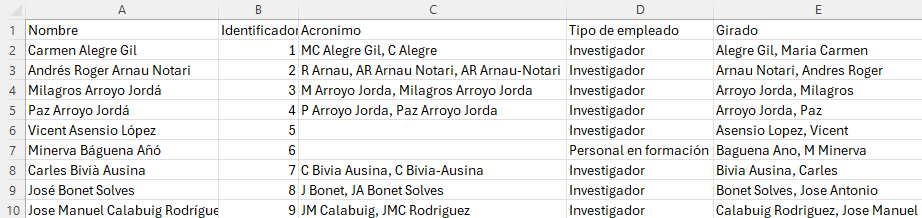
\includegraphics[width=\textwidth]{imgs/Investigadores_internos.png}
\caption{Ejemplo visual de la estructura parcial de \texttt{Investigadores\_internos.csv}.}
\label{fig:ejemplo_investigadores_internos}
\end{figure}

\subsection{Áreas de trabajo}

El fichero \texttt{Areas.csv} recoge el catálogo de áreas de trabajo identificadas a partir de la información pública del IUMPA. Estas áreas se conservaron como información auxiliar asociada a los investigadores y se utilizaron como criterio de filtrado en los grafos de la aplicación.

\begin{table}[H]
\centering
\small
\renewcommand{\arraystretch}{1.25}
\begin{tabularx}{\textwidth}{
>{\raggedright\arraybackslash}p{4cm}
>{\raggedright\arraybackslash}X
}
\toprule
\textbf{Atributo} & \textbf{Descripción} \\
\midrule
\texttt{Area} & Denominación del área de trabajo identificada. \\
\midrule
\texttt{Identificador} & Código interno utilizado para identificar cada área dentro de la base de datos. \\
\bottomrule
\end{tabularx}
\caption{Atributos principales del fichero de áreas de trabajo.}
\label{tab:atributos_areas}
\end{table}

\begin{figure}[H]
\centering
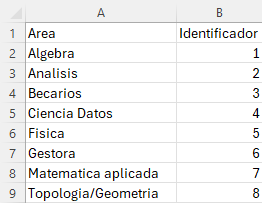
\includegraphics[width=0.3\textwidth]{imgs/Areas.png}
\caption{Ejemplo visual de la estructura del fichero \texttt{Areas.csv}.}
\label{fig:ejemplo_areas}
\end{figure}

\subsection{Revistas}

El fichero \texttt{Revistas.csv} contiene las revistas identificadas a partir de los artículos recopilados. Esta entidad permitió separar la información propia de las revistas de los registros de artículos y reutilizarla tanto en los grafos como en la fase de agrupación semántica.

\begin{table}[H]
\centering
\small
\renewcommand{\arraystretch}{1.25}
\begin{tabularx}{\textwidth}{
>{\raggedright\arraybackslash}p{4cm}
>{\raggedright\arraybackslash}X
}
\toprule
\textbf{Atributo} & \textbf{Descripción} \\
\midrule
\texttt{Revista} & Denominación de la revista o medio de publicación normalizado tras el proceso de depuración. \\
\midrule
\texttt{Identificador} & Código interno utilizado para identificar cada revista dentro de la base de datos. \\
\midrule
\texttt{Editorial} & Editorial asociada a la revista, cuando estaba disponible. \\
\bottomrule
\end{tabularx}
\caption{Atributos principales del fichero de revistas.}
\label{tab:atributos_revistas}
\end{table}

\begin{figure}[H]
\centering
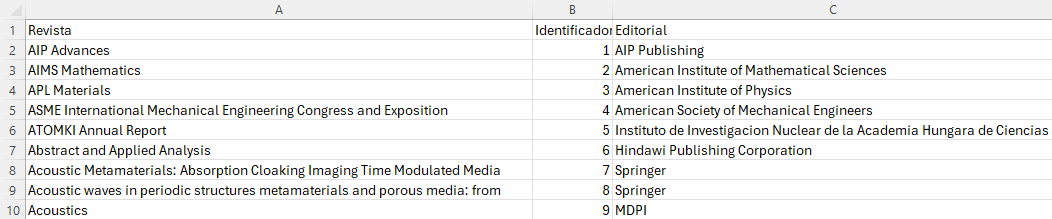
\includegraphics[width=0.85\textwidth]{imgs/Revistas.png}
\caption{Ejemplo visual de la estructura del fichero \texttt{Revistas.csv}.}
\label{fig:ejemplo_revistas}
\end{figure}

\section{Ficheros de relaciones}

Los ficheros de relaciones almacenan los vínculos entre las entidades de la base de datos. Estas estructuras fueron especialmente importantes para la aplicación interactiva, ya que algunas permitieron transformar la información tabular en nodos y enlaces, mientras que otras se utilizaron como información de filtrado.

\subsection{Relación entre investigadores y áreas}

El fichero \texttt{es\_parte\_de\_limpio\_listas.csv} recoge la relación entre investigadores internos y áreas de trabajo. Esta estructura permitió asociar cada investigador con las áreas identificadas en la fuente institucional y utilizar dicha asociación como criterio de filtrado en la aplicación.

\begin{table}[H]
\centering
\small
\renewcommand{\arraystretch}{1.25}
\begin{tabularx}{\textwidth}{
>{\raggedright\arraybackslash}p{4cm}
>{\raggedright\arraybackslash}X
}
\toprule
\textbf{Atributo} & \textbf{Descripción} \\
\midrule
\texttt{Nombre} & Nombre del investigador interno asociado a una o varias áreas de trabajo. \\
\midrule
\texttt{Areas} & Lista de áreas de trabajo vinculadas al investigador. \\
\bottomrule
\end{tabularx}
\caption{Atributos principales de la relación entre investigadores y áreas.}
\label{tab:atributos_es_parte_de}
\end{table}

\begin{figure}[H]
\centering
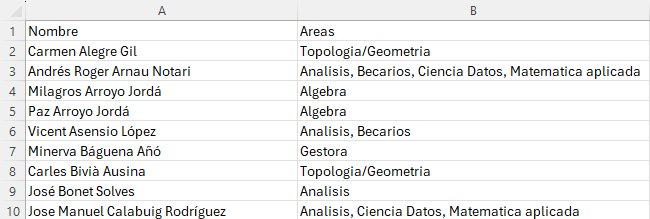
\includegraphics[width=0.85\textwidth]{imgs/es_parte_de.png}
\caption{Ejemplo visual de la estructura del fichero \texttt{es\_parte\_de\_limpio\_listas.csv}.}
\label{fig:ejemplo_es_parte_de}
\end{figure}

\subsection{Relación entre investigadores y revistas}

La relación \textit{ha\_publicado\_en} se almacenó mediante ficheros individuales por investigador. Por ello, el investigador no aparecía como una columna dentro del fichero, sino que quedaba identificado por el propio nombre del archivo. Estos ficheros recogen los artículos asociados a cada persona, la revista en la que fueron publicados y el año correspondiente.

\begin{table}[H]
\centering
\small
\renewcommand{\arraystretch}{1.25}
\begin{tabularx}{\textwidth}{
>{\raggedright\arraybackslash}p{4cm}
>{\raggedright\arraybackslash}X
}
\toprule
\textbf{Atributo} & \textbf{Descripción} \\
\midrule
\texttt{title} & Título del artículo recopilado para el investigador asociado al fichero. \\
\midrule
\texttt{journal} & Revista o medio de publicación asociado al artículo. \\
\midrule
\texttt{year} & Año de publicación del artículo. \\
\bottomrule
\end{tabularx}
\caption{Atributos principales de los ficheros de la relación entre investigadores y revistas.}
\label{tab:atributos_ha_publicado_en}
\end{table}

\begin{figure}[H]
\centering
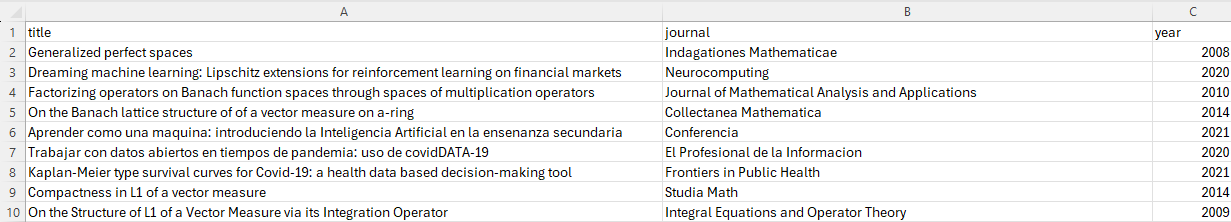
\includegraphics[width=\textwidth]{imgs/ha_publicado_en_JMCR.png}
\caption{Ejemplo visual de un fichero de la relación \textit{ha\_publicado\_en}.}
\label{fig:ejemplo_ha_publicado_en}
\end{figure}

\subsection{Relación de coautoría}

El fichero \texttt{ha\_publicado\_con.csv} recoge los coautores asociados a cada investigador a partir de los artículos recopilados. Esta estructura permitió construir relaciones de colaboración derivadas de artículos compartidos.

\begin{table}[H]
\centering
\small
\renewcommand{\arraystretch}{1.25}
\begin{tabularx}{\textwidth}{
>{\raggedright\arraybackslash}p{4cm}
>{\raggedright\arraybackslash}X
}
\toprule
\textbf{Atributo} & \textbf{Descripción} \\
\midrule
\texttt{nombre} & Nombre del investigador interno para el que se recoge la relación de coautoría. \\
\midrule
\texttt{otros\_inv} & Lista de autores con los que el investigador ha compartido artículos según la información recopilada. \\
\bottomrule
\end{tabularx}
\caption{Atributos principales del fichero de relación de coautoría.}
\label{tab:atributos_ha_publicado_con}
\end{table}

\begin{figure}[H]
\centering
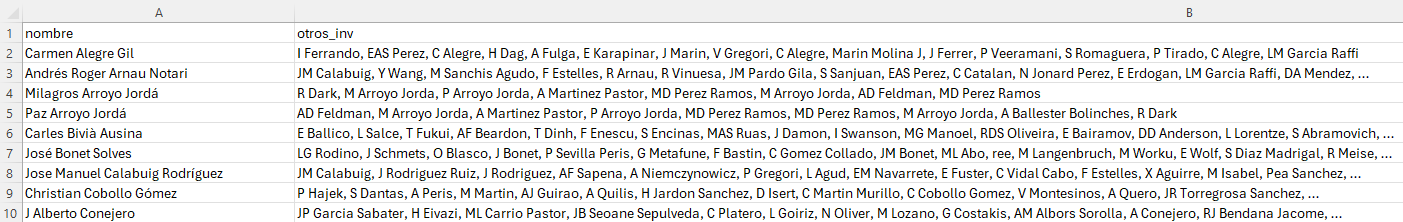
\includegraphics[width=\textwidth]{imgs/ha_publicado_con.png}
\caption{Ejemplo visual abreviado de la estructura de \texttt{ha\_publicado\_con.csv}.}
\label{fig:ejemplo_ha_publicado_con}
\end{figure}

\subsection{Relación entre investigadores y proyectos}

La relación \textit{ha\_participado\_en} se almacenó mediante ficheros individuales por investigador. Por ello, el investigador al que correspondía cada conjunto de proyectos quedaba identificado por el propio nombre del archivo. Estos ficheros recogen los proyectos asociados a cada persona, junto con información sobre sus participantes, fecha, identificador e indicación de investigador principal.

\begin{table}[H]
\centering
\small
\renewcommand{\arraystretch}{1.25}
\begin{tabularx}{\textwidth}{
>{\raggedright\arraybackslash}p{4.2cm}
>{\raggedright\arraybackslash}X
}
\toprule
\textbf{Atributo} & \textbf{Descripción} \\
\midrule
\texttt{TÍTULO} & Título o denominación del proyecto de investigación. \\
\midrule
\texttt{AUTORES} & Lista original de participantes del proyecto, conservando la información de rol cuando aparecía en la fuente. \\
\midrule
\texttt{FECHA} & Fecha asociada al proyecto en la información recopilada. \\
\midrule
\texttt{IDENTIFICADOR} & Código del proyecto dentro de la fuente original. \\
\midrule
\texttt{Es\_IP\_Principal} & Indicador lógico que señala si el investigador asociado al fichero actuaba como investigador principal en el proyecto. \\
\midrule
\texttt{INVESTIGADOR PRINCIPAL} & Nombre del investigador principal del proyecto, cuando estaba disponible. \\
\midrule
\texttt{AUTORES SIMPLIFICADO} & Lista de participantes normalizada, eliminando información sobre el rol para facilitar el tratamiento posterior. \\
\bottomrule
\end{tabularx}
\caption{Atributos principales de los ficheros de la relación entre investigadores y proyectos.}
\label{tab:atributos_ha_participado_en}
\end{table}

\begin{figure}[H]
\centering
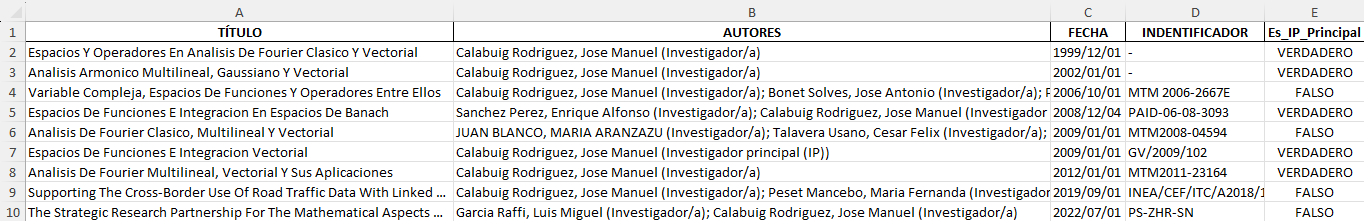
\includegraphics[width=\textwidth]{imgs/ha_participado_en_JMCR.png}
\caption{Ejemplo visual de la estructura parcial de \textit{ha\_participado\_en}.}
\label{fig:ejemplo_ha_participado_en}
\end{figure}

\subsection{Relación de colaboración en proyectos}

El fichero \texttt{ha\_participado\_con.csv} recoge las relaciones entre investigadores derivadas de la participación conjunta en proyectos. Esta estructura permitió representar colaboraciones basadas en proyectos, de forma complementaria a las colaboraciones obtenidas a partir de artículos compartidos.

\begin{table}[H]
\centering
\small
\renewcommand{\arraystretch}{1.25}
\begin{tabularx}{\textwidth}{
>{\raggedright\arraybackslash}p{4cm}
>{\raggedright\arraybackslash}X
}
\toprule
\textbf{Atributo} & \textbf{Descripción} \\
\midrule
\texttt{nombre} & Nombre del investigador interno para el que se recoge la relación de colaboración en proyectos. \\
\midrule
\texttt{otros\_inv} & Lista de participantes con los que el investigador ha coincidido en proyectos según la información recopilada. \\
\bottomrule
\end{tabularx}
\caption{Atributos principales del fichero de colaboración en proyectos.}
\label{tab:atributos_ha_participado_con}
\end{table}

\begin{figure}[H]
\centering
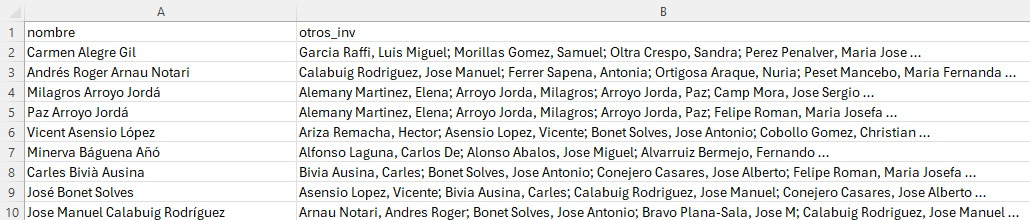
\includegraphics[width=\textwidth]{imgs/ha_participado_con.png}
\caption{Ejemplo visual abreviado de la estructura de \texttt{ha\_participado\_con.csv}.}
\label{fig:ejemplo_ha_participado_con}
\end{figure}

\section{Estructuras auxiliares para el análisis semántico}

Además de los ficheros utilizados para construir los grafos, se generaron estructuras auxiliares destinadas a preparar la fase de agrupación semántica. Estas estructuras permitieron trasladar la información de revistas y palabras clave al nivel de investigador, conservando la trazabilidad del origen de cada término.

\subsection{Matriz de revistas y palabras clave}

El fichero \texttt{One\_Hot\_Palabras\_Revistas\_filtrado.xlsx} representa la asociación entre revistas y palabras clave mediante una matriz de presencia y ausencia. Cada fila correspondía a una revista y las columnas indicaban la presencia de términos temáticos asociados a ella.

\begin{table}[H]
\centering
\small
\renewcommand{\arraystretch}{1.25}
\begin{tabularx}{\textwidth}{
>{\raggedright\arraybackslash}p{4cm}
>{\raggedright\arraybackslash}X
}
\toprule
\textbf{Elemento} & \textbf{Descripción} \\
\midrule
Filas & Cada fila representa una revista incluida en la matriz. \\
\midrule
Columnas & Cada columna, salvo la primera que representa a las revistas, representa una palabra clave temática. \\
\midrule
Valores binarios & Indican la asociación entre revista y palabra clave: 1 representa presencia de la palabra en la revista y 0 representa ausencia. \\
\bottomrule
\end{tabularx}
\caption{Estructura principal de la matriz de revistas y palabras clave.}
\label{tab:atributos_one_hot_revistas}
\end{table}

\begin{figure}[H]
\centering
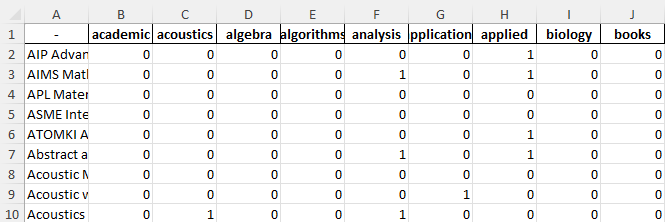
\includegraphics[width=0.75\textwidth]{imgs/one_hot_palabras_revistas_filtrado.png}
\caption{Ejemplo visual parcial de la matriz de revistas y palabras clave.}
\label{fig:ejemplo_one_hot_palabras_revistas}
\end{figure}

\subsection{Matriz de investigadores y palabras clave}

El fichero \texttt{Matriz\_Investigadores\_Keywords.xlsx} traslada la información temática al nivel de investigador. A partir de las revistas en las que había publicado cada persona, se asociaban a cada investigador los términos temáticos correspondientes.

\begin{table}[H]
\centering
\small
\renewcommand{\arraystretch}{1.25}
\begin{tabularx}{\textwidth}{
>{\raggedright\arraybackslash}p{4cm}
>{\raggedright\arraybackslash}X
}
\toprule
\textbf{Elemento} & \textbf{Descripción} \\
\midrule
Filas & Cada fila representa un investigador incluido en la matriz. \\
\midrule
Columnas & Cada columna, salvo la primera que representa al investigador, representa una palabra clave temática. \\
\midrule
Valores binarios & Indican la asociación entre investigador y palabra clave: 1 representa presencia de la palabra y 0 representa ausencia. \\
\bottomrule
\end{tabularx}
\caption{Estructura principal de la matriz de investigadores y palabras clave.}
\label{tab:atributos_matriz_investigadores_keywords}
\end{table}

\begin{figure}[H]
\centering
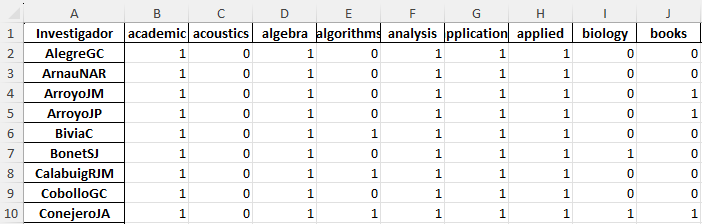
\includegraphics[width=0.8\textwidth]{imgs/matriz_investigadores_keywords.png}
\caption{Ejemplo visual parcial de la matriz de investigadores y palabras clave.}
\label{fig:ejemplo_matriz_investigadores_keywords}
\end{figure}

\subsection{Trazabilidad entre investigadores, revistas y palabras clave}

El fichero \texttt{Trazabilidad\_Keywords\_Revistas.xlsx} conserva la relación entre investigador, revista y palabra clave. Esta estructura permitió interpretar posteriormente el origen de los términos asociados a cada investigador.

\begin{table}[H]
\centering
\small
\renewcommand{\arraystretch}{1.25}
\begin{tabularx}{\textwidth}{
>{\raggedright\arraybackslash}p{4cm}
>{\raggedright\arraybackslash}X
}
\toprule
\textbf{Atributo} & \textbf{Descripción} \\
\midrule
\texttt{Investigador} & Investigador al que se asocia la información temática. \\
\midrule
\texttt{Revista} & Revista de la que proceden las palabras clave asociadas al investigador. \\
\midrule
\texttt{Keyword} & Término temático asociado a la revista y trasladado al perfil del investigador. \\
\bottomrule
\end{tabularx}
\caption{Atributos principales del fichero de trazabilidad temática.}
\label{tab:atributos_trazabilidad_keywords}
\end{table}

\begin{figure}[H]
\centering
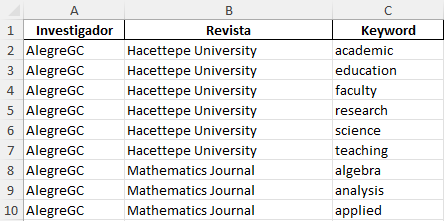
\includegraphics[width=0.5\textwidth]{imgs/trazabilidad_keywords_revistas.png}
\caption{Ejemplo visual parcial de trazabilidad entre investigadores, revistas y palabras clave.}
\label{fig:ejemplo_trazabilidad_keywords}
\end{figure}

\subsection{Listado auxiliar de revistas}

El fichero \texttt{Titulos\_revistas.json} recoge un listado auxiliar de revistas utilizado durante la preparación de la información temática. Este fichero sirvió como apoyo para organizar y consultar los títulos de revistas en la fase previa al análisis semántico.

\begin{table}[H]
\centering
\small
\renewcommand{\arraystretch}{1.25}
\begin{tabularx}{\textwidth}{
>{\raggedright\arraybackslash}p{4cm}
>{\raggedright\arraybackslash}X
}
\toprule
\textbf{Atributo} & \textbf{Descripción} \\
\midrule
Título de revista & Denominación de la revista incluida en el listado auxiliar. \\
\bottomrule
\end{tabularx}
\caption{Atributo principal del listado auxiliar de revistas.}
\label{tab:atributos_titulos_revistas}
\end{table}

%%%%%%%%%%%%%%%%%%%%%%%%%%%%%%%%%%%%%%%%%%%%%%%%%%%%%%%%%%%%%%%%%%%%%%%%%%%%%%%
%
% SI AÑADO MÁS APÉNDICES, MODIFICAR ÚLTIMO PÁRRAFO DE 1.4 Estructura de la memoria
%
%%%%%%%%%%%%%%%%%%%%%%%%%%%%%%%%%%%%%%%%%%%%%%%%%%%%%%%%%%%%%%%%%%%%%%%%%%%%%%%




%%%%%%%%%%%%%%%%%%%%%%%%%%%%%%%%%%%%%%%%%%%%%%%%%%%%%%%%%%%%%%%%%%%%%%%%%%%%%%%
%                              FI DEL DOCUMENT                                %
%%%%%%%%%%%%%%%%%%%%%%%%%%%%%%%%%%%%%%%%%%%%%%%%%%%%%%%%%%%%%%%%%%%%%%%%%%%%%%%


\end{document}